% Options for packages loaded elsewhere
% Options for packages loaded elsewhere
\PassOptionsToPackage{unicode}{hyperref}
\PassOptionsToPackage{hyphens}{url}
\PassOptionsToPackage{dvipsnames,svgnames,x11names}{xcolor}
%
\documentclass[
  letterpaper,
  DIV=11,
  numbers=noendperiod]{scrartcl}
\usepackage{xcolor}
\usepackage{amsmath,amssymb}
\setcounter{secnumdepth}{5}
\usepackage{iftex}
\ifPDFTeX
  \usepackage[T1]{fontenc}
  \usepackage[utf8]{inputenc}
  \usepackage{textcomp} % provide euro and other symbols
\else % if luatex or xetex
  \usepackage{unicode-math} % this also loads fontspec
  \defaultfontfeatures{Scale=MatchLowercase}
  \defaultfontfeatures[\rmfamily]{Ligatures=TeX,Scale=1}
\fi
\usepackage{lmodern}
\ifPDFTeX\else
  % xetex/luatex font selection
\fi
% Use upquote if available, for straight quotes in verbatim environments
\IfFileExists{upquote.sty}{\usepackage{upquote}}{}
\IfFileExists{microtype.sty}{% use microtype if available
  \usepackage[]{microtype}
  \UseMicrotypeSet[protrusion]{basicmath} % disable protrusion for tt fonts
}{}
\makeatletter
\@ifundefined{KOMAClassName}{% if non-KOMA class
  \IfFileExists{parskip.sty}{%
    \usepackage{parskip}
  }{% else
    \setlength{\parindent}{0pt}
    \setlength{\parskip}{6pt plus 2pt minus 1pt}}
}{% if KOMA class
  \KOMAoptions{parskip=half}}
\makeatother
% Make \paragraph and \subparagraph free-standing
\makeatletter
\ifx\paragraph\undefined\else
  \let\oldparagraph\paragraph
  \renewcommand{\paragraph}{
    \@ifstar
      \xxxParagraphStar
      \xxxParagraphNoStar
  }
  \newcommand{\xxxParagraphStar}[1]{\oldparagraph*{#1}\mbox{}}
  \newcommand{\xxxParagraphNoStar}[1]{\oldparagraph{#1}\mbox{}}
\fi
\ifx\subparagraph\undefined\else
  \let\oldsubparagraph\subparagraph
  \renewcommand{\subparagraph}{
    \@ifstar
      \xxxSubParagraphStar
      \xxxSubParagraphNoStar
  }
  \newcommand{\xxxSubParagraphStar}[1]{\oldsubparagraph*{#1}\mbox{}}
  \newcommand{\xxxSubParagraphNoStar}[1]{\oldsubparagraph{#1}\mbox{}}
\fi
\makeatother


\usepackage{longtable,booktabs,array}
\newcounter{none} % for unnumbered tables
\usepackage{calc} % for calculating minipage widths
% Correct order of tables after \paragraph or \subparagraph
\usepackage{etoolbox}
\makeatletter
\patchcmd\longtable{\par}{\if@noskipsec\mbox{}\fi\par}{}{}
\makeatother
% Allow footnotes in longtable head/foot
\IfFileExists{footnotehyper.sty}{\usepackage{footnotehyper}}{\usepackage{footnote}}
\makesavenoteenv{longtable}
\usepackage{graphicx}
\makeatletter
\newsavebox\pandoc@box
\newcommand*\pandocbounded[1]{% scales image to fit in text height/width
  \sbox\pandoc@box{#1}%
  \Gscale@div\@tempa{\textheight}{\dimexpr\ht\pandoc@box+\dp\pandoc@box\relax}%
  \Gscale@div\@tempb{\linewidth}{\wd\pandoc@box}%
  \ifdim\@tempb\p@<\@tempa\p@\let\@tempa\@tempb\fi% select the smaller of both
  \ifdim\@tempa\p@<\p@\scalebox{\@tempa}{\usebox\pandoc@box}%
  \else\usebox{\pandoc@box}%
  \fi%
}
% Set default figure placement to htbp
\def\fps@figure{htbp}
\makeatother

\ifLuaTeX
  \usepackage{luacolor}
  \usepackage[soul]{lua-ul}
\else
  \usepackage{soul}
\fi

% definitions for citeproc citations
\NewDocumentCommand\citeproctext{}{}
\NewDocumentCommand\citeproc{mm}{%
  \begingroup\def\citeproctext{#2}\cite{#1}\endgroup}
\makeatletter
 % allow citations to break across lines
 \let\@cite@ofmt\@firstofone
 % avoid brackets around text for \cite:
 \def\@biblabel#1{}
 \def\@cite#1#2{{#1\if@tempswa , #2\fi}}
\makeatother
\newlength{\cslhangindent}
\setlength{\cslhangindent}{1.5em}
\newlength{\csllabelwidth}
\setlength{\csllabelwidth}{3em}
\newenvironment{CSLReferences}[2] % #1 hanging-indent, #2 entry-spacing
 {\begin{list}{}{%
  \setlength{\itemindent}{0pt}
  \setlength{\leftmargin}{0pt}
  \setlength{\parsep}{0pt}
  % turn on hanging indent if param 1 is 1
  \ifodd #1
   \setlength{\leftmargin}{\cslhangindent}
   \setlength{\itemindent}{-1\cslhangindent}
  \fi
  % set entry spacing
  \setlength{\itemsep}{#2\baselineskip}}}
 {\end{list}}
\usepackage{calc}
\newcommand{\CSLBlock}[1]{\hfill\break\parbox[t]{\linewidth}{\strut\ignorespaces#1\strut}}
\newcommand{\CSLLeftMargin}[1]{\parbox[t]{\csllabelwidth}{\strut#1\strut}}
\newcommand{\CSLRightInline}[1]{\parbox[t]{\linewidth - \csllabelwidth}{\strut#1\strut}}
\newcommand{\CSLIndent}[1]{\hspace{\cslhangindent}#1}



\setlength{\emergencystretch}{3em} % prevent overfull lines

\providecommand{\tightlist}{%
  \setlength{\itemsep}{0pt}\setlength{\parskip}{0pt}}



 


\KOMAoption{captions}{tableheading}
\usepackage{fontspec}
\newfontfamily\ipaFont{Charis}
\newcommand{\ipa}[1]{{\ipaFont #1}}
\makeatletter
\renewcommand{\tableofcontents}{%
  \section*{Table of Contents}%
  \@starttoc{toc}%
}
\makeatother
\makeatletter
\@ifpackageloaded{caption}{}{\usepackage{caption}}
\AtBeginDocument{%
\ifdefined\contentsname
  \renewcommand*\contentsname{Table of contents}
\else
  \newcommand\contentsname{Table of contents}
\fi
\ifdefined\listfigurename
  \renewcommand*\listfigurename{List of Figures}
\else
  \newcommand\listfigurename{List of Figures}
\fi
\ifdefined\listtablename
  \renewcommand*\listtablename{List of Tables}
\else
  \newcommand\listtablename{List of Tables}
\fi
\ifdefined\figurename
  \renewcommand*\figurename{Figure}
\else
  \newcommand\figurename{Figure}
\fi
\ifdefined\tablename
  \renewcommand*\tablename{Table}
\else
  \newcommand\tablename{Table}
\fi
}
\@ifpackageloaded{float}{}{\usepackage{float}}
\floatstyle{ruled}
\@ifundefined{c@chapter}{\newfloat{codelisting}{h}{lop}}{\newfloat{codelisting}{h}{lop}[chapter]}
\floatname{codelisting}{Listing}
\newcommand*\listoflistings{\listof{codelisting}{List of Listings}}
\makeatother
\makeatletter
\makeatother
\makeatletter
\@ifpackageloaded{caption}{}{\usepackage{caption}}
\@ifpackageloaded{subcaption}{}{\usepackage{subcaption}}
\makeatother
\usepackage{bookmark}
\IfFileExists{xurl.sty}{\usepackage{xurl}}{} % add URL line breaks if available
\urlstyle{same}
% fallback for those not using the hyperref driver hyperxmp:
\makeatletter
\@ifundefined{xmpquote}{\newcommand{\xmpquote}[1]{#1}}{}
\makeatother
\hypersetup{
  colorlinks=true,
  linkcolor={blue},
  filecolor={Maroon},
  citecolor={Blue},
  urlcolor={Blue},
  pdfcreator={LaTeX via pandoc}}


\author{}
\date{}
\begin{document}


\begin{titlepage}
    \centering

    
\includegraphics[width=0.2\textwidth]{logo.jpg}\par
    \vspace{0.5cm}

    {\Large Universität zu Köln \par}
    {\large Faculty of Arts and Humanities, Department of Linguistics \par}
    \vspace{1cm}
    
    {\Large\itshape Master's Thesis \par}
    \vspace{0.7cm}

    {\LARGE\bfseries Subject realisation in L2 Spanish: \par}
    {\LARGE\bfseries An extended reproduction and replication of \par} 
    {\LARGE\bfseries Kocher (2025) with L1 German and L1 English corpus data \par}
    \vspace{1cm}
    
        \begin{center}
        {\normalsize \textit{A Thesis Submitted in Partial Fulfillment of the Requirements for the Degree}}\\[0.25cm]
        
        {\Large Master of Arts}\\[0.25cm]
        {\normalsize \textit{in the}}\\[0.25cm]
        {\Large Master Linguistik}
    \end{center}
    \vfill
    {\large Author: Tiziana Ilie\par}
    {\large Matriculation Number: 7421401\par}
    \vspace{0.7cm}
    {\large Supervisor: Dr. Elen Le Foll\par}
    \vspace{0.7cm}

    {\large 30 September 2026\par}

\end{titlepage}

\newpage{}

\pagenumbering{roman}

\tableofcontents

\newpage{}

\listoffigures

\newpage{}

\listoftables

\newpage{}

\pagenumbering{arabic}

\section{Introduction}\label{sec-introduction}

Spanish is a null subject language (NSL), allowing subjects to be
omitted when they can be recovered from the discourse. Learners whose
first language (L1) is a non-NSL, such as German or English, therefore
need to acquire not only the formal possibility of null subjects but
also the linguistic and discourse conditions governing the use of null
subjects, overt pronouns, and determiner phrases (DPs). Previous
research on subject realisation in L2 Spanish has largely relied on
experimentally elicited data and has often focused on the distinction
between null and overt subjects, while differences within overt
subjects, between pronouns and DPs, have received comparatively little
attention (see Section~\ref{sec-influential-factors}). Kocher
(\citeproc{ref-kocher_subject_2025}{2025}) addresses this gap by
applying MuPDARF modelling, an innovative statistical approach from
learner corpus research, to naturally occurring L2 data. Using written
short-film descriptions from the CEDEL2 corpus, Kocher investigates the
variables that influence subject realisation among L1 German learners of
Spanish. The study therefore provides a suitable basis for reproduction
and further extension.

The present thesis reproduces and extends Kocher's
(\citeproc{ref-kocher_subject_2025}{2025}) study using the same CEDEL2
data and statistical analysis following the MuPDARF procedure (see
\citeproc{ref-gries_theres_2020}{Gries et al., 2020};
\citeproc{ref-flach_mupdar_2022}{Gries, 2022}). In addition, the L1
German dataset is enlarged to assess the robustness of the original
findings. Two close replications further extend the analysis by
introducing two gender-related variables. namely the grammatical gender
of the subject referents (\textsc{SubjectGenus}) and the gender of the
L2 speakers (\textsc{SpeakerGender}) participating in the task. The
extended analysis is conducted both on the enlarged L1 German dataset
and on an L1 English dataset. Comparing these two non-NSL groups allows
for an investigation of both similarities and differences in L2 Spanish
subject realisation.

The study addresses three main research questions. First, it
investigates the reproducibility and robustness of the findings reported
by Kocher (\citeproc{ref-kocher_subject_2025}{2025}). Second, it
examines whether subject realisation differs between L2 Spanish learners
with L1 German and L1 English. Third, it investigates whether the
gender-related variables influence the target-likeness of subject
realisation and whether they interact with other variables. The thesis
is structured as follows. Chapter 2 presents the theoretical background,
including relevant variables and theoretical approaches to L2 subject
realisation in Spanish, English, and German, as well as the
\emph{Interface Hypothesis} and \emph{Feature-Reassembly Hypothesis},
which have emerged from previous research in this field. Chapter 3
describes the corpus, data, methodology, and replication design. Chapter
4 presents the results of the four analyses. Chapter 5 discusses the
findings and examines qualitative examples from the corpus. Chapters 6
and 7 address the limitations of the study and present the conclusion,
respectively.

\section{Theoretical background}\label{sec-Background}

This chapter provides the theoretical background for the present study
by first comparing the different systems of subject realisation in
Spanish, English, and German. It then reviews the main linguistic and
discourse-related variables that have been identified as influencing
subject realisation in these three languages. Building on this
cross-linguistic comparison, the second part of the chapter turns to the
acquisition of subject realisation in L2 Spanish. It introduces the two
theoretical approaches that are particularly relevant to the present
study and reviews previous research on the acquisition of subject
realisation in L2 Spanish. The chapter concludes by presenting the three
research questions that guide the present study.

\subsection{Comparing L1 systems of subject
realisation}\label{sec-SubjectRealisationEsp}

\subsubsection{Subject realisation in
Spanish}\label{subject-realisation-in-spanish}

According to Chomsky, languages can be classified as ``pro-drop'' or
``non-pro-drop languages'' (\citeproc{ref-chomsky1993}{1993}: 240).
While non-pro-drop languages, such as English and French, obligatorily
require overt subjects in the form of pronouns or determiner phrases
(DPs), pro-drop languages, such as Spanish, Greek, and Italian, do not
require subjects to be overtly expressed (see
\citeproc{ref-torres_cacoullos_variationist_2019}{Torres Cacoullos and
Travis, 2019}: 2). In the latter, the subject of a sentence may remain
implicit or have ``a phonologically empty form''
(\citeproc{ref-casteele_exploratory_2020}{Casteele and Palomares Ortiz,
2020}: 437), commonly referred to as pro, a null subject, or a covert
subject.

Spanish has a rich inflectional system in which verbs are inflected for
person, number, tense, and aspect (see \citeproc{ref-ayoun2003}{Ayoun,
2003}: 82). As subject information is encoded through verbal agreement
and almost all Spanish verb forms are distinct, an omitted referential
subject pronoun can generally be recovered grammatically from the verb
form. Consequently, Spanish provides three main options for the
realisation of referential subjects, as illustrated in example 1:

\begin{quote}
\begin{enumerate}
\def\labelenumi{(\arabic{enumi})}
\item
  a. \ul{\emph{Charles Chaplin}} \emph{está caminando por la calle.}\\
  `Charles Chaplin is walking down the street.'\\
  (example ID 2\_1, kocher\_native\_data\_annotation.csv)

  b. \ul{\emph{Él}} \emph{está caminando por la calle.}\\
  `He is walking down the street.'\\
  (own example)

  c. \ul{Ø} \emph{Está caminando por la calle.}\\
  `Ø is walking down the street.'\\
  (own example)
\end{enumerate}
\end{quote}

The subject can be realised as a DP, such as \emph{Charles Chaplin} in
1a, or as an overt pronoun, such as \emph{él} in 1b. Alternatively, it
can remain unexpressed, resulting in a covert or null subject, as in 1c.
In all three sentences, the subject refers to the same person. In
Spanish narratives, null subjects and DPs are generally the most
frequently used forms of subject realisation
(\citeproc{ref-comajoan2006}{Comajoan, 2006}: 74).

The same three options are available for embedded subjects, as
illustrated in Examples 2a-c (see also \citeproc{ref-ayoun2003}{Ayoun,
2003}: 85):

\begin{quote}
\begin{enumerate}
\def\labelenumi{(\arabic{enumi})}
\setcounter{enumi}{1}
\item
  a. \emph{Al principio {[}Charles Chaplin{]} \ul{Ø}}\textsubscript{i}
  \emph{cree que \ul{el niño}}\textsubscript{j} \emph{ha caído de un
  edificio.}\\
  `At first, {[}Charles Chaplin{]} \ul{\emph{Ø}}\textsubscript{i} thinks
  \ul{the boy}\textsubscript{j} has fallen from a building.'\\
  (own example)

  b. \emph{Al principio {[}Charles Chaplin{]} \ul{Ø}}\textsubscript{i}
  \emph{cree que \ul{él}}\textsubscript{j} \emph{ha caído de un
  edificio.}\\
  `At first, {[}Charles Chaplin{]} \ul{\emph{Ø}}\textsubscript{i} thinks
  \ul{he}\textsubscript{j} has fallen from a building.'\\
  (own example)

  c. \emph{Al principio {[}Charles Chaplin{]} \ul{Ø}}\textsubscript{i}
  \emph{cree que} \ul{\emph{Ø}}\textsubscript{j} \emph{ha caído de un
  edificio.}\\
  `At first, {[}Charles Chaplin{]} \ul{\emph{Ø}}\textsubscript{i} thinks
  \ul{\emph{Ø}}\textsubscript{j} has fallen from a building.'\\
  (example ID 12\_4-5, kocher\_native\_data\_annotation.csv)
\end{enumerate}
\end{quote}

Although Spanish allows null subjects, their use varies considerably
across regional varieties and discourse types. In particular, rates of
unexpressed third-person subjects differ substantially across varieties.
For instance, in sociolinguistic interview narratives from Mexico City,
null subjects occur in 73\% of third-person singular (3sg) constructions
(\emph{N} = 450) and 88\% of third-person plural (3pl) constructions
(\emph{N} = 176) (\citeproc{ref-lastramartin2015}{Lastra and Martín
Butragueño, 2015}: 10). In narratives produced by Peninsular Spanish
speakers, 68.5\% of singular and plural subjects are null (\emph{N} =
402) (\citeproc{ref-comajoan2006}{Comajoan, 2006}: 60). Similarly, in
conversational Colombian Spanish, null subjects occur in 68\% of 3sg
instances (\emph{N} = 1431) and 50\% of 3pl instances (\emph{N} = 1389)
(\citeproc{ref-torres_cacoullos_variationist_2019}{Torres Cacoullos and
Travis, 2019}: 40). Further evidence of regional variation comes from
Dominican Spanish, where a decline in null subject use and elevated
rates of overt subject pronouns suggest a shift away from the pro-drop
patterns observed in other varieties
(\citeproc{ref-toribio2000}{Toribio, 2000}: 339).

This variation is particularly relevant to the acquisition of L2
Spanish. On the one hand, variation in subject realisation may provide
learners with a degree of flexibility in their use of overt and covert
subjects without necessarily violating target-language patterns. On the
other hand, the optionality of null subjects may make it more difficult
for learners to develop a consistent, rule-based understanding of the
conditions governing the choice between different forms of subject
realisation. Thus, acquiring subject realisation in Spanish involves not
only learning that subjects can be omitted, but also learning how the
different subject forms are used across linguistic and discourse
contexts.

\subsubsection{Subject realisation in English and
German}\label{sec-SubjectRealisationGermanEnglish}

German and English are non-NSLs, meaning that their standard varieties
generally require referential subjects to be overtly expressed. While
Spanish is a pro-drop language, facilitated by its rich inflectional
system, English and German cannot generally rely on verbal morphology to
identify the subject (see \citeproc{ref-ayoun2003}{Ayoun, 2003}: 84).
This difference is particularly evident in English, where verb
morphology remains largely invariant across persons. Consequently,
English requires overt subjects to express and disambiguate person, as
illustrated by the forms \emph{I drink, you drink,} and \emph{he/she
drinks}. Referential subjects can be realised as proper names or noun
phrases, as in 3a, or as pronouns, as in 3b.

\begin{quote}
\begin{enumerate}
\def\labelenumi{(\arabic{enumi})}
\setcounter{enumi}{2}
\item
  a. \ul{\emph{Charles Chaplin}} is walking down the street\emph{.}\\
  (own example)

  b. \ul{\emph{He}} is walking down the street.\\
  (own example)

  c. ?\ul{Ø} is walking down the street.'\\
  (own example)
\end{enumerate}
\end{quote}

Nevertheless, subject omission does occur in English under restricted
circumstances (\citeproc{ref-ayoun2003}{Ayoun, 2003}: 138). Further,
Torres Cacoullos and Travis show that, as in Spanish, the frequency of
unexpressed subjects varies across discourse types. In spoken data from
the USA, rates of unexpressed third-person human subjects are five times
higher in narratives than in conversation
(\citeproc{ref-torres_cacoullos_variationist_2019}{Torres Cacoullos and
Travis, 2019}: 2). They further report that omitted subjects are
slightly more frequent in third-person singular contexts (5\%, \emph{N}
= 3500) than in third-person plural contexts (2\%, \emph{N} = 6600)
(\citeproc{ref-torres_cacoullos_variationist_2019}{Torres Cacoullos and
Travis, 2019}: 40).

Subject omission in English can occur when two verbs are linked by
coordination and conjunction, as in \emph{I wrote home to my family and
Ø said} (\citeproc{ref-torres_cacoullos_variationist_2019}{Torres
Cacoullos and Travis, 2019}: 8; see also \citeproc{ref-quesada2020}{T.
Quesada and Lozano, 2020}: 960), or in imperative constructions
(\citeproc{ref-lindstrom2017}{Lindstrom, 2017}: 11). However, these
constructions are not generally considered instances of true null
subjects (see \citeproc{ref-torres_cacoullos_variationist_2019}{Torres
Cacoullos and Travis, 2019}: 8) and can also occur in Spanish (see
\citeproc{ref-etxebarriazuluaga2022}{Etxebarria Zuluaga, 2022}: 93).
Lindstrom's research further shows that English pro-drop is subject to
strict distributional constraints, as ``unexpressed subjects do not
occur in subordinate or interrogative clauses, nor in the environment of
a contracted auxiliary'' (\citeproc{ref-lindstrom2017}{Lindstrom, 2017}:
58). Instead, null subjects predominantly occur in third-person matrix
clauses and, less frequently, in first-person contexts. Their use also
increases with the accessibility of the referent
(\citeproc{ref-lindstrom2017}{Lindstrom, 2017}: 151).

A further phenomenon referred to as ``diary-drop''
(\citeproc{ref-scott2013}{Scott, 2013}: 69) occurs predominantly in
written language and comprises two distinct categories. The first
involves non-referential or expletive subjects, as illustrated in
example 4. The second comprises first- and third-person declarative
sentences, as illustrated in Examples 5 and 6
(\citeproc{ref-scott2013}{Scott, 2013}: 69). In these cases, overt
pronouns can replace the null subjects without affecting the meaning or
acceptability of the clause (see \citeproc{ref-scott2013}{Scott, 2013}:
73).

\begin{quote}
\begin{enumerate}
\def\labelenumi{(\arabic{enumi})}
\setcounter{enumi}{3}
\item
  \ul{Ø\emph{/It}} \emph{seems rude not to reply}\\
  (\citeproc{ref-scott2013}{Scott, 2013}: 70)
\item
  ?\ul{Ø\emph{/I}} \emph{walked to Westminster Hall}\\
  (\citeproc{ref-scott2013}{Scott, 2013}: 69)
\item
  ?\ul{Ø\emph{/He}} \emph{probably wants you to reply to his message}~\\
  (\citeproc{ref-scott2013}{Scott, 2013}: 69)
\end{enumerate}
\end{quote}

\hfill\break
These instances of subject omission further illustrate that
constructions such as 3c are grammatically marked in English and that
their acceptability depends on contextual variables. Such variables
include the degree of formality of the register, constraints related to
spatial or typographic limitations in written language, and contexts in
which precise identification of the referent is not essential to the
communicative function of the utterance (\citeproc{ref-scott2013}{Scott,
2013}: 75). The overall frequency of subject omission also differs
markedly between English and Spanish. Whereas Torres Cacoullos and
Travis report unexpressed first- and third-person singular human
subjects in 60\% of their Spanish data, such subjects occur in only 3\%
of the English data
(\citeproc{ref-torres_cacoullos_variationist_2019}{Torres Cacoullos and
Travis, 2019}: 1).

Like English, German is a non-null subject language and generally
requires subjects to be overtly realised through proper names, noun
phrases, or pronouns, as illustrated in example 7.

\begin{quote}
\begin{enumerate}
\def\labelenumi{(\arabic{enumi})}
\setcounter{enumi}{6}
\item
  a. \ul{\emph{Charles Chaplin}} \emph{geht die Straße entlang.}\\
  `Charles Chaplin is walking down the street.'\\
  (own example)

  b. \ul{\emph{Er}} \emph{geht die Straße entlang.}\\
  `He is walking down the street.'\\
  (own example)

  c. ?\ul{\emph{Ø}} \emph{geht die Straße entlang.}\\
  `?Ø is walking down the street.'\\
  (own example)
\end{enumerate}
\end{quote}

As in English, however, German permits subject omission under restricted
conditions. Trutkowski distinguishes between ``out-of-the-blue drops'',
which occur with first- and second-person subjects and can be identified
morphologically, and third-person \emph{topic drop}, in which the
referent can only be identified through the presence of a discourse
antecedent (\citeproc{ref-trutkowski_topic_2016}{Trutkowski, 2016}: 10).
The latter type of subject omission predominantly concerns third-person
subjects in declarative sentences occupying the topic position and is
therefore also referred to as ``topic drop''
(\citeproc{ref-schmitz_null_2016}{Schmitz et al., 2016}: 104). In such
cases, the subject can be omitted when its referent is sufficiently
salient.

Nevertheless, pro-drop is only marginally used by native speakers of
German. For instance, Schmitz reports a rate of only 4\% (\emph{N} =
1,286) in child-directed speech
(\citeproc{ref-schmitz_null-subject_2012}{Schmitz et al., 2012}: 208),
as illustrated in example 8. Subject omission is also considered
ungrammatical in subordinate clauses, as in example 9, or when the
prefield is occupied by another element, such as a \emph{wh}-expression,
as in example 10.

\begin{quote}
\begin{enumerate}
\def\labelenumi{(\arabic{enumi})}
\setcounter{enumi}{7}
\item
  ?\ul{\emph{Ø/Er}} \emph{sollte das lesen}\\
  `?Ø/He should read it'\\
  (\citeproc{ref-schmitz_null-subject_2012}{Schmitz et al., 2012}: 212)
\item
  \emph{Ich denke dass} \ul{*Ø\emph{/er}} \emph{das lesen sollte}\\
  `I believe that *Ø/he should read it'\\
  (\citeproc{ref-schmitz_null-subject_2012}{Schmitz et al., 2012}: 212)
\item
  \emph{Was sollte} \ul{*Ø\emph{/er}} \emph{unbedingt lesen?}\\
  `What should *Ø/he absolutely read?'\\
  (\citeproc{ref-schmitz_null-subject_2012}{Schmitz et al., 2012}: 212)
\end{enumerate}
\end{quote}

Furthermore, subject omission in German predominantly occurs in
colloquial, spoken, or dialectal varieties. Schmitz describes these
contexts as ones in which ``realisation and omission are
discourse-pragmatically neutral; they may only reflect a different
speech style, omissions belonging to an informal register''
(\citeproc{ref-schmitz_null-subject_2012}{Schmitz et al., 2012}: 206).
Thus, in both languages, English and German, subject omission are
relatively seldom and function differently than in Spanish (see
\citeproc{ref-liceras_topic-drop_1999}{Liceras and Díaz, 1999}: 1). This
suggests that the informal use of null subjects in English and German is
unlikely to have a strong influence on the choice of subject form in the
L2 data examined in the present study. However, as Kocher
(\citeproc{ref-kocher_subject_2025}{2025}: 5) points out, such patterns
may be more relevant when the analysis is based on informal spoken
rather than written corpus data. Rather than focusing on subject
omission alone, previous research has identified a range of variables
that influence L1 speakers' choice between overt and null subjects. The
following section reviews these variables and compares their relevance
across Spanish, English, and German.

\subsection{Influential variables in subject
realisation}\label{sec-influential-factors}

\subsubsection{Information structure}\label{sec-InformationStructure}

Kocher's study primarily identifies several major discourse-pragmatic
variables that influence subject realisation, namely information
structure, referential (dis)continuity, and, closely related to the
latter, contrast, as well as grammatical person. Information structure
distinguishes between newly introduced subjects and subjects that have
already been established in the discourse. In Spanish, newly introduced
subjects tend to be realised overtly, either as pronouns or DPs, whereas
subjects that have already been introduced tend to be realised as null
subjects (see \citeproc{ref-kocher_subject_2025}{Kocher, 2025}: 5).

Following Brucart's \emph{Principio de lexicalización de los
pronominales}, new information in discourse must be realised
phonetically in Spanish (\citeproc{ref-brucart_elision_1987}{1987}:
219). For Spanish, this principle is empirically supported by Comajoan,
whose results show that DPs are generally used to introduce new
referents (\citeproc{ref-comajoan2006}{Comajoan, 2006}: 60), whereas
already introduced referents tend to be taken up as null subjects. This
pattern can also be observed in example 11 from Kocher's and my
extracted L1 Spanish dataset:

\begin{quote}
\begin{enumerate}
\def\labelenumi{(\arabic{enumi})}
\setcounter{enumi}{10}
\item
  a. \ul{\emph{El protagonista}} \emph{está en una zona abandonada y
  deprimida},\\
  `The protagonist is in a derelict and run-down area,'\\
  (example ID 17\_6, kocher\_native\_data\_annotation.csv)

  b. \ul{\emph{Ø}} \emph{encuentra una lata con unas colillas}\\
  `Ø finds a tin containing some cigarette ends'\\
  (example ID 17\_7, kocher\_native\_data\_annotation.csv)
\end{enumerate}
\end{quote}

Example 11 is taken from one of the texts written by a native speaker in
the L1 dataset. In 11a, the protagonist is newly introduced into the
discourse and is therefore expressed by the definite DP \emph{el
protagonista}. In 11b, the second clause of the same sentence, the
subject is given and co-referential with the subject of the first
clause. It is therefore realised as a null subject.

In addition to Brucart's \emph{Principio de lexicalización de los
pronominales} (\citeproc{ref-brucart_elision_1987}{1987}: 219), this
pattern can also be explained by Gundel et al.'s
(\citeproc{ref-gundel1993}{1993}: 275) \emph{Givenness Hierarchy}. The
hierarchy proposes that different referring expressions, such as
pronouns or determiners, signal different levels of cognitive status or
activation of a referent in the hearer's mind. According to the
hierarchy, when a referent is given and in focus, it is typically
referred to by a pronoun in non-NSLs, i.e.~by the neutral \emph{it} in
English and \emph{es} in German.

For Spanish, the \emph{Givenness Hierarchy} associates null subject use
(\emph{Ø}) with referents that are in focus. Pronouns such as \emph{él}
(or, less commonly, \emph{este, ese, aquel, este} + noun) are used for
activated referents. For familiar but neither activated nor focused
referents, a demonstrative such as \emph{ese/aquel} + noun is used (see
\citeproc{ref-gundel1993}{Gundel et al., 1993}: 284; see also
\citeproc{ref-etxebarriazuluaga2022}{Etxebarria Zuluaga, 2022}:
84).\footnote{Posio connects the role of null subjects not only to
  givennes but also to the \emph{Accessability Hierarchy} of Ariel
  (\citeproc{ref-ariel1994}{1994}: 30), stating that ``the use of
  subject pronouns is considered to indicate a lower level of
  accessibility or givenness of the referent than the use of null
  anaphora which in turn requires that the referent is `at the current
  center of attention'\,'' (\citeproc{ref-posio2013}{2013}: 779).}

For English and German, this relationship between information status and
pronoun interpretation is supported by Hemforth et al.
(\citeproc{ref-hemforth2010}{2010}) and Ellert
(\citeproc{ref-ellert2013}{2013}), who, among others, found that native
speakers of different languages exhibit distinct antecedent biases when
interpreting overt pronouns in ambiguous contexts. Their results show
that, in ambiguous sentences, personal pronouns are preferentially
interpreted as referring to ``the first-mentioned topical antecedent''
(\citeproc{ref-ellert2013}{Ellert, 2013}: 3), which is typically the
subject. This pattern can be observed in both NSLs and non-NSLs, as
illustrated in examples 12 and 13.

\begin{quote}
\begin{enumerate}
\def\labelenumi{(\arabic{enumi})}
\setcounter{enumi}{11}
\item
  a. \ul{\emph{Der Briefträger}\textsubscript{i}} \emph{hat \ul{den
  Straßenfeger}}\textsubscript{\ul{j}} \emph{getroffen}

  b. \emph{bevor \ul{er}}\textsubscript{i/j} \emph{nach Hause ging.}\\
  (\citeproc{ref-hemforth2010}{{Hemforth et al.}, 2010}: 2218)
\item
  a. \ul{\emph{The postman}\textsubscript{i}} \emph{met \ul{the
  streetsweeper}}\textsubscript{\ul{j}}

  b. \emph{before \ul{he}}\textsubscript{i/j} \emph{went home.}\\
  (\citeproc{ref-hemforth2010}{{Hemforth et al.}, 2010}: 2218)
\item
  a. \ul{\emph{Juan}}\textsubscript{i} \emph{vio a
  \ul{Carlos}}\textsubscript{\ul{j}}

  b. \emph{cuando \ul{Ø}}\textsubscript{i} \emph{caminaba en la playa.}

  c. \emph{cuando \ul{él}}\textsubscript{i/j} \emph{caminaba en la
  playa.}\\
  (\citeproc{ref-keating2011}{Keating et al., 2011} : 197)
\end{enumerate}
\end{quote}

In both English and German, the referent introduced first is generally
considered the antecedent of the pronoun in the subordinate clause,
rather than the referent introduced subsequently. Given the differences
in pronominal realisation, however, this pattern does not apply to
Spanish in quite the same way. For Italian, another NSL, the
\emph{Position of Antecedent Strategy} (PAS) proposes that null subjects
tend to refer to subject antecedents, whereas pronouns show a stronger
preference for non-subject antecedents (see
\citeproc{ref-carminati2002}{Carminati, 2002}). Nevertheless, Bruscato
and Baptista found that Spanish native speakers also tend to interpret
overt pronouns in subordinate clauses (SC) as referring to the
first-mentioned referent, that is, the subject of the matrix clause
(MC), and therefore pattern relatively similarly to English and German.
In Spanish, however, this pattern is considerably weaker and less
consistent than the strong preference for null subjects, which represent
the unmarked form in Spanish (\citeproc{ref-bruscato2022}{Bruscato and
Baptista, 2022}: 12).

A similar pattern was reported by Keating et al.
(\citeproc{ref-keating2011}{2011}) in their study of monolingual Spanish
speakers, heritage Spanish speakers (HSs), and L2 learners of Spanish.
They found that ``the HSs were more likely to interpret an overt pronoun
as co-referential with a subject antecedent than the monolingually
raised Spanish speakers and the L2 learners''
(\citeproc{ref-keating2011}{Keating et al., 2011}: 210). Another
variable closely related to information structure is referential
(dis)continuity. Whereas information structure concerns whether a
referent is newly introduced or already given, referential
(dis)continuity considers how a referent is subsequently maintained or
shifted in the discourse. The following section therefore turns to
referential (dis)continuity and its role in subject realisation.

\subsubsection{Referential
(dis)continuity}\label{sec-ReferentialContinuity}

Referential (dis)continuity, also referred to as \emph{topic shift} or
\emph{subject continuity} in previous studies, concerns whether a
subject in subsequent discourse refers to the same referent
(\emph{continuity}) or to a different one (\emph{discontinuity}).
Grimshaw and Samek-Lodovici argue that ``dropping a referential argument
proves to be possible only when the missing argument is co-referential
with the topic of the clause'' (\citeproc{ref-grimshaw1998}{Grimshaw and
Samek-Lodovici, 1998}: 196). Since a referent must have already been
introduced to become the discourse topic, continuous referents tend to
be realised as null subjects, whereas discontinuous referents are more
often expressed by overt subject forms in Spanish (see also
\citeproc{ref-lozano2023}{Lozano et al., 2023}: 3).

This relationship between referential continuity and the form of the
referring expression is also reflected in Givón's hierarchy of Topic
Continuity in Discourse (\citeproc{ref-givuxf3n1983}{1983}: 3). The
hierarchy places indefinite DPs at the lowest and zero anaphora at the
highest level of referential continuity, with definite DPs and pronouns
occupying intermediate positions. Thus, DPs are generally associated
with less continuous referents, whereas pronouns and, in Spanish, null
subjects are associated with greater referential continuity. More
generally, there is an ``inverse relation between the degree of
prominence\footnote{See the following definitions of pragmatic
  prominence by von Heusinger \& Schumacher:\\
  „Def.1: Prominence is a relational property that singles out one
  element from a set of elements of equal type and structure.\\
  Def.2: Prominence status shifts in time (as discourse unfolds).\\
  Def.3: Prominent elements are structural attractors, i.e.~they serve
  as anchors for the larger structures they are constituents of, and
  they may license more operations than their competitors.''
  (\citeproc{ref-vonheusingerschumacher2019}{{von Heusinger and
  Schumacher}, 2019}: 3).} of an entity and its referential continuity
in discourse'' (\citeproc{ref-vonheusingerschumacher2019}{{von Heusinger
and Schumacher}, 2019}: 4). Prominent referents tend to recur throughout
the discourse, whereas less prominent referents are mentioned less
frequently and are therefore more likely to be discontinuous.

This is the reason why the remention of a referent using an DP, as in
example 15a is infelicitous and why native speakers tend to use a null
subject to refer to the firstly introduced, most prominent referent.
When recurring to an activated but less prominent referent, like
\emph{Elsa}, they predominantly use a pronoun, as in 15b (see
\citeproc{ref-casteele_exploratory_2020}{Casteele and Palomares Ortiz,
2020}: 441).

\begin{quote}
\begin{enumerate}
\def\labelenumi{\arabic{enumi}.}
\setcounter{enumi}{14}
\item
  a. *\ul{\emph{Ana}}\textsubscript{i} \emph{ama a
  \ul{Elsa}}\textsubscript{j}\emph{, y \ul{Ana}}\textsubscript{i}
  \emph{lo sabe} (subject continuity)\\
  `\ul{Ana}\textsubscript{i} loves \ul{Elsa}\textsubscript{j} and
  \ul{Ana}\textsubscript{i} knows it'

  b. \ul{\emph{Ana}}\textsubscript{i} \emph{ama a
  \ul{Elsa}}\textsubscript{j}\emph{, y \ul{Ø}}\textsubscript{i} \emph{lo
  sabe} (subject continuity: Ø = \emph{Ana})\\
  `\ul{Ana}\textsubscript{i} loves \ul{Elsa}\textsubscript{j} and
  \ul{\emph{Ø}}\textsubscript{i} knows it'

  c. \ul{\emph{Ana}}\textsubscript{i} \emph{ama a
  \ul{Elsa}\textsubscript{j}, y \ul{ella}}\textsubscript{j} \emph{lo
  sabe} (subject discontinuity: ella = \emph{Elsa})\\
  `\ul{Ana}\textsubscript{i} loves \ul{Elsa}\textsubscript{j} and
  \ul{she}\textsubscript{i} knows it'\\
  (\citeproc{ref-casteele_exploratory_2020}{Casteele and Palomares
  Ortiz, 2020}: 441)
\end{enumerate}
\end{quote}

The preference for null subjects with continuous referents is supported
by several studies of Spanish. Previous research by Rothman and Iverson
(\citeproc{ref-rothman2007}{2007}), Rothman
(\citeproc{ref-rothman_pragmatic_2009}{2009}), Keating et al.
(\citeproc{ref-keating2011}{2011}) and Jegerski et al.
(\citeproc{ref-jegerski2011}{2011}) confirmed this referential subject
usage and state that in Spanish native speaker data between 73\% and
80\% of null subjects in Spanish native speaker data refer to continuous
subjects, whereas only 36\% to 53\% of overt subjects do so (see
overview \citeproc{ref-casteele_exploratory_2020}{Casteele and Palomares
Ortiz, 2020}: 444). Comajoan's comparison of Spanish and English data
from the same \emph{Pear Film} task further illustrates this
cross-linguistic difference. Spanish speakers predominantly used null
subjects (78.5\%) to maintain referential continuity, followed by DPs
(11\%) and pronouns (2\%). English speakers, by contrast, primarily used
pronouns (63.8\%) and DPs (15.7\%), although null subjects also occurred
in 20.5\% of cases (\citeproc{ref-comajoan2006}{Comajoan, 2006}: 69).
The latter finding can be related to the restricted contexts in which
English permits subject omission, including coordination and informal
contexts, but also topic continuity (\citeproc{ref-quesada2020}{T.
Quesada and Lozano, 2020}: 960).

Comajoan argues that the low frequency of overt pronouns in Spanish
reflects their discourse function of resolving referential ambiguity.
Since the referent can usually be recovered from the context, overt
pronouns are mainly used when additional cues are required to
distinguish between competing referents (see
\citeproc{ref-comajoan2006}{Comajoan, 2006}: 68). Example 16 illustrates
this pattern:

\begin{quote}
\begin{enumerate}
\def\labelenumi{\arabic{enumi}.}
\setcounter{enumi}{15}
\item
  a. \emph{y en esto que en el camino (ah en pues) en la otra dirección
  viene \ul{una chica}}\textsubscript{i}\\
  `and in all this on the road ah then in the other direction is \ul{a
  girl}\textsubscript{i} coming'

  b. \ul{\emph{él}}\textsubscript{j} \emph{se}\textsubscript{j}
  \ul{\emph{la}}\textsubscript{i} \emph{queda mirando\\
  '}\ul{he}\textsubscript{j} stands there looking at
  \ul{her}\textsubscript{i}'

  c. \emph{y \ul{la chica}}\textsubscript{i} \emph{pues (le da)
  le}\textsubscript{j} \emph{quita (al chico) al niño}\textsubscript{j}
  \emph{el sombrero que \ul{Ø}}\textsubscript{j} \emph{llevaba.\\
  '}and \ul{the girl}\textsubscript{i} then takes the hat
  \ul{Ø}\textsubscript{j} was wearing.'\\
  (\citeproc{ref-comajoan2006}{Comajoan, 2006}: 68)
\end{enumerate}
\end{quote}

In 16a the discourse topic is shifted from the boy to the girl. Although
the boy is temporarily discontinuous, he remains highly activated and
can therefore be referred to by a pronoun in 16b. The girl, likewise,
can be referred to by the object pronoun \emph{la}. In 16c, the DP
\emph{el sombrero} `the hat' is used to introduce a new referent and to
disambiguate the context. Similarly, Lozano and Quesada report that
overt Spanish pronouns show a ``flexible'' bias towards both subject and
non-subject antecedents, but are infrequent and are often replaced by
repeated DPs, which show a clearer preference for non-subject
antecedents (\citeproc{ref-lozano2023}{Lozano et al., 2023}: 1).

English and German show a similar distinction between continuous and
discontinuous referents, but differ from Spanish in their preferred
forms of realisation. In both non-NSLs, personal pronouns are the
default means of maintaining referential continuity, whereas DPs are
predominantly used to signal discontinuity
(\citeproc{ref-quesada2020}{T. Quesada and Lozano, 2020}: 971-972;
\citeproc{ref-bosch_demonstrative_2003}{Bosch et al., 2003}: 67). In
Quesada and Lozano's English data, pronouns were used in 52.7\%
(\emph{N} = 58) of cases of referential continuity, compared with 16.4\%
(\emph{N} = 18) DPs and 30.9\% (\emph{N} = 34) null subjects. For
referential discontinuity, however, DPs were clearly preferred (79.4\%,
\emph{N} = 76), while pronouns occurred in 19.6\% (\emph{N} = 19) and
null subjects in only 1\% of cases (\citeproc{ref-quesada2020}{T.
Quesada and Lozano, 2020}: 970). Example 17 illustrates the use of all
three forms:

\begin{quote}
\begin{enumerate}
\def\labelenumi{\arabic{enumi}.}
\setcounter{enumi}{16}
\item
  a. \emph{One day, \ul{a small boy}}\textsubscript{i} \emph{decided to
  catch \ul{a frog}}\textsubscript{j}

  b. \emph{and \ul{Ø}}\textsubscript{i} \emph{keep
  \ul{it}}\textsubscript{j} \emph{in a jar.}

  c. \ul{\emph{The frog}}\textsubscript{i} \emph{was not a fan of this
  living arrangement} {[}\ldots{]}.\\
  (\citeproc{ref-quesada2020}{T. Quesada and Lozano, 2020} : 972)
\end{enumerate}
\end{quote}

In 17a, both referents are introduced by DPs. The null subject in 17b
refers back to the boy in a coordinated clause, while the frog remains
activated and is referred to by the pronoun \emph{it}. In 17c, the topic
shifts to the frog, which is subsequently realised as a DP.

German also uses demonstratives alongside DPs and personal pronouns,
particularly to initiate a topic shift towards a less prominent but
activated referent (\citeproc{ref-schumacher2015}{Schumacher et al.,
2015}: 1; \citeproc{ref-gundel1993}{Gundel et al., 1993}: 278). German
distinguishes between the demonstrative pronouns \emph{dieser, diese,
dieses} and the shorter d-pronoun forms \emph{der, die, das}. The latter
can signal a topic shift towards a less prominent or non-topical
referent (\citeproc{ref-buchholz2024}{{Buchholz and von Heusinger},
2024}: 1; \citeproc{ref-schumacher2015}{Schumacher et al., 2015}: 2;
\citeproc{ref-bosch2007}{Bosch and Umbach, 2007} : 67;
\citeproc{ref-diessel1999}{Diessel, 1999}: 96;
\citeproc{ref-vonheusingerschumacher2019}{{von Heusinger and
Schumacher}, 2019}: 3), as illustrated in example 18:

\begin{quote}
\begin{enumerate}
\def\labelenumi{\arabic{enumi}.}
\setcounter{enumi}{17}
\item
  a. \ul{\emph{Der Anwalt}}\textsubscript{i} \emph{sprach mit \ul{einem
  Klienten}}\textsubscript{j}\\
  `The lawyer talked to a client.'

  b. \emph{Da \ul{er}}\textsubscript{i}\emph{/\ul{der}}\textsubscript{j}
  nicht viel Zeit hatte, vereinbarten sie ein weiteres Gespräch nächste
  Woche.\\
  `Since he/he\textsubscript{DEM} didn't have much time, they agreed to
  have another meeting next week.'\\
  (\citeproc{ref-diessel1999}{Diessel, 1999}: 96).
\end{enumerate}
\end{quote}

In 18b, the personal pronoun \emph{er} is predominantly interpreted as
referring back to the subject \emph{der Anwalt} `the lawyer' and thus
maintains the previous discourse topic. The demonstrative \emph{der}, by
contrast, refers to the non-topical DP \emph{einen Klienten} `a client'
and signals a topic shift (see \citeproc{ref-diessel1999}{Diessel,
1999}: 96).

This is further supported by Bosch et al., whose results show that
personal pronouns had nominative (subject) antecedents in 86.7\% of
cases, whereas demonstratives referred to non-nominative antecedents in
76.4\% of cases (\citeproc{ref-bosch_demonstrative_2003}{2003}: 67).
However, when also taking DPs into account, Ellert et al.~found that
personal pronouns were the preferred form for both first- and
second-mentioned referents, although they were less preferred for second
(68\%) than for first-mentioned referents (87\%) (see
\citeproc{ref-ellert2012}{Ellert et al., 2012}: 47). As German has a
relatively flexible word order, with subject position not being
restricted to SVO order, several studies have also examined whether OVS
constructions affect the choice of anaphoric expression. They found
that, in subject-initial sentences, the first-mentioned DP of the
preceding clause is the preferred antecedent for a personal pronoun
(\citeproc{ref-bosch2007}{Bosch and Umbach, 2007};
\citeproc{ref-ellert2013}{Ellert, 2013};
\citeproc{ref-schumacher2016}{Schumacher et al., 2016}; but
\citeproc{ref-wilson2009}{Wilson, 2009}).

\subsubsection{Further influential variables}\label{sec-ClauseType}

Kocher's data include some first-person singular (1PS) pronoun use,
which tends to be realised overtly more frequently than third-person
subjects (\citeproc{ref-kocher_subject_2025}{Kocher, 2025}: 7). As these
1PS cases are relatively rare in both the native and learner data, and
the task mainly required participants to describe the plot of a film
sequence, the present study focuses on third-person subjects. Several
other variables may influence subject realisation and are discussed
briefly in the following sections.

\paragraph{Contrast}\label{contrast}

Kocher excluded contrast from her analysis (see
\citeproc{ref-kocher_subject_2025}{2025}: 7); it is therefore considered
here only briefly as a variable related to information structure and
referential (dis)continuity. Given subjects tend to be realised as null
subjects when they are not contrasted, whereas they tend to be realised
as overt subjects when they are contrastive
(\citeproc{ref-mayol_contrastive_2010}{Mayol, 2010}: 1;
\citeproc{ref-rothman2007}{Rothman and Iverson, 2007}: 335;
\citeproc{ref-cameron1992}{Cameron, 1992}: 87, 95). Cameron
distinguishes three types of contrast: \emph{Contrast of
Negation/Antonymy}, \emph{Contrast of Scalar Opposition}, and
\emph{Contrast of Alternatives}, illustrated in examples 19-21:

\begin{quote}
Contrast of Negation/Antonymy

\begin{enumerate}
\def\labelenumi{\arabic{enumi}.}
\setcounter{enumi}{18}
\tightlist
\item
  \ul{\emph{Yo}}\textsubscript{i} \emph{no soy bonita pero
  \ul{ellas}}\textsubscript{j}/*Ø \emph{son bonitas.}\\
  `\ul{I}\textsubscript{i} no am pretty but
  \ul{they}\textsubscript{j}/\ul{*Ø} are pretty.'\\
  (\citeproc{ref-cameron1992}{Cameron, 1992}: 89)
\end{enumerate}

Contrast of Scalar Opposition

\begin{enumerate}
\def\labelenumi{\arabic{enumi}.}
\setcounter{enumi}{19}
\tightlist
\item
  \ul{\emph{Mi señora}}\textsubscript{i} \emph{habla bien ingles pero
  \ul{yo}}\textsubscript{j}\ul{\emph{/}*Ø} \emph{lo hablo muy
  quebrado}.\\
  `\ul{My wife}\textsubscript{i} speaks well English but
  \ul{I}\textsubscript{j}/\ul{*Ø} it speak very brokenly.'\\
  (\citeproc{ref-cameron1992}{Cameron, 1992}: 84)
\end{enumerate}

Contrast of Alternatives

\begin{enumerate}
\def\labelenumi{\arabic{enumi}.}
\setcounter{enumi}{20}
\tightlist
\item
  \ul{\emph{Él}}\textsubscript{i} \emph{tenia un toquecito de la monga
  ayer pero \ul{yo}}\textsubscript{j}\ul{\emph{/*Ø}} \emph{tengo la cosa
  verdadera hoy.}\\
  `\ul{He}\textsubscript{i} had a touch of the flu yesterday but
  \ul{I}\textsubscript{j}/*Ø have the real thing today.'\\
  (\citeproc{ref-cameron1992}{Cameron, 1992}: 95)
\end{enumerate}
\end{quote}

In all three examples, the second clause introduced by \emph{pero}
(`but') establishes a contrast between the subject of the first clause
and another activated referent. The contrastive subject is therefore
expressed by an overt pronoun rather than a null subject. Although the
referent in examples 20 and 21 can be identified from the first-person
singular verb forms \emph{hablo} (`I speak') and \emph{tengo} (`I
have'), the overt pronoun serves to emphasise the contrastive referent.
As Cameron notes, ``stress may also be involved in the obligatory use of
a subject pronoun here'' (\citeproc{ref-cameron1992}{1992}: 95). Thus,
null subjects are infelicitous in these contexts because they would fail
to express the intended contrast. In English and German, by contrast,
non-contrastive subjects can be realised as DPs or unstressed pronouns,
whereas contrastive subjects tend to be realised by stressed pronouns
(\citeproc{ref-kocher_subject_2025}{Kocher, 2025}: 7;
\citeproc{ref-quesada_l2_2015}{M. Quesada, 2015}: 28;
\citeproc{ref-garcuxeda-guerrero2026}{García-Guerrero and Lozano, 2026}:
372-375).

\paragraph{Clause Type}\label{clause-type}

Clause type is another variable that may affect subject realisation. In
Kocher's data, MCs predominantly contain null subjects (72\%, \emph{N} =
188), whereas pronouns predominantly occur in SC (73.5\%, \emph{N} = 61)
(\citeproc{ref-kocher_subject_2025}{Kocher, 2025}: 17). This pattern is
consistent with the findings of Liceras and Diaz
(\citeproc{ref-liceras_topic-drop_1999}{1999}: 32). Although null
subjects are somewhat less restricted in English than in German, they
are likewise predominantly found in declarative matrix clauses
(\citeproc{ref-torres_cacoullos_variationist_2019}{Torres Cacoullos and
Travis, 2019}: 1).

From a discourse perspective, rather than a language-specific one, this
distribution may be related to the discourse function of different
clause types. In narratives, the topic of one clause is often maintained
in the following clause, whereas SCs in non-coordinated structures,
which may serve functions such as elaboration, can involve a topic shift
(see \citeproc{ref-jegerski2011}{Jegerski et al., 2011}: 491). This is
also reflected in the findings of Torres Cacoullos and Travis, who
compared co-referential clauses linked by a coordinating conjunction
with clauses without such a conjunction in native English. They found
that coordinated clauses contained more null subjects than pronouns,
whereas co-referential contexts without coordination occurred less
frequently and showed a slightly higher proportion of pronominal
subjects (\citeproc{ref-torres_cacoullos_variationist_2019}{Torres
Cacoullos and Travis, 2019}: 8-9).

\paragraph{Subject Position}\label{subject-position}

Kocher explains that, in Spanish, the choice between the overt subject
forms DPs and pronouns can be influenced by the position of the subject
within a clause. Preverbal subjects are generally
information-structurally neutral, whereas postverbal subjects are
associated with focus. With unaccusative and presentative verbs,
however, this pattern is reversed, with the postverbal position being
information-structurally unmarked
(\citeproc{ref-kocher_subject_2025}{Kocher, 2025}: 15; see
\citeproc{ref-montrul2004}{Montrul, 2004}: 178). Thus, the preverbal
position in example 22 emphasises the subject, whereas the postverbal
position in example 23 represents the unmarked order (see
\citeproc{ref-alonso-ovalle2002}{Alonso-Ovalle et al., 2002}: 161).

\begin{quote}
\begin{enumerate}
\def\labelenumi{\arabic{enumi}.}
\setcounter{enumi}{21}
\tightlist
\item
  \emph{Juan vino}\\
  `John came'
\item
  \emph{Vino Juan}\\
  lit. `Came John'\\
  (\citeproc{ref-alonso-ovalle2002}{Alonso-Ovalle et al., 2002}: 161)
\end{enumerate}
\end{quote}

This distribution is also reflected in Kocher's data. Although preverbal
subjects are strongly preferred for both subject types, pronouns occur
almost exclusively preverbally, whereas postverbal DPs are more frequent
(\citeproc{ref-kocher_subject_2025}{Kocher, 2025}: 17). Only 5\%
(\emph{N} = 4) of pronouns occurred postverbally, compared with 22.5\%
(\emph{N} = 40) of DPs. These figures are lower than those reported by
Serrano and Aijón Oliva for Canarian Spanish (13.2\%, \emph{N} = 31) and
Peninsular Spanish (17.4\%, \emph{N} = 54)
(\citeproc{ref-serrano2010}{Serrano and Oliva, 2010}: 183), as well as
those reported for Spanish in New York City (1.5\%, \emph{N} = 929) by
Otheguy et al. (\citeproc{ref-otheguy2007}{Otheguy et al., 2007}: 771).

Subject position is also relevant to the \emph{Position of Antecedent
Hypothesis} (PAH), originally proposed by Carminati
(\citeproc{ref-carminati2002}{2002}) for Italian. The PAH predicts that
null subjects are more likely than pronouns to refer to prominent
antecedents, typically preverbal subjects, whereas pronouns are more
likely to refer to less prominent, typically postverbal antecedents.
Alonso-Ovalle et al. (\citeproc{ref-alonso-ovalle2002}{2002}), however,
show that this proposed ``division of labour''
(\citeproc{ref-alonso-ovalle2002}{2002}: 150) only partially applies to
Spanish. As preverbal constituents typically express the sentence topic,
a preverbal pronoun can also refer to a prominent subject antecedent,
thereby ``overriding the general preferences encoded in the PAH''
(\citeproc{ref-alonso-ovalle2002}{Alonso-Ovalle et al., 2002}). They
therefore argue that the apparent effects of the PAH may result from the
interaction between subject form and syntactic position, which itself
reflects the topic-focus structure of the sentence (see
\citeproc{ref-alonso-ovalle2002}{Alonso-Ovalle et al., 2002}: 150;
\citeproc{ref-quesada_l2_2015}{M. Quesada, 2015}: 128;
\citeproc{ref-wilson2009}{Wilson, 2009}: 31).

In English, preverbal subjects likewise tend to occupy the unmarked
topic position, whereas postverbal subjects are restricted to specific
constructions. These constructions include interrogatives, contexts
involving unaccusative verbs and constructions with focused or heavy
subjects that tend to be postverbal (\citeproc{ref-lozano2010}{Lozano
and Mendikoetxea, 2010}: 1). One example of such a construction is the
``\emph{there}-construction'', which occurs with verbs of ``existence
and appearance'' but not ``change of state''
(\citeproc{ref-lozano2010}{Lozano and Mendikoetxea, 2010}: 9): .

\begin{quote}
\begin{enumerate}
\def\labelenumi{\arabic{enumi}.}
\setcounter{enumi}{23}
\tightlist
\item
  \emph{There appeared \ul{a grotesque figure}}.\emph{\hfill\break
  (= A grotesque figure appeared)}
\item
  *\emph{There melted \ul{the butter}}.\\
  \emph{(= The butter melted)}\\
  (\citeproc{ref-lozano2010}{Lozano and Mendikoetxea, 2010}: 9)
\end{enumerate}
\end{quote}

Similarly to Spanish, postverbal subject position in English is closely
associated with information structure, particularly focus. Therefore,
subject position may indirectly affect the distribution of pronouns and
DPs by influencing the information-structural status of the referent.

German allows greater word-order flexibility than English but likewise
favours the preverbal domain as the unmarked position for topics (see
\citeproc{ref-kocher_subject_2025}{Kocher, 2025}: 17). Both SVO and OVS
orders are possible:

\begin{quote}
\begin{enumerate}
\def\labelenumi{\arabic{enumi}.}
\setcounter{enumi}{25}
\item
  a. \ul{\emph{Der Chefarzt}}\textsubscript{i} \emph{untersucht \ul{den
  Patienten}}\textsubscript{j}\emph{.} (SVO, preverbal)\\
  `\ul{The head doctor} is examining \ul{the patient}.'

  b. \ul{\emph{Den Patienten}}\textsubscript{j} \emph{untersucht \ul{der
  Chefarzt}}\textsubscript{i}\emph{.} (OVS, postverbal)\\
  = `\ul{The head} doctor is examining \ul{the patient}.'\\
  (\citeproc{ref-bosch2007}{Bosch and Umbach, 2007}: 3)
\end{enumerate}
\end{quote}

However, most studies on German do not directly examine the distribution
of DPs and pronouns across pre- and postverbal subject positions.
Instead, they investigate the interpretation of personal and
demonstrative pronouns in contexts containing potentially ambiguous
referents. Although this provides only indirect evidence for the role of
subject position in subject realisation, the findings are consistent
with Kocher's observation that German subjects are typically realised
preverbally (see \citeproc{ref-kocher_subject_2025}{2025}: 17). Bosch
and Umbach, for instance, found no significant effect of word order on
personal pronoun interpretation, as personal pronouns can refer to
subjects in both OVS and SVO contexts. Demonstratives, by contrast, were
significantly more likely to refer to objects than subjects. They
conclude that ``the relevant antecedent parameter would be rather
grammatical role than order of mention''
(\citeproc{ref-bosch2007}{2007}: 7; see also
\citeproc{ref-wilson2009}{Wilson, 2009}: 73). Thus, although subject
position may contribute to the interpretation of anaphoric expressions,
it does not determine their antecedent unambiguously. Consequently,
subject position may constrain the distribution of overt subject types
indirectly, but there is no direct evidence that preverbal or postverbal
position significantly determines the choice between a DP and a pronoun
(see \citeproc{ref-kocher_subject_2025}{Kocher, 2025}: 15).

\paragraph{Subject Genus and Speaker
Gender}\label{subject-genus-and-speaker-gender}

Da Cunha (2024) provides evidence that gender is relevant to the
distribution of human referents across syntactic functions and therefore
characterises it as a ``weak prominence feature''
(\citeproc{ref-dacunha2024}{2024}: iv), alongside other prominence
features such as \emph{animacy} and \emph{definiteness}. The results
indicate that this bias persists across different genres, discourse
statuses, subject positions, and semantic roles
(\citeproc{ref-dacunha2024}{2024}: iii). The strength of the bias also
differs according to the frequency of masculine and feminine nouns in
the respective languages: in the Spanish data, human subjects were
masculine in 79\% of cases, compared with 75\% in English
(\citeproc{ref-dacunha2024}{2024}: 154).

More specifically, Da Cunha finds that masculine human nouns are more
likely to occur as subjects than feminine nouns in both Spanish and
English. In Spanish, 78\% (\emph{N} = 2315) of masculine nouns occurred
as subjects, compared with 67\% (\emph{N} = 516) of feminine nouns. A
similar, although less pronounced, pattern was found in English, where
84\% (\emph{N} = 2209) of masculine nouns and 80\% (\emph{N} = 2209) of
feminine nouns occurred as subjects (\citeproc{ref-dacunha2024}{Da
Cunha, 2024}: 154).

The distribution of pronouns differs considerably between the two
languages. In Spanish, only 26\% (\emph{N} = 92) of masculine human
pronouns and 11\% (\emph{N} = 13) of feminine human pronouns occurred as
subjects, whereas in English, 87\% (\emph{N} = 3017) of masculine human
pronouns and 83\% (\emph{N} = 961) of feminine human pronouns occurred
as subjects (\citeproc{ref-dacunha2024}{Da Cunha, 2024}: 155). Thus, a
masculine bias in subject realisation is evident across both nouns and
pronouns (\citeproc{ref-dacunha2024}{Da Cunha, 2024}: 173).

For inanimate nouns in Spanish, by contrast, Da Cunha finds a relatively
balanced gender distribution, with approximately 52\% feminine and 48\%
masculine nouns. The proportion occurring as subjects is similarly
balanced, as 41\% of masculine and 39\% of feminine inanimate nouns
occurred in subject position (\citeproc{ref-dacunha2024}{2024}: 160).
The gender-related subject bias therefore appears to be specific to
human referents in the data. As Spanish lacks an inanimate subject
pronoun and pronominal subjects are generally infrequent and marked, no
comparable figures are available for inanimate pronouns
(\citeproc{ref-dacunha2024}{Da Cunha, 2024}: 160).

Da Cunha's model provides moderate evidence for an interaction between
gender and syntactic function, with masculine human referents more
frequently realised as subjects (\citeproc{ref-dacunha2024}{2024}: 175).
However, the study finds no evidence for an interaction between gender
and the choice of subject form, nor for a three-way interaction between
gender, syntactic function, and subject form
(\citeproc{ref-dacunha2024}{Da Cunha, 2024}: 175).

Furthermore, Da Cunha states that subject bias also correlates with the
social gender of the speakers, such that the more masculine the bias,
the higher the likelihood that the participant is male
(\citeproc{ref-dacunha2024}{2024}: 189). However, both women and men can
exhibit either a positive bias favouring male subjects or a negative
bias favouring female subjects (see \citeproc{ref-dacunha2024}{Da Cunha,
2024}: 189). The study further identifies an asymmetry in these biases,
as women are more likely to exhibit a neutral rather than a
female-favouring bias (see \citeproc{ref-dacunha2024}{Da Cunha, 2024}:
194).

\begin{longtable}[]{@{}
  >{\raggedright\arraybackslash}p{(\linewidth - 8\tabcolsep) * \real{0.1653}}
  >{\raggedright\arraybackslash}p{(\linewidth - 8\tabcolsep) * \real{0.1186}}
  >{\raggedright\arraybackslash}p{(\linewidth - 8\tabcolsep) * \real{0.1949}}
  >{\raggedright\arraybackslash}p{(\linewidth - 8\tabcolsep) * \real{0.1864}}
  >{\raggedright\arraybackslash}p{(\linewidth - 8\tabcolsep) * \real{0.3220}}@{}}
\caption{Own extended overview of Kocher's most relevant variables in
Spanish, German and English, focusing on the subject type predominantly
used (see \citeproc{ref-kocher_subject_2025}{Kocher, 2025}:
5).}\label{tbl-InfluentialFactors}\tabularnewline
\toprule\noalign{}
\begin{minipage}[b]{\linewidth}\raggedright
\end{minipage} & \begin{minipage}[b]{\linewidth}\raggedright
\end{minipage} & \begin{minipage}[b]{\linewidth}\raggedright
Spanish
\end{minipage} & \begin{minipage}[b]{\linewidth}\raggedright
English
\end{minipage} & \begin{minipage}[b]{\linewidth}\raggedright
German
\end{minipage} \\
\midrule\noalign{}
\endfirsthead
\toprule\noalign{}
\begin{minipage}[b]{\linewidth}\raggedright
\end{minipage} & \begin{minipage}[b]{\linewidth}\raggedright
\end{minipage} & \begin{minipage}[b]{\linewidth}\raggedright
Spanish
\end{minipage} & \begin{minipage}[b]{\linewidth}\raggedright
English
\end{minipage} & \begin{minipage}[b]{\linewidth}\raggedright
German
\end{minipage} \\
\midrule\noalign{}
\endhead
\bottomrule\noalign{}
\endlastfoot
Information structure & New &
\begin{minipage}[t]{\linewidth}\raggedright
DP,\\
(pronoun)\strut
\end{minipage} & DP & DP \\
\begin{minipage}[t]{\linewidth}\raggedright
\hfill\break
\strut
\end{minipage} & \begin{minipage}[t]{\linewidth}\raggedright
Given\\
\strut
\end{minipage} & \begin{minipage}[t]{\linewidth}\raggedright
Ø\\
\strut
\end{minipage} & \begin{minipage}[t]{\linewidth}\raggedright
pronoun\\
\strut
\end{minipage} & \begin{minipage}[t]{\linewidth}\raggedright
pronoun\\
\strut
\end{minipage} \\
Referential (dis)continuity & Discontinuous & DP, pronoun & DP,
(demonstrative) & DP, demonstrative \\
\begin{minipage}[t]{\linewidth}\raggedright
\hfill\break
\strut
\end{minipage} & \begin{minipage}[t]{\linewidth}\raggedright
Continuous\\
\strut
\end{minipage} & \begin{minipage}[t]{\linewidth}\raggedright
Ø\\
\strut
\end{minipage} & \begin{minipage}[t]{\linewidth}\raggedright
pronoun\\
\strut
\end{minipage} & \begin{minipage}[t]{\linewidth}\raggedright
pronoun\\
\strut
\end{minipage} \\
Clause Type & Matrix Clause (MC) & DPs, Ø & DP, pronoun & DP, pronoun \\
\begin{minipage}[t]{\linewidth}\raggedright
\hfill\break
\strut
\end{minipage} & \begin{minipage}[t]{\linewidth}\raggedright
Subordinated Clause (SC)\\
\strut
\end{minipage} & \begin{minipage}[t]{\linewidth}\raggedright
pronoun, Ø\\
\strut
\end{minipage} & \begin{minipage}[t]{\linewidth}\raggedright
pronoun\\
\strut
\end{minipage} & \begin{minipage}[t]{\linewidth}\raggedright
pronoun\\
\strut
\end{minipage} \\
Subject Position & Preverbal & (unmarked use), mostly DP and some
pronouns & (unmarked use), DPs, personal pronoun & (unmarked use), DPs,
personal pronoun \\
\begin{minipage}[t]{\linewidth}\raggedright
\hfill\break
\strut
\end{minipage} & \begin{minipage}[t]{\linewidth}\raggedright
Postverbal\\
\strut
\end{minipage} & \begin{minipage}[t]{\linewidth}\raggedright
DPs, (pronouns)\\
\strut
\end{minipage} & \begin{minipage}[t]{\linewidth}\raggedright
DPs, pronoun (in focus)\\
\strut
\end{minipage} & \begin{minipage}[t]{\linewidth}\raggedright
DPs, pronoun\\
\strut
\end{minipage} \\
Subject Genus & Masculine Human Subjects & recur more frequently & recur
more frequently & no prior research, assumption: recur more
frequently? \\
\begin{minipage}[t]{\linewidth}\raggedright
\hfill\break
\strut
\end{minipage} & \begin{minipage}[t]{\linewidth}\raggedright
Feminine Human Subjects\\
\strut
\end{minipage} & \begin{minipage}[t]{\linewidth}\raggedright
recur less frequently\\
\strut
\end{minipage} & \begin{minipage}[t]{\linewidth}\raggedright
recur less frequently\\
\strut
\end{minipage} & \begin{minipage}[t]{\linewidth}\raggedright
no prior research, assumption: recur less frequently?\\
\strut
\end{minipage} \\
Speaker Gender (binary distribution) & Male Participants & strong
masculine subject usage bias & strong masculine subject usage bias & no
prior research, assumption: strong masculine subject usage bias? \\
& \begin{minipage}[t]{\linewidth}\raggedright
Female Participants\\
\strut
\end{minipage} & \begin{minipage}[t]{\linewidth}\raggedright
less strong masculine subject usage bias\\
\strut
\end{minipage} & \begin{minipage}[t]{\linewidth}\raggedright
less strong masculine subject usage bias\\
\strut
\end{minipage} & \begin{minipage}[t]{\linewidth}\raggedright
no prior research, assumption: less strong masculine subject usage
bias?\\
\strut
\end{minipage} \\
\end{longtable}

\subsection{Theoretical approaches to subject realisation in L2
Spanish}\label{sec-Acquisition}

In addition to the numerous studies on the acquisition of subject
realisation in bilingual and heritage Spanish (see
\citeproc{ref-montrul2004}{Montrul, 2004};
\citeproc{ref-etxebarriazuluaga2022}{Etxebarria Zuluaga, 2022};
\citeproc{ref-keating2011}{Keating et al., 2011};
\citeproc{ref-schmitz_null-subject_2012}{Schmitz et al., 2012},
\citeproc{ref-schmitz_null_2016}{2016}), a broad range of research has
investigated this phenomenon also in L2 Spanish. While early studies
primarily focused on the cross-linguistic licensing of pro-drop (see
\citeproc{ref-gass_properties_1989}{Liceras, 1989};
\citeproc{ref-ayoun2003}{Ayoun, 2003};
\citeproc{ref-liceras_topic-drop_1999}{Liceras and Díaz, 1999};
\citeproc{ref-perez-leroux_null_1999}{Pérez-Leroux and Glass, 1999}),
later research increasingly addressed the pragmatic aspects of subject
realisation, using different task types and focusing mainly on
intermediate and advanced learners (see
\citeproc{ref-rothman2007}{Rothman and Iverson, 2007};
\citeproc{ref-jegerski2011}{Jegerski et al., 2011};
\citeproc{ref-keating2011}{Keating et al., 2011};
\citeproc{ref-rothman_pragmatic_2009}{Rothman, 2009}). Two theoretical
approaches are repeatedly invoked to account for the findings of these
studies and are particularly relevant to the present study: the
\emph{Interface Hypothesis} and the \emph{Feature-Reassembly
Hypothesis}.

\subsubsection{\texorpdfstring{\emph{Interface} \emph{Hypothesis} versus
\emph{Feature-Reassembly}
\emph{Hypothesis}}{Interface Hypothesis versus Feature-Reassembly Hypothesis}}\label{sec-InterfaceHypothesis}

In their studies of advanced L2 speakers of NSLs, Sorace and Filiaci
(\citeproc{ref-soracefiliaci2006}{2006}) and
(\citeproc{ref-tsimplisorace2006}{Tsimpli and Sorace, 2006}) found that
the acquisition and use of null subjects is less problematic than that
of overt subjects. To account for patterns of non-convergence and
residual optionality at advanced stages of adult L2 acquisition, they
proposed the \textbf{\emph{Interface Hypothesis}}
(\citeproc{ref-sorace_pinning_2011}{2011}: 1). The hypothesis assumes
that the target-like use of overt pronouns and DPs is more complex
because these forms are associated with interface features, namely {[}+
Topic Shift{]} and {[}+ Focus{]}, whereas null subjects are implicit and
do not carry these features (see \citeproc{ref-soracefiliaci2006}{Sorace
and Filiaci, 2006}). Consequently, learners are expected to experience
greater difficulty with overt pronouns than with null subjects.

Finally, the \emph{Interface Hypothesis} focusses on difficulties that
arrise due to the complexity of the target grammar. It in involves
external interfaces and the previously mentioned topic shift and
contrast contexts (see \citeproc{ref-kocher_subject_2025}{Kocher, 2025}:
12). Consider example 14:

\begin{quote}
\begin{enumerate}
\def\labelenumi{(\arabic{enumi})}
\setcounter{enumi}{13}
\item
  a. \ul{\emph{Juan}}\textsubscript{i} \emph{vio a
  \ul{Carlos}}\textsubscript{\ul{j}}

  b. \emph{cuando \ul{Ø}}\textsubscript{i} \emph{caminaba en la playa.}

  c. \emph{cuando \ul{él}}\textsubscript{i/j} \emph{caminaba en la
  playa.}\\
  (\citeproc{ref-keating2011}{Keating et al., 2011} : 197)
\end{enumerate}
\end{quote}

In b, the null subject is most naturally interpreted as co-referential
with the subject of the matrix clause, \emph{Juan}. Since the topic is
maintained, the null subject does not require a {[}+ Topic Shift{]} or
{[}+ Focus{]} feature (see \citeproc{ref-kocher_subject_2025}{Kocher,
2025}: 9). In c, by contrast, the overt pronoun can signal a shift
towards the former object of the matrix clause, \emph{Carlos}, which is
then interpreted as the focus. The pronoun therefore carries the
relevant {[}+ Topic Shift{]} and {[}+ Focus{]} features in this example.

While the \emph{Interface Hypothesis} focuses on the complexity of the
target grammar, the \textbf{\emph{Feature-Reassembly Hypothesis}}
addresses the role of differences between the L1 and L2. Laufer and
Eliasson (\citeproc{ref-laufer_what_1993}{1993}) identify three
variables that affect the learnability of L2 forms, namely the
``inherent complexity of the item or construction'' and the similarities
and differences between the L1 and L2
(\citeproc{ref-laufer_what_1993}{1993}: 37). Subject realisation
provides an example of how these variables interact. Although pronouns
are available in German, English, and Spanish, their distribution and
discourse functions differ across these languages. Moreover, functions
expressed by overt pronouns in German and English can be expressed by
null subjects in Spanish. Learners must therefore adjust the
form-meaning mappings associated with familiar forms when acquiring
Spanish.

Liceras (\citeproc{ref-liceras_feature-assembly_2008}{2008}) refers to
this process as the \emph{Feature-Reassembly Hypothesis}, according to
which learners need to ``correctly remap the syntactic and semantic
features'' associated with L1 forms in the L2
(\citeproc{ref-liceras_feature-assembly_2008}{Lardiere, 2008}: 18).
Kocher applies Lardière's
(\citeproc{ref-liceras_feature-assembly_2008}{2008})
\emph{Feature-Reassembly Hypothesis} to the acquisition of Spanish
pronouns by L1 German learners (see
Figure~\ref{fig-feature-reassembly1}).

\begin{figure}

\centering{

\pandocbounded{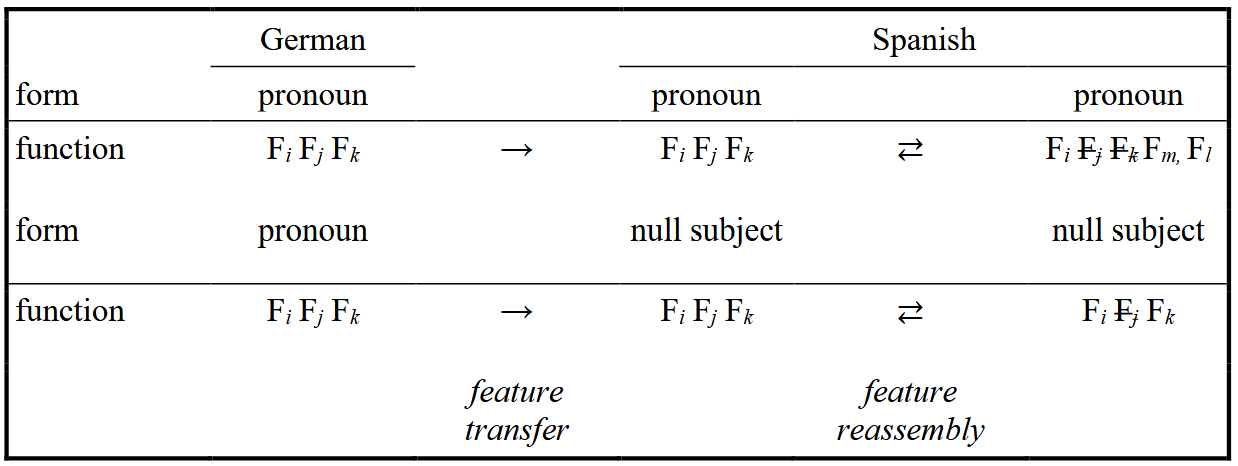
\includegraphics[keepaspectratio,alt={Scheme comparing subject realisation in German and Spanish in the context of feature transfer and feature reassembly. For German, the development from a pronoun with the functions Fᵢ, Fⱼ, Fₖ to a pronoun is shown. For Spanish, pronouns and null subjects are compared, each with the functions Fᵢ, Fⱼ, Fₖ. Arrows illustrate feature transfer from German to Spanish, as well as bidirectional feature reassembly, whereby some functions of a form in L1 can be transferred to L2 in the same way. In the course of second language acquisition, some functions have to be reassembled and must therefore be relearned, as the L2 form can have different functions to those in the L1.}]{images/Kocher_Feature-Reassembly.png}}

}

\caption{\label{fig-feature-reassembly1}Schematic application of feature
transfer and feature reassembly to L1 German pronoun use (from
\citeproc{ref-kocher_subject_2025}{Kocher, 2025}: 26).}

\end{figure}%

The first stage of the proposed reassembly process involves transferring
the contexts in which pronouns are used in German to Spanish. Thus,
learners initially assume that Spanish pronouns are used in the same
contexts as their German equivalents, represented by the contexts
\emph{F}\textsubscript{i}, \emph{F}\textsubscript{j},
\emph{F}\textsubscript{k}. With increasing proficiency, learners
recognise the ``form-meaning mismatches''
(\citeproc{ref-dominguez_early_2022}{Domínguez and Arche, 2022}: 189)
between the two languages and gradually learn that Spanish pronouns are
appropriate in contexts such as \emph{F}\textsubscript{i},
\emph{F}\textsubscript{m} and \emph{F}\textsubscript{l}, but not in
\emph{F}\textsubscript{j}, \emph{F}\textsubscript{k}. The same process
applies to null subjects. Initially, learners transfer the contexts
associated with German pronouns to Spanish null subjects. With
increasing proficiency, they reassemble these form-meaning mappings and
learn that null subjects are appropriate in contexts such as
\emph{F}\textsubscript{i} and \emph{F}\textsubscript{k}, whereas another
subject form is required in \emph{F}\textsubscript{j}. Through this
``transfer and subsequent reassembly of features from L1 to L2
expressions'' (\citeproc{ref-kocher_subject_2025}{Kocher, 2025}: 9),
learners develop new form-meaning mappings.

The \emph{Feature-Reassembly Hypothesis} has also been applied to L1
English learners of Spanish, for instance by Phinney
(\citeproc{ref-phinney_pro-drop_1987}{1987}: 229) and Domínguez and
Arche (\citeproc{ref-dominguez_early_2022}{2022}). Cho and Slabakova
(\citeproc{ref-cho2014}{2014}: 8) further propose that the acquisition
of functional features varies in difficulty depending on how those
features are realised in the L1 and L2 (see
Figure~\ref{fig-feature-reassembly2}).

\begin{figure}

\centering{

\pandocbounded{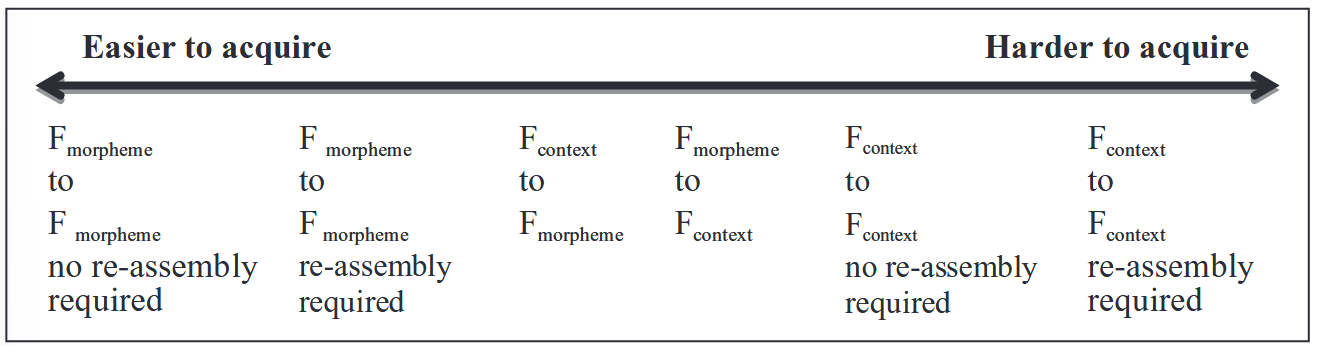
\includegraphics[keepaspectratio,alt={A horizontal continuum ranging from "Easier to acquire" on the left to "Harder to acquire" on the right. It presents six combinations of feature mappings and the corresponding need for feature reassembly: Fₘₒᵣₚₕₑₘₑ to  Fₘₒᵣₚₕₑₘₑ with no reassembly required; Fₘₒᵣₚₕₑₘₑ to Fₘₒᵣₚₕₑₘₑ with reassembly required; F𝚌ₒₙₜₑₓₜ to  Fₘₒᵣₚₕₑₘₑ; Fₘₒᵣₚₕₑₘₑ to F𝚌ₒₙₜₑₓₜ; F𝚌ₒₙₜₑₓₜ to F𝚌ₒₙₜₑₓₜ with no reassembly required; and F𝚌ₒₙₜₑₓₜ to F𝚌ₒₙₜₑₓₜ with reassembly required. The diagram represents increasing acquisition difficulty depending on the type of feature mapping and whether feature reassembly is necessary.}]{images/Feature-Reassembly2.png}}

}

\caption{\label{fig-feature-reassembly2}Cline of difficulty in
functional feature acquisition in various learning situations, adapted
in Cho and Slabakova (2014: 8)}

\end{figure}%

The easiest features to acquire are those that are explicitly or
morphologically expressed in the L1 and are likewise expressed
morphologically in the L2, as these do not require reassembly. More
difficult are features that are expressed only contextually in the L1
but morphologically in the L2. Conversely, morphologically expressed
features in the L1 that are expressed only contextually in the L2 are
even more difficult to acquire. The most difficult cases involve
features that are expressed only contextually in both languages but
nevertheless require reassembly. The following section applies these two
theoretical approaches to L1 German and L1 English learners and reviews
previous research on subject realisation in L2 Spanish prior to Kocher
(\citeproc{ref-kocher_subject_2025}{2025}).

\subsubsection{Subject realisation by L1 English and L1 German learners
of L2 Spanish}\label{priorresearch-resumee}

Given the low target-likeness of pronoun use, even among advanced
learners, pronoun reassembly remains difficult, as learners seem to
transfer the L1 use of pronouns to L2 Spanish in the vast majority of
cases (see \citeproc{ref-kocher_subject_2025}{Kocher, 2025}: 26;
\citeproc{ref-casteele_exploratory_2020}{Casteele and Palomares Ortiz,
2020}: 443). The only target-like pronoun use identified by Kocher
occurred in topic shift contexts
(\citeproc{ref-kocher_subject_2025}{Kocher, 2025}: 26). At the same
time, even the less advanced learners showed almost target-like use of
null subjects and DPs. However, the L1 German data revealed an overuse
of null subjects in MCs with topic shifts and an overuse of DPs in SCs
with topic shifts, where Spanish native speakers would typically use
pronominal subjects (\citeproc{ref-kocher_subject_2025}{Kocher, 2025}:
25). Thus, although interface complexity contributes to difficulties in
L2 subject realisation, it cannot by itself account for the overuse of
null subjects and DPs predicted by the \emph{Interface Hypothesis}.
Kocher therefore argues that the \emph{Interface Hypothesis} should be
considered as intertwined with the \emph{Feature-Reassembly Hypothesis}.
Following the logic of both hypotheses, the results suggest that L1
German learners initially use more formally complex pronouns as a
``close functional match to Spanish null subjects''
(\citeproc{ref-kocher_subject_2025}{Kocher, 2025}: 26).

Similar difficulties have been observed among L1 English learners of
Spanish. In their story-retelling and paired-discussion study, Domínguez
and Arche found that acquisition difficulties also affect null subjects
at early stages and are therefore not restricted to overt subjects at
the syntax-pragmatics interface
(\citeproc{ref-dominguez_early_2022}{2022}: 217). Consequently, the
\emph{Interface Hypothesis} alone cannot account for the acquisition
difficulties observed in their data. They argue instead that L2
acquisition is shaped by feature reassembly in combination with
interface complexity, the choice of oral versus written tasks, and
learners' overall oral production proficiency
(\citeproc{ref-dominguez_early_2022}{Domínguez and Arche, 2022}: 217).

Prior to Kocher (\citeproc{ref-kocher_subject_2025}{2025}) and Domínguez
and Arche (\citeproc{ref-dominguez_early_2022}{2022}), Liceras and Díaz
(\citeproc{ref-liceras_topic-drop_1999}{1999}) investigated subject
acquisition in spoken data from three L1 German speakers and briefly
discussed subject realisation in film-plot descriptions. Contrary to
their expectation that null subjects would be more frequent in MCs than
in SCs, the three L2 participants used null subjects more frequently in
SCs, diverging from the Spanish native speakers in their study
(\citeproc{ref-liceras_topic-drop_1999}{Liceras and Díaz, 1999}: 32).
Overall, the body of research on the behaviour of L1 German learners is
relatively limited, whereas a broader research base has investigated
subject realisation among L1 English learners, particularly with regard
to variables such as referential (dis)continuity, contrast, and clause
type.

In their meta study, Casteele and Palomares Ortiz compare findings from
several studies investigating whether L1 English learners of L2 Spanish
interpret continuous subjects as null or overt subjects
(\citeproc{ref-casteele_exploratory_2020}{2020}: 444). Their comparison
shows that intermediate learners in Rothman and Iverson
(\citeproc{ref-rothman2007}{2007}) as well as Rothman
(\citeproc{ref-rothman_pragmatic_2009}{2009}) showed a strong preference
for interpreting both null and overt subjects as continuous, although
the proportion was higher for null subjects (84-92\%) than for overt
subjects (61-65\%). While the interpretation of null subjects as
continuous is consistent with native speaker patterns, the
interpretation of overt subjects diverges from native speaker results.
Native speakers interpreted 80\% of null subjects but only one third
(36\%) of overt pronouns as continuous (see
Section~\ref{sec-ReferentialContinuity}). The proportion of continuous
interpretations of overt subjects was even higher in the studies by
Keating et al. (\citeproc{ref-keating2011}{2011}) and Jegerski et al.
(\citeproc{ref-jegerski2011}{2011}). They found that L2 Spanish
learners, including advanced learners, assigned continuous
interpretations to overt subjects in 54-56\% of cases and to null
subjects in 60-61\% of cases. All of these findings are consistent with
Lozano's observation that even advanced L1 English learners tend to
overproduce overt subjects in continuous contexts where a null subject
would be pragmatically appropriate (\citeproc{ref-lozano2009}{Lozano,
2009}: 157).

Lozano further reports a smaller, non-significant tendency for learners
to underproduce overt subjects by using null subjects in topic shift
contexts (\citeproc{ref-lozano2009}{Lozano, 2009}: 157). A similar
pattern is found in the advanced L2 study by Clements and Domínguez,
whose learners ``over-accept null subjects and find it difficult to
reject them when an overt pronoun is preferred by the controls''
(\citeproc{ref-clements_reexamining_2016}{2016}: 1). Taken together,
these findings suggest that maintaining a topic may be more difficult
for L2 learners than signalling a topic shift. As Quesada summarises,
``topic-continuity contexts appear to be more problematic than topic
shift and contrastive focus contexts, at least in L2 Spanish''
(\citeproc{ref-quesada2020}{2020}: 960).

Clause type represents another potential source of cross-linguistic
influence. In German and English, null subjects are infrequent and
mainly restricted to MCs, whereas Spanish permits them in both MCs and
SCs (see \citeproc{ref-torres_cacoullos_variationist_2019}{Torres
Cacoullos and Travis, 2019}: 1). L1 German and English learners might
therefore be expected to transfer their L1 patterns and use null
subjects primarily in MCs. Kocher's results partly support this
expectation: like Spanish native speakers, L1 German learners used DPs
and null subjects mainly in MCs and pronouns mainly in SCs. However, L1
German learners significantly overused pronouns in MCs (40.8\%, \emph{N}
= 147) compared with the native speakers (26.5\%, \emph{N} = 22) (see
\citeproc{ref-kocher_subject_2025}{Kocher, 2025}: 17). This finding
contrasts with Liceras and Díaz, who found fewer null subjects in SCs
than in MCs among Spanish native speakers. This is a pattern also
observed among L1 English learners but not among the L1 German learners
in their study (\citeproc{ref-liceras_topic-drop_1999}{Liceras and Díaz,
1999}: 32). As Kocher notes, these inconsistent findings suggest that
subject type may depend more directly on other variables, such as
referential (dis)continuity and information structure, while clause type
may influence subject realisation only indirectly (see
\citeproc{ref-kocher_subject_2025}{Kocher, 2025}: 15).

\subsection{Research Questions}\label{research-questions}

This reproduction and close replication study addresses three research
questions:

\textbf{RQ1} examines whether the findings reported in Kocher
(\citeproc{ref-kocher_subject_2025}{2025}) are reproducible and robust.
Given that most of the code underlying Kocher's MuPDARF analysis is
publicly accessible through their
\href{https://osf.io/zr9wh/overview}{OSF} repository, the analysis is
expected to be reproducible using the CEDEL2 dataset.

\textbf{RQ2} examines the extent to which subject realisation differs
between L2 Spanish speakers of L1 German and English. Both learner
groups are expected to show broadly similar patterns of target-likeness,
as both start from a non-NSL background and therefore face the shared
demands involved in acquiring Spanish subject realisation. However,
differences may arise from the distinct subject-realisation systems of
the two L1s. In particular, English permits subject omission in a
limited range of discourse contexts, whereas subject omission in German
is more restricted and is rarely used in formal or written language. L1
English learners may therefore show different patterns of subject
omission and, consequently, different degrees of target-likeness
compared with L1 German learners.

\textbf{RQ3} investigates whether the gender of the L2 speakers and the
gender of the subject referents influence the target-likeness of subject
realisation and whether these gender-related variables interact with
other variables of subject realisation. Masculine human referents appear
to be more prominent in the CEDEL2 corpus, reflecting both the higher
number of human masculine referents compared with human feminine
referents and the tendency for human subjects to be predominantly
masculine. Therefore, masculine referents are expected to occur more
frequently in absolute terms and to be therefore realised in a more
heterogeneous manner by using overt and covert subjects. Furthermore,
following Da Cunha (\citeproc{ref-dacunha2024}{2024}), who reports a
masculine subject bias among both male and female speakers, masculine
subjects are expected to be predominantly realised by male L1 Spanish
speakers and potentially by L2 speakers as well. The following chapter
describes the data, methodology, and replication design used to address
these research questions.

\section{Methodology}\label{sec-Methodology}

The following methodology chapter presents the fourfold design of the
study, comprising (1) the reproduction of Kocher's original data and
analyses, (2) the robustness check of the annotation and L1 German
speaker results through dataset extension, (3) the close replication
extending the original model by adding gender as two new variables, and
(4) the further close replication applying the extended model to an L1
English speaker dataset. It introduces the CEDEL2 corpus, describes the
data selection and pre-processing, outlines the exclusion criteria and
annotation procedure, and explains the replication design, including the
concept of repetitive research and the statistical modelling approach.

\subsection{CEDEL2 Corpus}\label{sec-Corpus}

Kocher's study is based on narrative texts produced by native speakers
of Spanish and L2 learners of Spanish from the freely available
\emph{Corpus Escrito del Español como L2} (CEDEL2)
(\citeproc{ref-lozano_cedel2_2022}{Lozano, 2022}: 975;
\citeproc{ref-kocher_subject_2025}{Kocher, 2025}: 14). CEDEL2 is a
multi-first-language corpus comprising L2 learners of Spanish with
twelve different L1s across all proficiency levels
(\citeproc{ref-lozano_cedel2_2022}{Lozano, 2022}: 965). In addition, it
includes several native Spanish control subcorpora and data from
approximately 4400 speakers, amounting to more than 1,100,000 words in
total (\citeproc{ref-lozano_cedel2_2022}{Lozano, 2022}: 965). The corpus
consists primarily of written production data and contains additional
demographic metadata for each participant. The data were collected via
dedicated online forms (\citeproc{ref-lozano_cedel2_2022}{Lozano, 2022}:
974).

The data extracted for the present study stem from the \emph{Retell the
Chaplin} video task, which is particularly suitable for investigating
subject realisation and anaphora resolution in both native and L2
Spanish (see \citeproc{ref-lozano_cedel2_2022}{Lozano, 2022}: 971).
Participants were allowed to watch the video multiple times, and there
appears to have been no time limit for completing the task, with an
average completion time of 60.4 minutes
(\citeproc{ref-kocher_subject_2025}{Kocher, 2025}: 14). All participants
completed the same task, which limits the generalisability of the
findings beyond this particular elicitation context. However, as
recommended in contrastive interlanguage analysis (see
\citeproc{ref-granger2015}{Granger, 2015}: 9), comparing the data of
native speakers and L2 learners provides a precise and meaningful
contrast and thereby ensures maximum comparability
(\citeproc{ref-lozano_cedel2_2022}{Lozano, 2022}: 968). In addition to
completing the main production task, participants provided information
about their demographic and linguistic background and completed a
Spanish placement test (see \citeproc{ref-lozano_cedel2_2022}{Lozano,
2022}: 970).

The Spanish native speakers are mainly from different areas of Spain,
which may have affected the homogeneity of the L1 comparison group (see
\citeproc{ref-kocher_subject_2025}{Kocher, 2025}: 14). They are between
21 and 51 years of age (mean 34). The L1 German speakers are between 19
and 71 years of age (mean 26.1), whereas the L1 English speakers are
between 16 and 74 years of age (mean 25.5). Of all L1 German speakers,
77.8\% have lived abroad in a Spanish-speaking country, compared with
41.9\% of L1 English speakers.

\subsection{Data}\label{data}

\subsubsection{Data selection and
pre-processing}\label{sec-data-selection-prerocessing}

First, to ensure that Kocher's study results could be reproduced by
rerunning the original scripts with the original data, I used the
manually annotated data for native Spanish and L1 German speakers
available in the study's \href{https://osf.io/zr9wh/overview}{OSF}
repository, from which I also retrieved the R scripts underlying the
present reproduction study. The repository contains a \texttt{readme.md}
file providing an overview of the available files and data frames, as
well as brief information on the exclusion criteria, the key variables
included in the final model, the packages used, the analysis procedure,
and how to cite Kocher's scripts and data. In addition, it contains a
folder with the processed and annotated native and L1 German speaker
data, an R script for the descriptive analyses (see
\texttt{descriptive.R} in Appendix A), the MuPDARF analysis (see
\texttt{mupdarfanalysis.R} in Appendix A), and a further script in which
proficiency levels were calculated (see \texttt{demographics.R} in
Appendix A). The created figures were saved in a separate
\texttt{Figures} folder within the repository.

The main reason for using Kocher's L1 German speaker dataset rather than
extracting the data from CEDEL2 again is that the dataset had already
been pre-processed and manually annotated, thereby facilitating the
robustness check conducted later in the study. Although Kocher's L1
German dataset was based on the complete L1 German speaker dataset from
the \emph{Charlie Chaplin} task available in CEDEL2 at the time of their
study, the native Spanish speaker dataset used in the study was based
only on a selection of the available CEDEL2 data and contains 522
clauses.

After rerunning Kocher's scripts with the original L1 German and native
Spanish speaker data, I tested the robustness of Kocher's
(\citeproc{ref-kocher_subject_2025}{Kocher, 2025}) results by adding
more recent L1 German speaker data that had not yet been included in the
corpus at the time of Kocher's study. In total, I extracted 662 clauses
from 17 additional L1 German speakers from CEDEL2 on 31 March 2026. The
annotation filter criteria applied in CEDEL2
(\citeproc{ref-lozano_cedel2_2022}{Lozano, 2022}) are presented in
Table~\ref{tbl-corpuscriteria}.

\begin{longtable}[]{@{}ll@{}}
\caption{The corpus filter criteria for data extraction in CEDEL2. The
remaining categories that are adjustable with a slider stayed in default
mode selecting the full range.}\label{tbl-corpuscriteria}\tabularnewline
\toprule\noalign{}
Corpus Filter Criteria & Selection \\
\midrule\noalign{}
\endfirsthead
\toprule\noalign{}
Corpus Filter Criteria & Selection \\
\midrule\noalign{}
\endhead
\bottomrule\noalign{}
\endlastfoot
\textbf{Result Type} & Texts \\
\textbf{Subcorpus} & Learners of L2 Spanish \\
\textbf{Medium} & Written \\
\textbf{Task Title} & Chaplin \\
\textbf{Sex, Proficiency, Filename} & Any \\
\textbf{L1} & L1 German - L2 Spanish \\
\end{longtable}

Prior to the manual annotation, the newly added L1 German data and the
complete L1 English dataset were segmented into clauses. Following
Kocher's procedure, SCs were separated from their corresponding MCs and
presented in the subsequent row. Within the MCs, omitted SCs were
indicated by square brackets ({[}\ldots{]}).

The annotation procedure largely followed the methodology established by
Kocher in order to ensure comparability across datasets. However,
additional information is required for the variables \emph{NSLhome} and
\emph{NSLadditional}, as their creation is not explained in Kocher
(\citeproc{ref-kocher_subject_2025}{2025}). The variable \emph{NSLhome}
was created based on the information provided in the
\emph{Languages.spoken.at.home} column and indicates whether a
participant acquired an NSL in the home environment.
\emph{NSLadditional} was derived from the \emph{ForeignLanguage} column
and indicates whether participants learned an NSL later through formal
instruction or other means. For participants who had already acquired an
NSL at home, \emph{NSLadditional} was also coded as \emph{Yes},
reflecting their continued exposure to an NSL. For participants without
home exposure to an NSL, \emph{NSLhome} was coded as \emph{Yes} only if
they had subsequently learned an NSL. For example, in the newly added L1
German dataset, only one participant had learned Italian as an
additional language, whereas all remaining participants had learned only
English, a non-NSL.\footnote{The separate .qmd file in Appendix A (see
  0\_Preprocessing.qmd) provides a detailed description of the
  pre-annotation process.} Finally, I joined the pre-processed L1 German
dataset with the already annotated original L1 German data from Kocher
(\citeproc{ref-kocher_subject_2025}{2025}), resulting in a dataset of
2997 clauses.

To further assess the robustness of Kocher's annotation, I extracted a
sample of 118 clauses from three L1 German speakers. A seed was set (see
\citeproc{ref-reiter2025}{Reiter, 2025}) to ensure that the randomly
generated sample could be reproduced, and the selected clauses were
re-annotated (see Section~\ref{sec-RobustnessAnnotation} for the
results).

For the second close replication study comparing subject realisation in
L1 English learners of Spanish, I applied the same filter criteria used
for the L1 German data, changing only the learner group to ``L1 English
- L2 Spanish''. After extracting the dataset, I segmented it so that
each clause was displayed in a separate row. For this process, I used
the machine-based tools \emph{Meta Llama 3.3 70B Instruct} and
\emph{DeepSeek R1 Distill Llama 70B} via the University of Cologne's
academic cloud access. Subsequently, I added the \emph{NSLadditional}
and \emph{NSLhome} columns and selected a data sample of 1300 clauses.

\subsubsection{Exclusion criteria and data
annotation}\label{sec-data-annotation}

The annotation procedure largely followed the methodology established by
Kocher (\citeproc{ref-kocher_subject_2025}{2025}) in order to ensure
comparability across datasets, while introducing a number of additional
exclusion criteria. In general, Kocher included only sentences with
referential subjects, that is, declarative and interrogative sentences
containing a referential subject. Imperative verb forms (e.g.~example
27) and impersonal constructions, such as indefinite \emph{se}
constructions (e.g.~example 28) or impersonal sentences (e.g.~example
29), were excluded and the corresponding clauses were deleted (see
\citeproc{ref-kocher_subject_2025}{Kocher, 2025}: 15). I decided to not
only omit these cases from the annotation, but also to delete the
excluded clauses, to prevent them from being selected by accident in the
random sample used for the L1 English data analysis. Impersonal forms
such as example 30, by contrast, were retained because they do not
contain imperative forms.

\begin{quote}
\begin{enumerate}
\def\labelenumi{\arabic{enumi}.}
\setcounter{enumi}{26}
\item
  \emph{{[}\ldots{]} que dice ``por favor ama y cuida ese huérfano''\\
  `\emph{{[}\ldots{]} which says, ``Please love and look after that
  orphan''}'}\\
  (datal2german, DE\_WR\_43\_29\_7\_14\_KP, excluded)
\item
  \emph{En el video se ve un hombre\\
  `\emph{In the video, you can see a man}'}\\
  (datal2german, DE\_WR\_30\_28\_2\_14\_GV, excluded)
\item
  \emph{Hay un inffantil}\\
  `There is a kid'\\
  (datal2english, EN\_WR\_14\_23\_1\_14\_B, excluded)
\item
  \emph{y le arrojaron basura\\
  `\emph{and they threw rubbish at him}'}\\
  (datal2english, EN\_WR\_21\_19\_2\_14\_JB, ID35\_2)
\item
  \emph{{[}\ldots{]} que dice: {[}Please love and take care of this
  orphan Child.{]}\\
  '}{[}\ldots{]} which says: {[}Please love and look after this orphaned
  child.{]}'\\
  (datal2german, DE\_WR\_27\_19\_1\_14\_AB, ID9\_28)
\end{enumerate}
\end{quote}

Clauses containing English direct speech were excluded but not deleted
entirely, as illustrated in example 31, whereas Spanish direct speech
was retained {[}see also example 27 above{]}. In addition, clauses
without a verb (e.g.~example 32), clauses containing English lexical
items within otherwise Spanish utterances (e.g.~example 33), and clauses
in which the intended verb could not be identified (e.g.~example 34)
were excluded from the annotation.

\begin{quote}
\begin{enumerate}
\def\labelenumi{\arabic{enumi}.}
\setcounter{enumi}{31}
\tightlist
\item
  \emph{¿Quizás la madre de otra bebé?\\
  `\emph{Perhaps the mother of another baby?}'}\\
  (datal2english, EN\_WR\_32\_59\_1\_14\_TC, excluded)
\item
  \emph{La cop chase the el hombre\\
  `\emph{The cop chases the man}'}\\
  (datal2english, EN\_WR\_12\_30\_0.7\_14\_NC, excluded)
\item
  \emph{Entonces el hombre montanió el bebé\\
  `\emph{Then the man picked up the baby}'}\\
  (datal2english, EN\_WR\_30\_20\_3\_14\_BRB, excluded)
\end{enumerate}
\end{quote}

Furthermore, meta-commentaries and first-person statements expressing
personal opinions were annotated as \emph{1st\_person} and removed from
the newly added L1 German and the complete L1 English datasets before
annotation in order to prevent their inclusion in the randomly selected
samples. Occurrences in Kocher's originally annotated clauses were
retained to preserve the original dataset for the reproduction study but
were excluded from the inferential statistical analysis. These cases
include comments referring to the task itself, such as example 35, as
well as first-person singular or plural reflections, as illustrated in
examples 36 and 37. Such clauses were excluded because they were too
infrequent to permit reliable analyses of first-person subject
expression or meaningful statistical interpretation. In contrast, Kocher
(\citeproc{ref-kocher_subject_2025}{2025}) generally removed such
clauses only after assigning ID numbers, resulting in gaps in the
annotated dataset. Their exclusion was also not applied consistently,
however, as a small number of first-person clauses remain in Kocher's
annotated dataset (e.g.~example 38) and consequently entered their
statistical analyses.

\begin{quote}
\begin{enumerate}
\def\labelenumi{\arabic{enumi}.}
\setcounter{enumi}{34}
\tightlist
\item
  \emph{{[}\ldots{]} pero {[}la película{]} es muy bueno\\
  `\emph{but {[}the film{]} is really good}'}\\
  (datal2english, EN\_WR\_14\_23\_1\_14\_BB, excluded)
\item
  \emph{I do not know what else to write.}\\
  (datal2english, EN\_WR\_20\_21\_4\_14\_PKO, excluded)
\item
  \emph{Al inicio del short lo vemos vestido mal con la ropa
  desarreglada\\
  `\emph{At the start of the short film, we see him dressed badly, with
  his clothes in disarray}'}\\
  (datal2english, EN\_WR\_39\_62\_2\_14\_MA, excluded)
\item
  \emph{Nunca aprendí español\\
  `\emph{I never learnt Spanish}'}\\
  (kocher\_germanL1\_data, DE\_WR\_20\_50\_2\_14\_HO, ID35\_2)
\end{enumerate}
\end{quote}

After applying Kocher's exclusion criteria, the final L1 German dataset
used for the robustness check and the first close replication contained
2863 clauses, whereas the L1 English dataset consisted of 1260 clauses.
The next step was the manual annotation of the data. I followed Kocher's
annotation scheme and extended it by adding the two gender-related
variables \emph{SpeakerGender} and \emph{SubjectGenus} (see
Table~\ref{tbl-variables}). The variables included in the annotation are
summarised below.

\begin{longtable}[]{@{}
  >{\raggedright\arraybackslash}p{(\linewidth - 2\tabcolsep) * \real{0.3307}}
  >{\raggedright\arraybackslash}p{(\linewidth - 2\tabcolsep) * \real{0.6693}}@{}}
\caption{Variables with annotated values included in Kocher's final
model, as well as the extended variables \emph{SpeakerGender}, extracted
from Kocher (\citeproc{ref-kocher_subject_2025}{2025}: 15) as well as
\emph{SubjectGenus}.}\label{tbl-variables}\tabularnewline
\toprule\noalign{}
\begin{minipage}[b]{\linewidth}\raggedright
Variables
\end{minipage} & \begin{minipage}[b]{\linewidth}\raggedright
Annotated values
\end{minipage} \\
\midrule\noalign{}
\endfirsthead
\toprule\noalign{}
\begin{minipage}[b]{\linewidth}\raggedright
Variables
\end{minipage} & \begin{minipage}[b]{\linewidth}\raggedright
Annotated values
\end{minipage} \\
\midrule\noalign{}
\endhead
\bottomrule\noalign{}
\endlastfoot
\textsc{\textbf{SubjectType}} & nullsub, dp, pron \\
\textsc{\textbf{SubjectPosition}} & PRE, POST, NA (for nullsub) \\
\textsc{\textbf{ClauseType}} & MC, SC \\
\textsc{\textbf{InformationStructure}} & GI(VEN), NE(W), NA \\
\textsc{\textbf{ReferentialContinuity}} & Y(ES), N(O), NA \\
\textsc{\textbf{(Proficiency)Score}} & 0-100 \\
\textsc{\textbf{Verb}} & verb of each clause \\
\textsc{\textbf{VerbConstruction}} & simple-finite, periphrasis-lexical,
periphrasis-gerund, modal, infinitive, passive \\
\textsc{\textbf{SpeakerGender}} & binary distinction: male, female \\
\textsc{\textbf{SubjectGenus}} & masc, fem, (unknown, 1st\_person) \\
\end{longtable}

The annotation includes nine explanatory variables, following Kocher
(\citeproc{ref-kocher_subject_2025}{2025}: 15-18), with
\emph{SpeakerGender} and \emph{SubjectGenus} added for the present
study. \emph{SubjectType} represents the formal realisation of the
subject and distinguishes between null subjects (\emph{nullsub}),
pronouns (including personal, demonstrative, relative, interrogative,
and \emph{wh}-pronouns, encoded as \emph{pron}), and full determiner
phrases or proper names (\emph{dp}). \emph{SubjectPosition} encodes the
position of overtly realised subjects relative to the finite verb,
distinguishing between preverbal (\emph{PRE}) and postverbal
(\emph{POST}) subjects. \emph{ClauseType} classifies each separated
clause as either a MC or a SC.

\emph{InformationStructure} distinguishes between new (NE), when a
referent is introduced into the discourse for the first time, and given
(GI), when the referent has already been mentioned. When the subject is
not identifiable, \emph{NA} is assigned. Rather than annotating the
(dis)continuity of a referent at the discourse or text level,
\emph{ReferentialContinuity} considers only the relation to the
preceding sentence. Kocher distinguishes between continuous referents
(Y{[}ES{]}), whose antecedent is the subject of the preceding sentence,
and discontinuous referents (N{[}O{]}), whose antecedent is not. When
the subject is not identifiable, \emph{NA} is assigned.

\emph{(Proficiency)Score} measures the language proficiency of the L2
speakers included in the analysis. It is based on the participants'
performance on a standardised language proficiency test and is reported
as a score ranging from 0 to 100, corresponding to the percentage of
correctly answered test items (see
\citeproc{ref-lozano_cedel2_2022}{Lozano, 2022}: 969). \emph{Verb}
identifies the predicate of the clause with which the subject agrees in
gender and number. \emph{VerbConstruction} classifies the predicate into
one of six categories: \emph{simple-finite}, \emph{periphrasis-lexical},
\emph{periphrasis-gerund}, \emph{modal}, \emph{infinitive}, and
\emph{passive}.

\emph{SpeakerGender} indicates the binary social gender reported by the
participants and recorded in the CEDEL2 corpus metadata. In addition, I
added the columns \emph{Textnr}, \emph{Sentence}, and \emph{ID}.
\emph{SpeakerGender} had already been annotated in Kocher's dataset but
was not included in the final model. \emph{SubjectGenus} encodes the
grammatical gender of the subject and distinguishes between the values
\emph{masc}, \emph{fem}, \emph{unknown}, and \emph{1st\_person}. The
latter two were excluded from the descriptive and inferential statistics
because their total number of occurrences is small and they do not
contribute to the interpretability of the plots. The variable does not
further distinguish between third-person singular and third-person
plural subjects. Further, the category \emph{unknown} includes cases in
which the subject cannot be clearly identified from the preceding
context or in which an impersonal form is used, as illustrated in
examples 39-41.

\begin{quote}
\begin{enumerate}
\def\labelenumi{\arabic{enumi}.}
\setcounter{enumi}{38}
\item
  \emph{Cuando de repente le tiran basura\\
  `\emph{When rubbish is suddenly thrown at him}'}\\
  (datal2german, DE\_WR\_41\_44\_30\_14\_AD, ID98\_3)
\item
  \emph{Por siguiente, se cae algo de arriba\\
  `\emph{Next, something falls from above}'}\\
  (datal2german, DE\_WR\_27\_21\_7\_14\_SG, ID11\_3)
\item
  \emph{que alguien se olvide {[}\ldots{]} el bebe\\
  `\emph{that someone forgets {[}\ldots{]} the baby}'}\\
  (datal2german, EN\_WR\_28\_20\_7.5\_14\_EC, ID61\_3)
\end{enumerate}
\end{quote}

Apart from these variables, Kocher states that they systematically
tested the ``impact of demographic (and other) {[}variables{]}'' when
determining the final models, but that ``{[}t{]}he models including
these variables were not superior on goodness-of-fit measures nor in
explanatory power, and therefore these variables are not included in the
final models'' (\citeproc{ref-kocher_subject_2025}{Kocher, 2025}: 15).
Neither the paper nor the scripts specify which variables were
originally planned for inclusion in the study. It is possible that
knowledge of an additional NSL, represented by the \emph{NSLadditional}
column, was among the variables that Kocher originally planned to
integrate into the analysis and subsequently excluded, as ``the
distribution of subject types does not differ significantly between the
speakers who know an additional NSL, and those who do not''
(\citeproc{ref-kocher_subject_2025}{Kocher, 2025}: 14).

Furthermore, the variable \emph{Specificity}, which was included in
Kocher's annotation scheme, was not incorporated into the final model. I
therefore decided not to annotate it in the L1 English data. Finally,
the variable \emph{SentenceType}, which likewise did not enter the final
model, is neither explained in the paper nor in the scripts. It was not
included in Kocher's final model, therefore it was also not annotated in
the L1 German data extension or the L1 English dataset. The challenges
involved in applying another author's annotation scheme and rerunning
their analysis scripts are discussed in the results section (see
Section~\ref{sec-Results}).

\subsection{Replication design}\label{sec-replication-design}

\subsubsection{Repetitive research}\label{sec-repetitive-research}

Repetitive research (\citeproc{ref-schuxf6ch2023}{Schöch, 2023}: 373)
refers to the research practice of re-examining previously tested
hypotheses using the same data and/or analysis methods as the original
studies. As this is a relatively recent area of research that is being
explored across a range of fields, including linguistics, psychology,
marketing, computer science, and second language acquisition research
(see \citeproc{ref-ruxf6seler2025}{Röseler et al., 2025}: 8), there are
almost as many definitions of reproducibility and replication (see
\citeproc{ref-voelkl2025}{Voelkl et al., 2025};
\citeproc{ref-barba2018}{Barba, 2018}) as there are fields investigating
them. It is therefore necessary to clarify the terminology used in the
present study.

First, I examine \textbf{computational reproducibility} following
Stodden's (\citeproc{ref-stodden2014}{2014}) approach. Computational
reproducibility refers to ``making computational environments available
for replication purposes'' and involves providing ``information about
codes, softwares, hardwares and implementation used'' (see
\citeproc{ref-theturingwaycommunity2025}{The Turing Way Community,
2025}). For the present study, I use a Microsoft Surface Pro 9 running
Windows 11 x64 (build 26200), with R version 4.6.0 (2026-04-24 ucrt,
called \emph{Because it was There}) and RStudio version 2026.07.1.
Kocher's original code, which I use for the reproduction and robustness
check (see folders \texttt{1\_Reproduction\_Kocher} and
\texttt{2\_Robustness\_Check}), as well as the adapted scripts
containing the model extension and analyses of the L1 English and L1
German datasets (see folders \texttt{3\_Extension1\_GenderGenus} and
\texttt{4\_Extension2\_EnglishGenus}), are provided in Appendix A.

In addition, \textbf{statistical reproducibility} ``repeat{[}s{]}
results for validation purposes'' (\citeproc{ref-stodden2014}{Stodden,
2014}) and therefore requires detailed information ``about the choice of
statistical tests, model parameters, and threshold values''
(\citeproc{ref-theturingwaycommunity2025}{The Turing Way Community,
2025}). Further information on the statistical analysis of Kocher
(\citeproc{ref-kocher_subject_2025}{2025}) is provided separately in
Section~\ref{sec-statistical-modelling}. \textbf{Inferential
reproducibility}, by contrast, refers to drawing ``qualitatively similar
conclusions from either an independent replication of a study or a
reanalysis of the original study'' (\citeproc{ref-goodman2016}{Goodman
et al., 2016}: 4). This distinction is particularly relevant because
different investigators may draw different conclusions from the same
statistical results. The inferential reproducibility of the present
study is addressed in the discussion (see Section~\ref{sec-Discussion}).

In addition to these dimensions of reproducibility, research
distinguishes between results that are \textbf{reproducible},
\textbf{replicable}, \textbf{robust}, and \textbf{generalisable}.
Following Le Foll (\citeproc{ref-lefoll2026}{2026}: 316), I adopt the
terminology proposed by The Turing Way Community
(\citeproc{ref-theturingwaycommunity2025}{2025}) to define these
concepts as they apply to the present study (see
Figure~\ref{fig-theturingway}).

\begin{figure}

\centering{

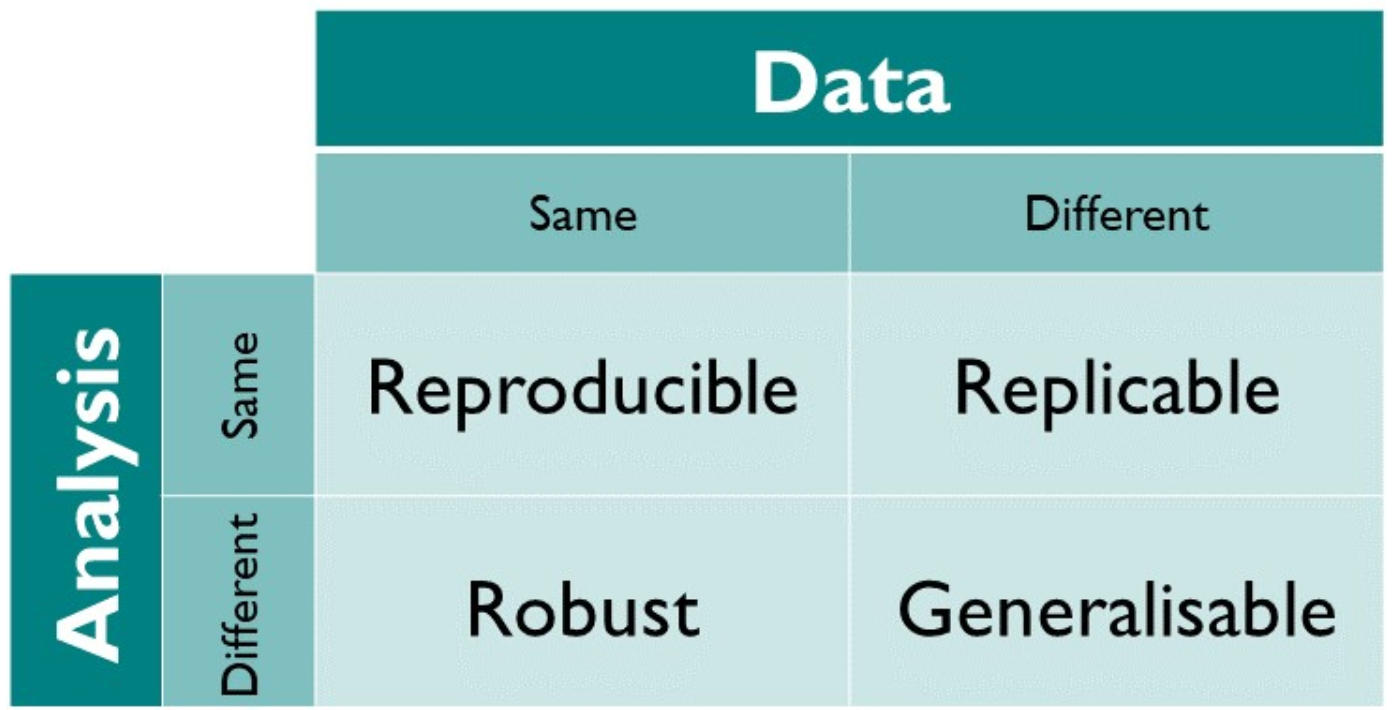
\includegraphics[width=3.15625in,height=\textheight,keepaspectratio,alt={Overview of how The Turing Way defines reproducible research, presented as a 2×2 matrix. The horizontal axis is Data, with columns labeled Same and Different. The vertical axis is Analysis, with rows also labeled Same and Different. The four outcomes are: Reproducible (same data, same analysis), Replicable (different data, same analysis), Robust (same data, different analysis), and Generalisable (different data, different analysis).}]{images/theturingway_repro.png}

}

\caption{\label{fig-theturingway}The Turing Way's definition of
reproducible research (The TuringWayCommunity CC BY 4.0)}

\end{figure}%

The first part of the present study constitutes a \textbf{reproduction}
study, as Kocher's original L1 German dataset is analysed using the same
analysis steps and scripts. A \textbf{replication}, by contrast, uses
the same analysis steps on a different dataset and aims ``to confirm,
consolidate, and extend knowledge and understanding within empirical
fields of study by confronting existing claims and ideas using new
evidence'' (\citeproc{ref-mcmanus2024}{McManus, 2024}: 1302). McManus
(\citeproc{ref-mcmanus2024}{2024}) conceptualise replication as a
continuum ranging from \textbf{exact replication}, involving no major
changes or manipulation of variables, through \textbf{close
replication}, involving one major change, and \textbf{approximate
replication}, involving two major changes, to \textbf{conceptual
replication}, involving three major changes. They further argue that the
greater the manipulation of the original study design, the less
appropriate the resulting study becomes for confirming the results of
the original study (\citeproc{ref-mcmanus2024}{2024}: 1302).

The concept of \textbf{robustness} is additionally defined in
Figure~\ref{fig-theturingway} as a study in which ``the same dataset is
subjected to different analysis workflows to answer the same research
question {[}\ldots{]} and a qualitatively similar or identical answer is
produced'' (\citeproc{ref-theturingwaycommunity2025}{The Turing Way
Community, 2025}). \textbf{Generalisable} results, and
\textbf{generalisability} itself, are not achieved simply by applying
different analysis procedures to different datasets but by ``combining
replicable and robust findings''
(\citeproc{ref-theturingwaycommunity2025}{The Turing Way Community,
2025}). The following section describes how these concepts are
operationalised in the reproduction, replication, and robustness studies
conducted in the present study.

To assess the findability, accessibility, interoperability, and
reusability of Kocher's study, data, and scripts, I use Wilkinson et
al.'s (\citeproc{ref-wilkinson2016}{2016}: 4) \textbf{FAIR principles}
as a guiding framework. My evaluation of Kocher's study according to
these principles is presented in Section~\ref{sec-evaluation-FAIRness}.
To make my own study as \textbf{findable} and \textbf{accessible} as
possible, I share the datasets before and after annotation (the latter
is provided in the subfolder annotations in the \emph{data} folder), as
well as the analysis scripts in my
\href{https://github.com/TizianaIlie/Github_thesis_TizianaIlie}{Github
repository} (see also Appendix A). The numbered folders containing the
reproduction, replication, and robustness analyses provide the files and
data required to rerun the respective analyses. Folder
\texttt{1\_Reproduction\_Kocher} contains the original data used by
Kocher, the generated figures, and the \texttt{.R} scripts
(\texttt{descriptive.R}, \texttt{demographic.R},
\texttt{mupdarfanalysis.R}), together with adapted versions
(e.g.~\texttt{descriptive\_TI.R}) in which adjustments were required to
run the code on my system. The datasets and annotation schemes used for
the remaining analyses are stored in the separate \texttt{data} folder.

In addition to the original three \texttt{.R} scripts and the
\texttt{Figures} folder, \texttt{2\_Robustness\_Check} contains the
robustness analysis
(\texttt{RobustnessCheck\_inner\_annotator\_agreement.qmd}) of the
sample of three speaker texts that I re-annotated and for which I
calculated inter-annotator agreement (see
Section~\ref{sec-statistical-modelling}). Folder
\texttt{3\_Extension1\_GenderGenus} contains the corresponding
\texttt{.qmd} file with the extended analysis, including the additional
variables, as well as the figures generated from this analysis. Since
the same extended L1 German dataset is used in
\texttt{2\_Robustness\_Check} and \texttt{3\_Extension1\_GenderGenus},
there is no need to provide the \texttt{descriptive.R} and
\texttt{demographic.R} scripts again. These scripts are included in
\texttt{4\_Extension2\_GenusEnglish}, where they are required because
the analysis is based on a new L1 English dataset.

To ensure \textbf{interoperability}, I provide information about the
operating system and the R and RStudio versions, as well as the names
and versions of the packages used in the analyses. Finally, to make the
data and scripts \textbf{reusable}, I named the annotated datasets used
for the analyses \emph{datal2german} and \emph{datal2english}, allowing
the same scripts to be applied to other datasets containing L1 German
and L1 English data. In addition, each clause was assigned a unique ID
based on \emph{Textnr\_Sentence}, and most of Kocher's original column
and variable names were retained. Where columns were renamed, removed,
or added, the corresponding changes are explained in the scripts.
Finally, I commented on most of Kocher's and my own code lines to make
the purpose of the individual functions and analysis steps transparent.

\subsubsection{Statistic modelling}\label{sec-statistical-modelling}

\paragraph{MuPDARF and decision tree
models}\label{mupdarf-and-decision-tree-models}

The main inferential statistical analyses in Kocher's study are
implemented in the \texttt{MuPDARFanalysis\_TI.R} script.
\textbf{MuPDARF}, short for \emph{Multifactorial Prediction and
Deviation Analysis Using Regression/Random Forests}, is a ``multi-step
analysis procedure developed for learner corpus researcher''
(\citeproc{ref-kocher_subject_2025}{Kocher, 2025}: 18) that compares L1
and L2 data within a single multifactorial modelling framework. The
method quantifies the extent to which non-native speakers deviate from
the linguistic choices that native or reference speakers would be
expected to make in the same context (see
\citeproc{ref-griesdeshors2014}{Gries and Deshors, 2014}: 132). This
deviation is expressed through a measurable variable referred to as
\emph{reference-likeliness} or \emph{target-likeliness}. MuPDARF was
developed as an alternative to traditional regression- and tree-based
approaches and consists of four consecutive modelling steps (see
\citeproc{ref-griesdeshors2014}{Gries and Deshors, 2014}: 132), which
are illustrated for Kocher's study in Figure~\ref{fig-flowchart}.

\begin{figure}

\centering{

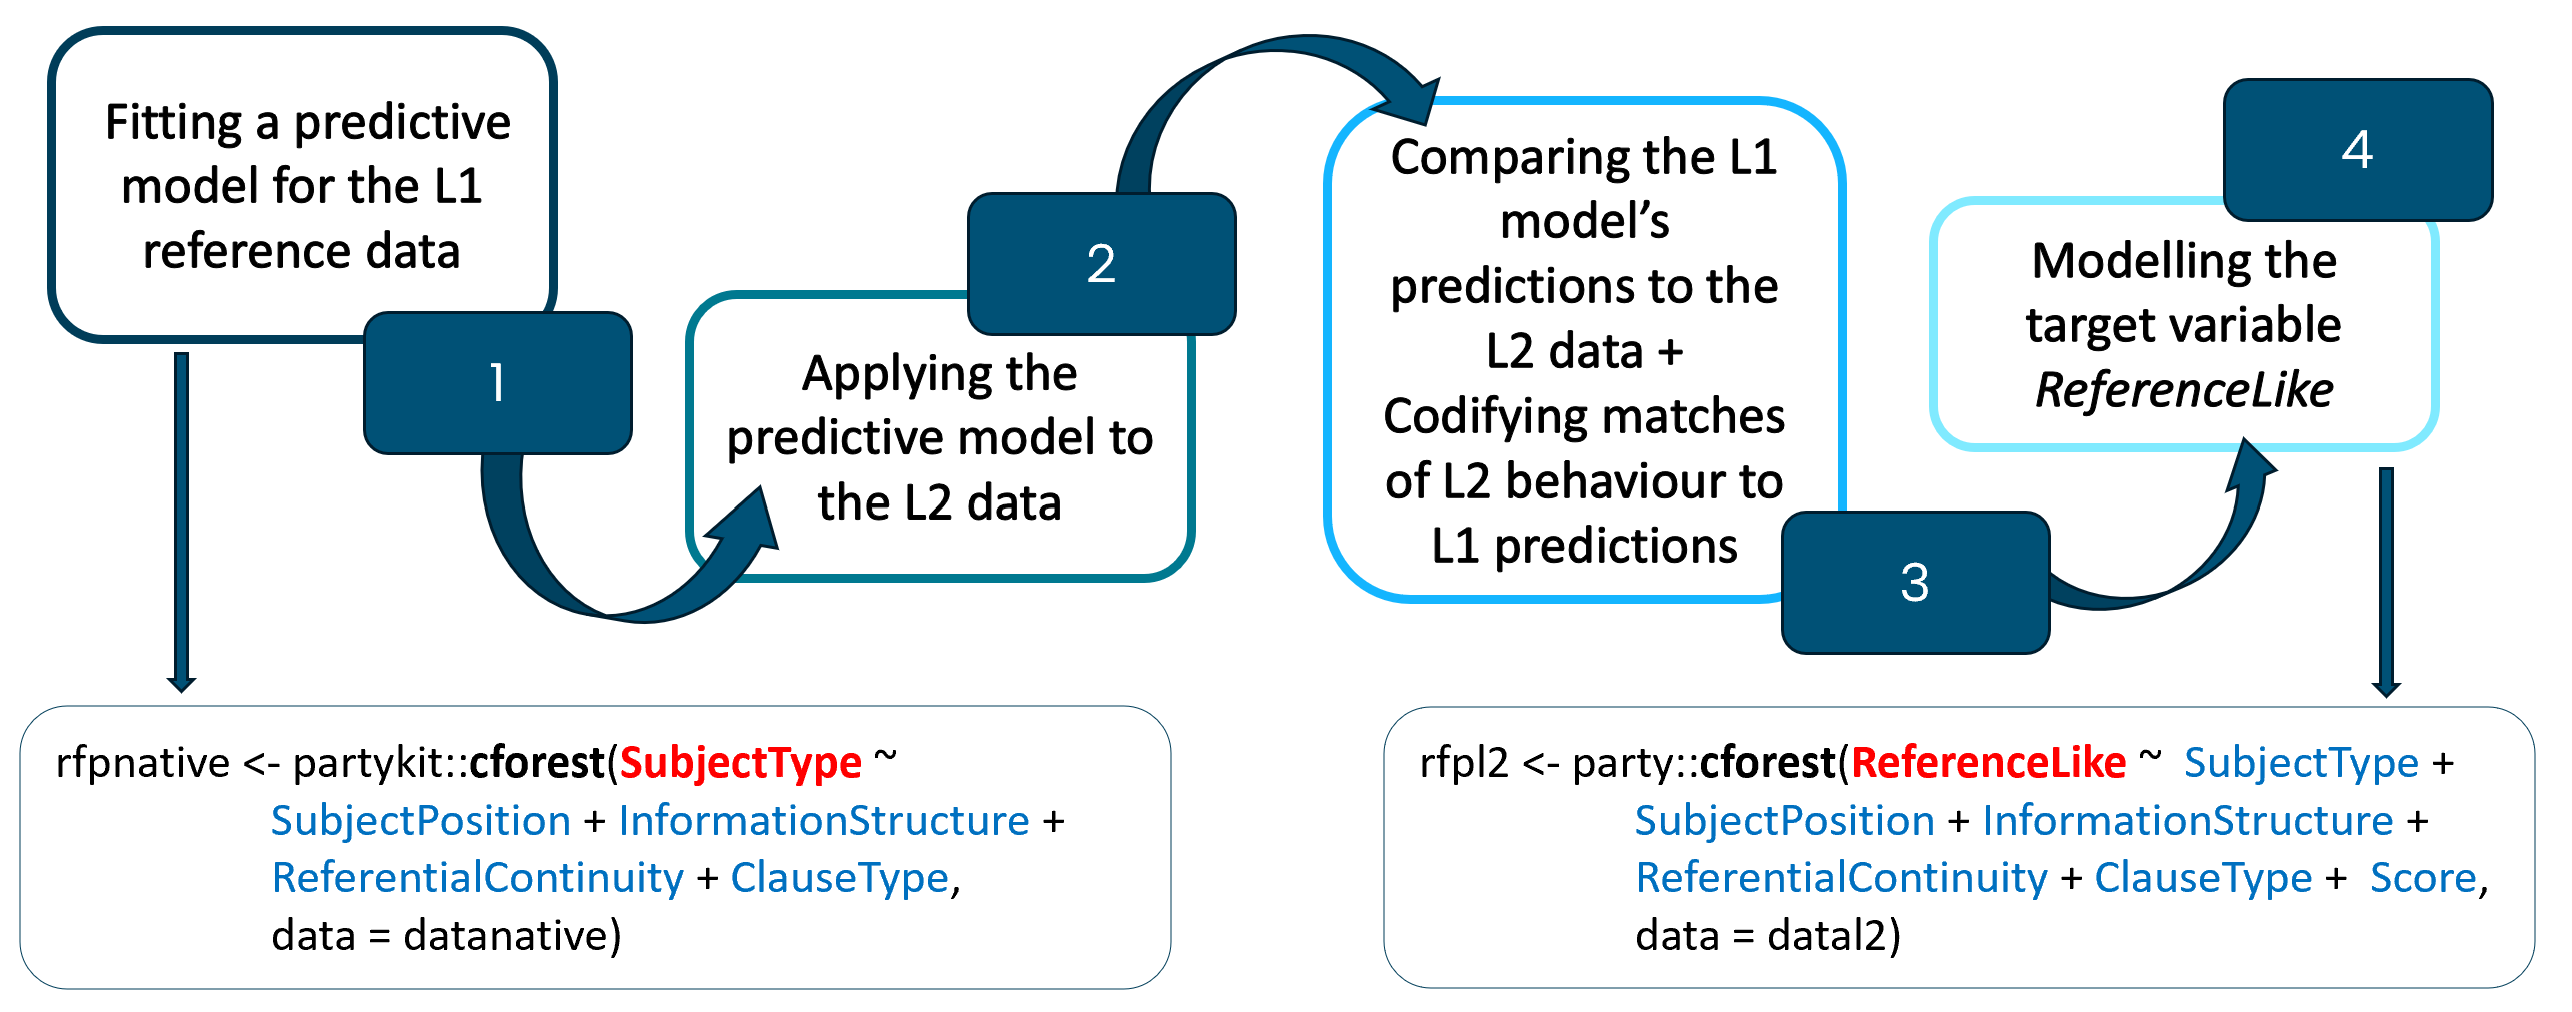
\includegraphics[width=6.89583in,height=\textheight,keepaspectratio,alt={Flowchart illustrating the four-step MuPDAR/F workflow: (1) train a predictive model on L1 reference data, (2) apply the model to L2 data, (3) compare L1 predictions with L2 observations to code whether L2 behavior matches native-speaker predictions (ReferenceLike), and (4) model the resulting ReferenceLike variable. Example cforest model codes for steps 1 and 4 are shown below the workflow containing all variables that entered into the model.}]{images/flowchart.png}

}

\caption{\label{fig-flowchart}Flowchart illustrating the four-step
MuPDARF workflow. Example cforest model codes for steps 1 and 4 are
shown below (CC-BY-NC-SA).}

\end{figure}%

In the first step, a predictive model is trained on the L1 data, which
serve as the reference dataset. In the second step, this model is
applied to the L2 data to predict the linguistic choice that a reference
speaker would most likely make in the communicative context of each
learner observation. The third step compares these predictions with the
observed learner productions and determines whether the learner made the
canonical choice predicted by the L1 model. Matches between the
predicted and observed forms are then encoded in a new variable,
\emph{ReferenceLike}. Finally, in the fourth step, this newly created
variable is modelled as the response variable in a second regression
model (compare \citeproc{ref-gries_theres_2020}{Gries et al., 2020}:
69).

To implement this procedure, Kocher uses random forests, or ``ensembles
of decision trees'' (\citeproc{ref-molnar_interpretable_2019}{Molnar,
2019}: 11), as the primary modelling technique. Decision trees
recursively partition the data by selecting, at each split, the
predictor variable most strongly associated with the response variable.
Through this recursive partitioning process, the data are divided into
increasingly homogeneous subsets until no further statistically
meaningful partitioning is possible (see
\citeproc{ref-kocher_subject_2025}{Kocher, 2025}: 19). In Kocher's
implementation, the individual trees are conditional inference trees
fitted using the \texttt{cforest()} function.

Random forests are widely used in machine learning and are particularly
suited to complex corpus-linguistic data because they combine the
predictions of hundreds of individual decision trees into a single
ensemble model. As ``blends of several models''
(\citeproc{ref-molnar_interpretable_2019}{Molnar, 2019}: 11), they
generally outperform individual decision trees and many alternative
modelling approaches. However, their complexity also makes them
difficult to interpret. Random forests are therefore commonly described
as ``black box models''
(\citeproc{ref-molnar_interpretable_2019}{Molnar, 2019}: 13), as they
cannot be readily visualised
(\citeproc{ref-gries_classification_2019}{Gries, 2019}: 5) and their
internal decision-making process is largely opaque to human
interpretation (\citeproc{ref-molnar_interpretable_2019}{Molnar, 2019}:
11).

A common approach to interpreting random forests, and the one adopted by
Kocher, is to calculate variable importance scores, which ``quantify the
size of the effect that a predictor has on the response''
(\citeproc{ref-gries_classification_2019}{Gries, 2019}: 5).
Nevertheless, variable importance provides only limited insight into the
structure of the underlying model, as Kocher also notes
(\citeproc{ref-kocher_subject_2025}{2025}: 20). To facilitate
interpretation, the study additionally employs surrogate modelling.

A surrogate decision tree is a simplified approximation of the
underlying random forest. Unlike a random forest, which consists of a
large ensemble of decision trees trained on random subsets of the data,
a surrogate model consists of a single decision tree trained on the
predictions of the underlying black-box model (see
\citeproc{ref-kocher_subject_2025}{Kocher, 2025}: 20). Although
considerably less complex, surrogate trees remain flexible while
offering a much higher degree of interpretability and can be easily
visualised (see \citeproc{ref-gries_classification_2019}{Gries, 2019}:
20). They therefore allow researchers to draw more intuitive conclusions
about the predictions and interaction patterns learned by the underlying
random forest model (see
\citeproc{ref-molnar_interpretable_2019}{Molnar, 2019}: 163, 166).

\paragraph{Modelling of the reproduction and replication
study}\label{modelling-of-the-reproduction-and-replication-study}

The present study begins with a computational reproduction of Kocher's
analysis in order to assess whether the reported results can be
reproduced by rerunning the original scripts on the original data. To
this end, Kocher's original R scripts were rerun without modification on
the original Spanish native speaker and L1 German learner datasets (see
Appendix A, folder \texttt{1\_Reproduction\_Kocher}). The reproduction
comprises three scripts. The \texttt{demographic.R} script calculates
the Spanish proficiency scores of the learners and assigns them to the
beginner, intermediate, or advanced proficiency groups (see
\citeproc{ref-kocher_subject_2025}{Kocher, 2025}: 14). The
\texttt{descriptive.R} script performs an exploratory analysis of the
data and calculates descriptive statistics prior to modelling. These
include the distribution of subject types according to whether learners
possess knowledge of an additional NSL (see
\citeproc{ref-kocher_subject_2025}{Kocher, 2025}: 14), as well as the
distribution of subject constructions in preverbal and postverbal
position, the latter being associated with the expression of focus (see
\citeproc{ref-kocher_subject_2025}{Kocher, 2025}: 15).

As described in the previous subsection, the principal inferential
analyses are implemented in the \texttt{MuPDARFanalysis\_TI.R} script.
In the first MuPDARF step, a conditional inference random forest is
trained on the native speaker data using the \texttt{cforest()} function
of the \{partykit\} package (version 1.2-27; see Hothorn and Zeileis
(\citeproc{ref-hothorn2015}{2015})), which employs conditional inference
trees as base learners (\citeproc{ref-hothorn2026}{Hothorn et al.,
2026}: 2). The model predicts \emph{SubjectType} from the explanatory
variables \emph{SubjectPosition}, \emph{InformationStructure},
\emph{ReferentialContinuity}, and \emph{ClauseType} (see
Figure~\ref{fig-flowchart}). Subsequently, the \texttt{varimp.cforest()}
function from the same package is used to calculate the variable
importance scores of the native speaker model
(\citeproc{ref-hothorn2026}{Hothorn et al., 2026}: 54). Model accuracy
is assessed by constructing a confusion matrix and using the
\texttt{predict()} function of the \{stats\} package, version 4.6.0
(\citeproc{ref-rcoreteam2026}{{Team and worldwide}, 2026}: 1347), to
calculate the proportion of correctly predicted observations relative to
the total number of predictions.

In the second MuPDARF step, the trained L1 model is applied to the L2
German learner dataset. During prediction, only the explanatory
variables included in the L1 model are supplied, namely
\emph{SubjectPosition}, \emph{ClauseType}, \emph{InformationStructure},
\emph{ReferentialContinuity} and \emph{(Proficiency)Score}, while the
observed values of the response variable, \emph{SubjectType}, remain
hidden (see \citeproc{ref-kocher_subject_2025}{Kocher, 2025}: 19). For
each learner observation, the model predicts the subject form that a
native speaker would most likely have produced in the same context,
namely a null subject, pronoun, or DP.

The third step compares the predicted and observed subject realisations.
Based on this comparison, Kocher creates the categorical variable
\emph{ReferenceLike}, which indicates whether a learner's production
matches the prediction of the native speaker model. Matching predictions
are labelled \emph{correct}, whereas mismatches are classified according
to the subject type predicted by the model (\emph{predictpron},
\emph{predictdp}, or \emph{predictnullsub}) (see
\citeproc{ref-kocher_subject_2025}{Kocher, 2025}: 19).

In the fourth step, \emph{ReferenceLike} serves as the response variable
in a second random forest model fitted to the L2 learner data. The
explanatory variables comprise \emph{SubjectType},
\emph{SubjectPosition}, \emph{InformationStructure},
\emph{ReferentialContinuity}, \emph{ClauseType}, and
\emph{(Proficiency)Score}. As shown in the code presented in
Figure~\ref{fig-flowchart}, Kocher fitted this model using the
\texttt{cforest()} function of the \{party\} package (version 1.3-20;
see Hothorn et al. (\citeproc{ref-hothorn2005}{2005})).

As in the first modelling step, Kocher calculated model accuracy,
inspected the predictions for pronouns, DPs, and null subjects, and
calculated the importance of the variables. Random forests are
non-parametric models and therefore ``do not make any distributional
assumptions about the population that the sample was drawn from. They
are relatively robust in cases of data scarcity, high variability of
data and collinearity of variables''
(\citeproc{ref-kocher_subject_2025}{Kocher, 2025}: 19). Kocher therefore
reports prediction accuracy and variable importance rather than
conventional assumption diagnostics. The native speaker model is
reported to have a ``moderate accuracy of 64\%''
(\citeproc{ref-kocher_subject_2025}{Kocher, 2025}: 20), whereas the
final L2 learner model achieves a prediction accuracy of 99\%
(\citeproc{ref-kocher_subject_2025}{Kocher, 2025}: 22). For the native
speaker model, Kocher additionally reports:

\begin{quote}
``An alternative model of the L1 data, containing more predictor
variables targeting a large range of potential linguistic factors and
also including demographic factors, only lead to an increase of accuracy
of 1\%. It is possible that additional linguistics factors are at play,
or that a larger dataset could lead to a higher accuracy''
(\citeproc{ref-kocher_subject_2025}{Kocher, 2025}: 20).
\end{quote}

To increase model interpretability, Kocher additionally uses a surrogate
decision tree generated with the \texttt{surro()} function from the
\{moreparty\} package (version 0.4.1; Robette
(\citeproc{ref-robette2025}{2025})). The resulting surrogate tree has an
R² of 0.94, which Kocher interprets as indicating a good fit to the
underlying random forest model
(\citeproc{ref-kocher_subject_2025}{Kocher, 2025}: 23).

Following the computational reproduction, two separate robustness checks
are conducted. First, the reliability of Kocher's annotation is assessed
using a sample of three speakers comprising 118 clauses. The
inter-annotator agreement between Kocher's original annotation and my
re-annotation of the same clauses is calculated using Cohen's K,
implemented in the \{irr\} package (version 0.84.1). The resulting
agreement values are interpreted according to the scale proposed by
Landis and Koch (\citeproc{ref-landiskoch1977}{1977}), see
Section~\ref{sec-RobustnessAnnotation}.

Second, the robustness of Kocher's reported results is assessed by
rerunning the three original scripts on the extended L1 German learner
dataset, while leaving the MuPDARF analysis unchanged. This allows the
original analysis to be tested on a larger L1 German dataset containing
participants who were not included in Kocher's study. I use the term
\emph{robustness} here in a broader sense than the definition provided
by The Turing Way Community
(\citeproc{ref-theturingwaycommunity2025}{2025}), which refers to
applying different analysis workflows to the same dataset. In the
present study, the robustness check instead examines whether the results
remain stable when the same analysis is applied to an extended dataset
containing additional participants.\footnote{Using the term
  \emph{robustness check} for repeating the same analysis with a
  slightly extended dataset is debatable, as it could also be viewed as
  a form of replication, because in the end the analysis remains the
  same. However, in my research, extending the dataset with a small
  number of additional data points primarily serves to assess the
  robustness of the results, rather than to replicate them using
  completely different data.}

Finally, \textbf{two close replication studies} are conducted. In the
first replication, \textsc{SpeakerGender} and \textsc{SubjectGenus} are
introduced as additional predictor variables into the model trained on
the extended L1 German learner dataset. In the second replication, this
extended model is applied to an L1 English learner dataset. This design
enables comparisons not only of the role of gender-related variables in
the production of subject forms by L1 German learners, but also of the
original and extended variable sets across two learner populations whose
L1s are both non-NSLs but differ in their subject-realisation systems.
As Röseler argues, ``reproduction and replication should always be
considered together and if possible, reproduction should come before
replication'' (\citeproc{ref-ruxf6seler2025}{2025}: 26). The present
study follows this sequence by first reproducing Kocher's original
analyses, then assessing the robustness of the findings through
annotation re-analysis and dataset extension, and finally extending the
model through two close replications.

\section{Results}\label{sec-Results}

This chapter presents the computational, statistical, and inferential
reproduction of Kocher's (\citeproc{ref-kocher_subject_2025}{2025})
original study, examines changes in the results obtained in the
robustness check (Section~\ref{sec-RobustnessCheck}), and reports the
results of applying the model containing the two gender-related
variables to the extended native and L1 German speaker data
Section~\ref{sec-close-repl1}. Finally, it compares the descriptive
statistics and model results of the extended native and L1 German
datasets with those of the L1 English dataset.

\subsection{Reproduction of Kocher
(2025)}\label{sec-results-reproduction}

\subsubsection{Descriptive statistics and demographic
variables}\label{descriptive-statistics-and-demographic-variables}

The proportions and frequencies reported in Kocher's descriptive
statistics tables (\citeproc{ref-kocher_subject_2025}{2025}: 16-17)
could be reproduced exactly. The only difference occurred in the
plotting of the \emph{(Proficiency)Score} variable, shown in
Figure~\ref{fig-scores-german-kocher}.

\begin{figure}

\centering{

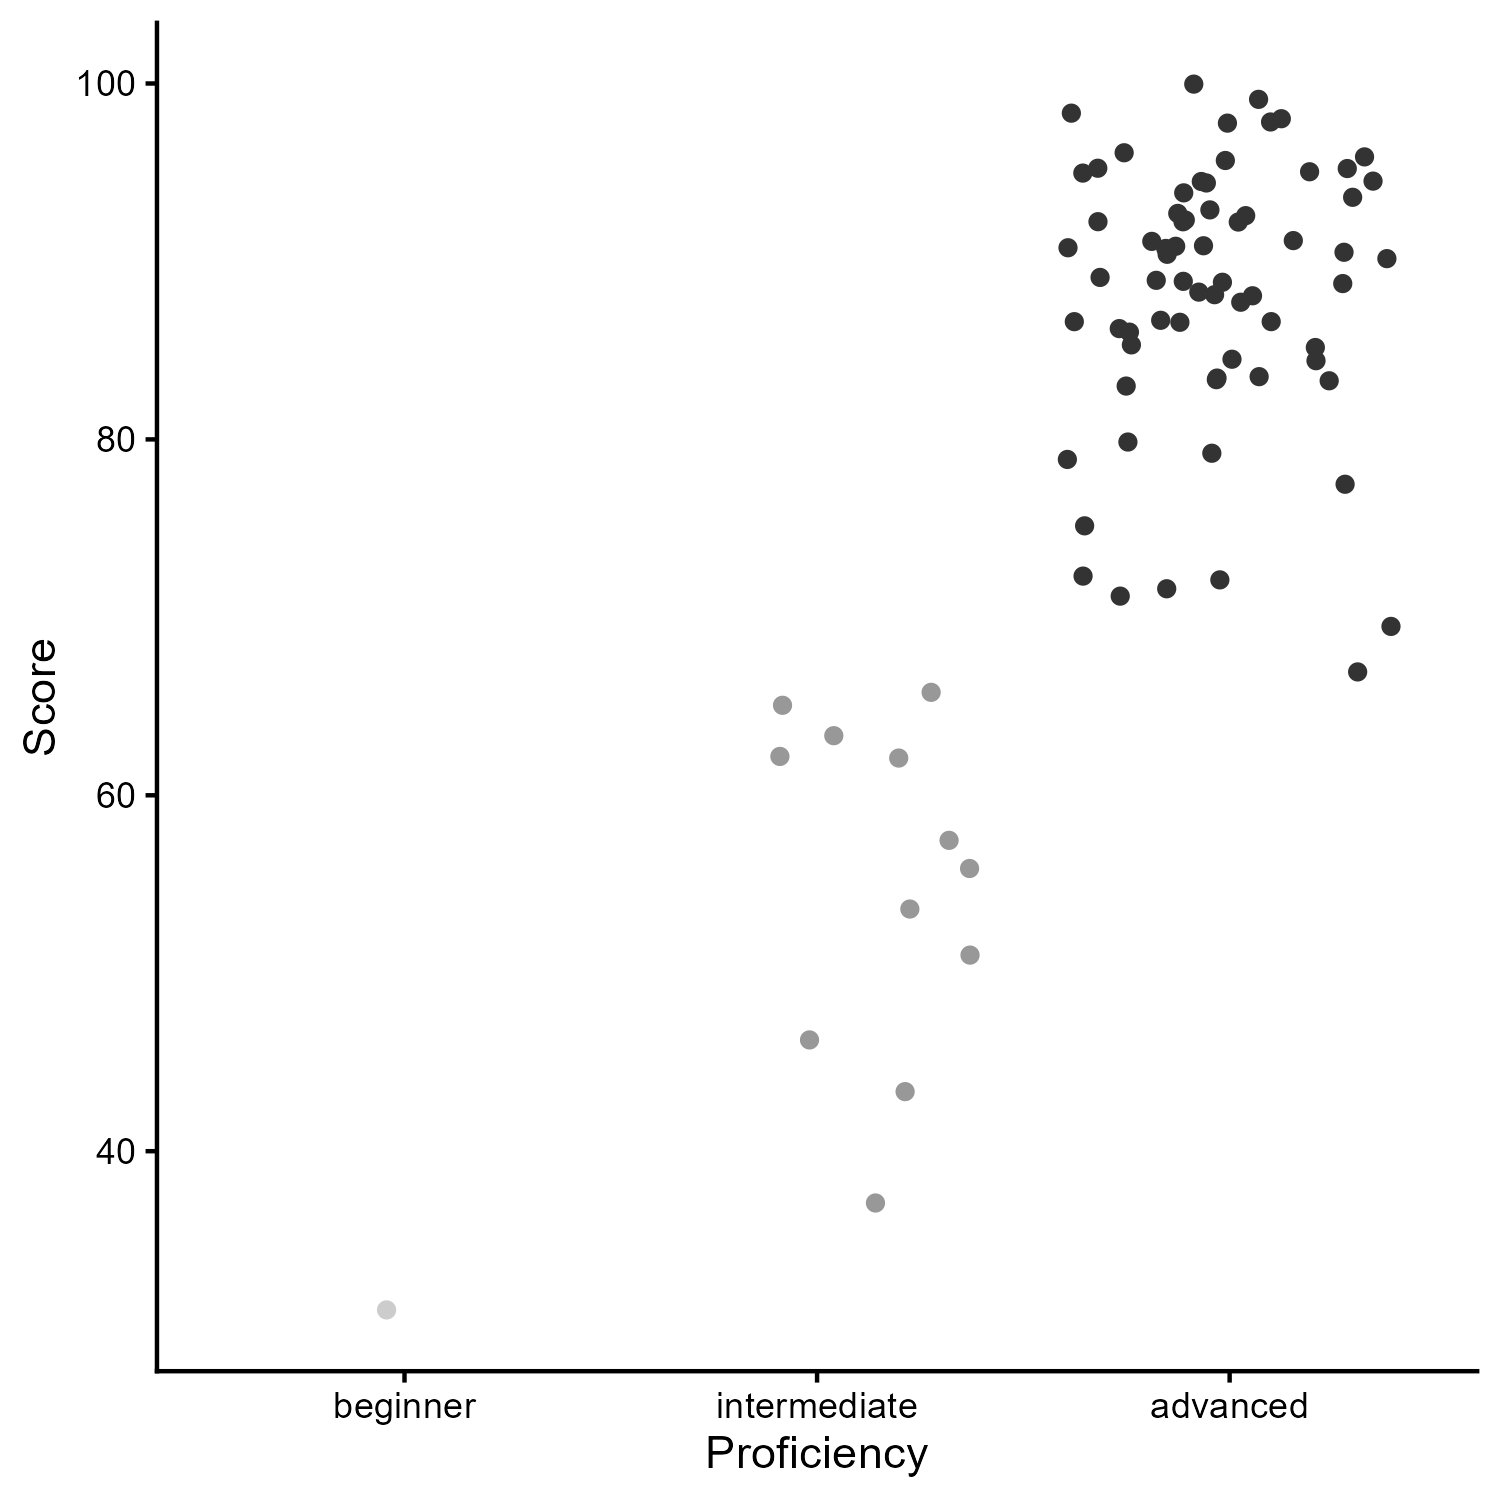
\includegraphics[width=2.60417in,height=\textheight,keepaspectratio,alt={This scatter plot shows the placement score of each L2 Spanish speaker by proficiency level. The x-axis shows three proficiency categories (beginner, intermediate and advanced), and the y-axis shows placement scores. Beginners are represented in light grey, with scores ranging from 1 to 33, while intermediate speakers are shown in grey, with scores ranging from 33 to 66. Advanced speakers are shown in black, with scores above 66. The plot clearly separates the three proficiency groups, with higher placement scores corresponding to higher proficiency levels, and it is strongly right-skewed given the larger number of advanced speakers.}]{1_Reproduction_Kocher/Analysis/Figures/scores.png}

}

\caption{\label{fig-scores-german-kocher}Placement score of each L2
speaker, light gray: beginners (\textless33), gray: intermediate
(33\textgreater66), black: advanced (\textgreater66).}

\end{figure}%

Although the distribution of the intermediate and advanced speakers is
plotted slightly differently in the original figure, the reproduced
figure conveys the same overall pattern: the L1 German learners of L2
Spanish are predominantly advanced. Only one speaker has a score below
33, while 12 speakers have scores between 33 and 66. The remaining 69
speakers have scores of 66 or higher (see also
\citeproc{ref-kocher_subject_2025}{Kocher, 2025}: 18). Of the 82
speakers, 18 have knowledge of an additional NSL. However, the
distribution of subject types does not differ significantly between
speakers who know an additional NSL and those who do not (X² = 1.7,
\emph{p} \textgreater{} 0.05) (compare
\citeproc{ref-kocher_subject_2025}{Kocher, 2025}: 14).

\subsubsection{Variable importance and model
accuracy}\label{varimp-repro}

The model accuracy of Kocher's native speaker model is 64\%, as stated
in the original study (\citeproc{ref-kocher_subject_2025}{2025}: 20).
The variable importance plot of Kocher's original native speaker model
(\citeproc{ref-kocher_subject_2025}{2025}: 21) is reproduced in
Figure~\ref{fig-varimp-natives-kocher}. It shows the same distribution
as the original figure, with \textsc{ReferentialContinuity} and
\textsc{InformationStructure} being by far the most influential
variables in the native speaker model.

\begin{figure}

\centering{

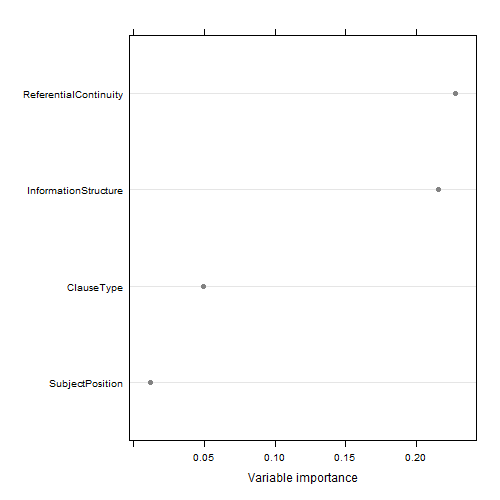
\includegraphics[width=3.125in,height=\textheight,keepaspectratio,alt={Variable importance plot showing four predictors ranked by their contribution to the model. ReferentialContinuity has the highest variable importance, followed by InformationStructure, ClauseType, and SubjectPosition.}]{1_Reproduction_Kocher/Analysis/Figures/varimp_native.png}

}

\caption{\label{fig-varimp-natives-kocher}Variable importance of the
native speaker of Spanish}

\end{figure}%

\newpage{}

I was likewise able to reproduce Figure 5 of Kocher
(\citeproc{ref-kocher_subject_2025}{2025}): 22, which shows the variable
importance of the random forest model predicting the target-likeness of
the L2 speakers (see Figure~\ref{fig-varimp-l2-kocher}). The reproduced
figure shows the same overall distribution as the original, with
\textsc{ReferentialContinuity} and \textsc{SubjectType} being the most
influential variables, followed by \textsc{ClauseType} and
\textsc{informationStructure}. \textsc{SubjectPosition} and the
(\textsc{Profociency)Score} contribute little to the model.

\begin{figure}

\centering{

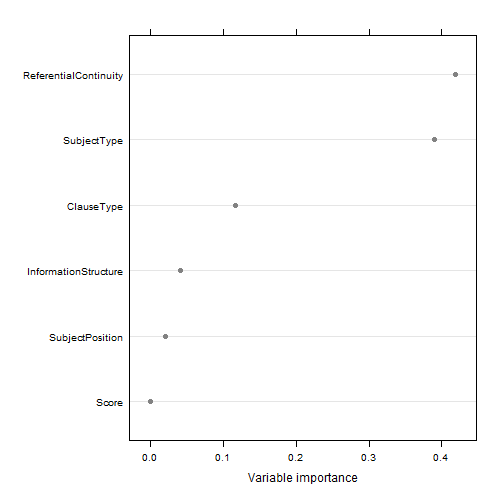
\includegraphics[width=3.125in,height=\textheight,keepaspectratio,alt={Variable importance plot showing the relative contribution of six predictors to the model. ReferentialContinuity is the most important variable, followed by SubjectType. ClauseType has moderate importance, while InformationStructure and SubjectPosition contribute less. The (Proficiency)Score has the lowest variable importance.}]{1_Reproduction_Kocher/Analysis/Figures/varimp_l2.png}

}

\caption{\label{fig-varimp-l2-kocher}Variable importance of the random
forest model of the \textsc{TargetLinkeness} of the L1 German speakers.}

\end{figure}%

{

\begin{longtable}[]{@{}lrr@{}}

\caption{\label{tbl-model-accuracy-l2}Reproduced confusion matrix for
the German L2 Spanish learner data. Rows indicate predicted subject
types, columns indicate actual subject types}

\tabularnewline

\toprule\noalign{}
& FALSE & TRUE \\
\midrule\noalign{}
\endhead
\bottomrule\noalign{}
\endlastfoot
FALSE & 701 & 0 \\
TRUE & 10 & 1624 \\

\end{longtable}

}

The results for the L2 speakers likewise closely match those reported by
Kocher. Whereas Kocher reports that the model has an ``extremely high
accuracy of prediction of 99\%'', the reproduced model achieves an
accuracy of 99.6\%. In total, only 10 observations are classified
incorrectly in the reproduced model, whereas this number is 11 in the
original analysis.

\subsubsection{Surrogate Decision Tree}\label{sec-1_surro}

First, I attempted to reproduce Kocher's original surrogate decision
tree (\citeproc{ref-kocher_subject_2025}{2025}: 24), but was not able to
reproduce it completely. For comparison, Kocher's original tree
Figure~\ref{fig-kocher-surro-original} is presented first.

\begin{figure}

\hfill\pandocbounded{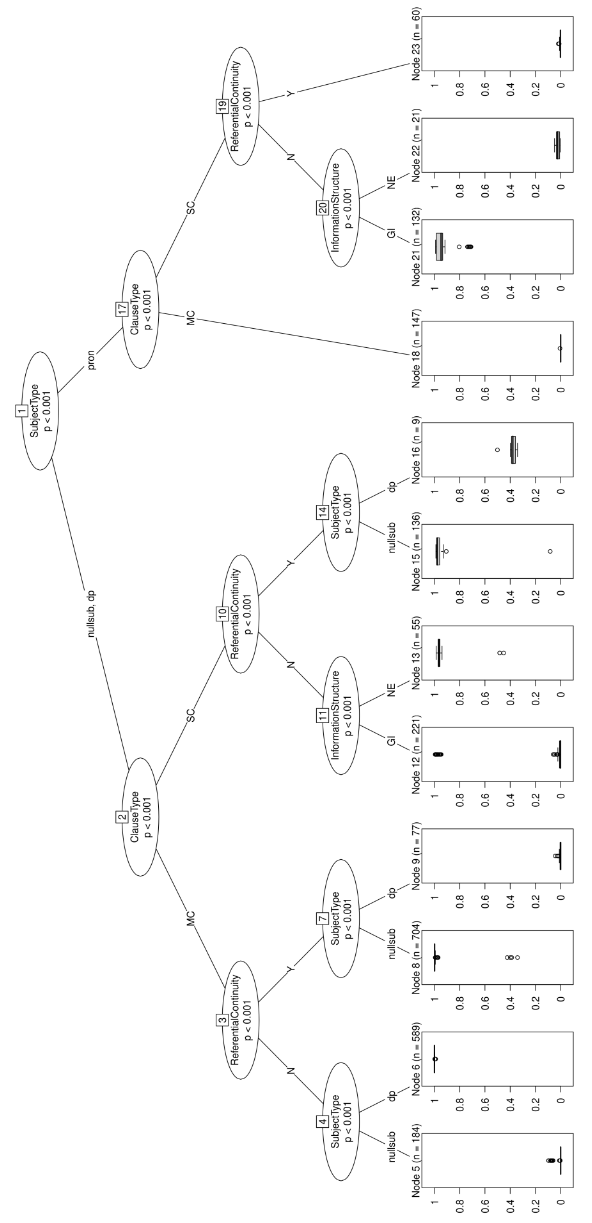
\includegraphics[keepaspectratio,alt={Kocher\textquotesingle s original decision-tree plot showing the recursive partitioning results for subject realisation. The tree first splits by SubjectType into pronoun versus nullsub, dp. The pronoun branch splits by ClauseType into MC and SC, followed by ReferentialContinuity and InformationStructure. The nullsub, dp branch similarly splits by ClauseType, then ReferentialContinuity, InformationStructure, and SubjectType. Terminal nodes display boxplots or distributions of the outcome values, with sample sizes ranging from 9 to 704. The split labels indicate statistical significance, with most splits marked p \textless{} 0.001.}]{1_Reproduction_Kocher/Analysis/Figures/Kocher_surrol2_landscape.png}}

\caption{\label{fig-kocher-surro-original}Kocher's original surrogate
tree of the random forest model of the TargetLikeness of the German L2
speakers with based on the original dataset.}

\end{figure}%

Figure~\ref{fig-kocher-surro-repro} shows the surrogate tree reproduced
using the same data.

\begin{figure}

\centering{

\pandocbounded{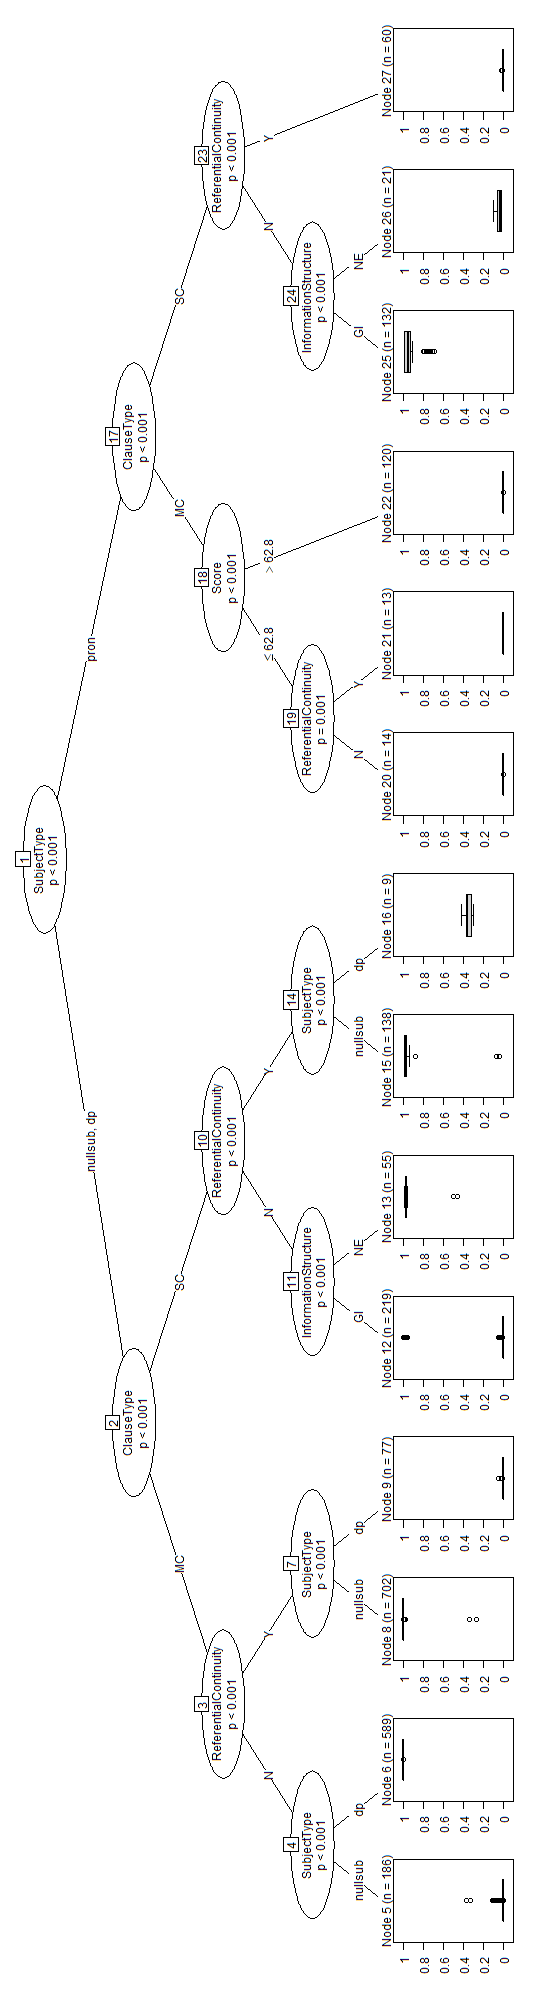
\includegraphics[keepaspectratio,alt={Reproduced decision tree showing subject realisation among L1 German L2 Spanish speakers. The first split is by SubjectType into pronoun and nullsub, dp. Both branches are then divided by ClauseType into main clauses (MC) and subordinate clauses (SC), followed by splits based on ReferentialContinuity, InformationStructure, SubjectType, and, for one pronoun branch, Score. The terminal nodes display distributions of the outcome variable with sample sizes ranging from 9 to 704. Most splits are statistically significant at p \textless{} 0.001. The tree illustrates that subject realisation varies according to subject form, clause type, referential (dis)continuity, information structure, and, in one branch, also the proficiency score.}]{1_Reproduction_Kocher/Analysis/Figures/surro_l2_landscape.png}}

}

\caption{\label{fig-kocher-surro-repro}Reproduced surrogate tree of the
random forest model of the \textsc{TargetLikeness} of the German L2
speakers with based on the original dataset.}

\end{figure}%

\newpage{}

Alike the original tree, the reproduced tree has a high R² of 0.945,
suggesting a good fit to the underlying random forest model. The only
difference between the two trees occurs at the first split on the
right-hand side, which represents the use of pronouns (node 17,
\textsc{ClauseType)}. In Kocher's tree, the left branch of this node
does not divide further and leads directly to terminal node 18. In the
reproduced tree, by contrast, MCs are further divided according to the
speakers' \textsc{(Proficency-)Score} and the
\textsc{ReferentialContinuity} of the subject (see node 20-22).

The boxplots at the terminal nodes represent the degree of reference- or
target-likeness, with 0 indicating a non-target-like and 1 a fully
target-like realisation. Consistent with Kocher's original tree, the MC
branch of the reproduced tree indicates that L1 German speakers do not
behave as predicted by the Spanish native speaker model when they use
pronouns, regardless of their \textsc{(Proficency-)Score.} In other
words, when L1 German learners use pronouns in these contexts, the
native speaker model predicts a different subject type, either a null
subject or a DP.

Among nodes 19-25, only node 20 shows a high degree of target-likeness.
This reproduces Kocher's finding that pronouns are particularly
difficult for L1 German learners to use in a target-like manner across
proficiency levels. Node 23 represents the target-like use of pronouns
in SC contexts when the subject is discontinuous but already given in
the discourse. Thus, pronouns tend to be used target-like in topic shift
contexts. As the remaining branches and boxplots closely correspond to
Kocher's findings, the use of DPs and null subjects is not discussed
further in the reproduction. Instead, these patterns are examined in the
following chapter in the context of the surrogate tree obtained in the
robustness check of Kocher's data (see
Section~\ref{sec-robustness-surro}).

\subsection{Robustness Check}\label{sec-RobustnessCheck}

\subsubsection{Robustness of Kocher's
annotation}\label{sec-RobustnessAnnotation}

The robustness check of Kocher's annotation was conducted on a sample of
three speakers comprising 118 clauses. The aim was to assess the
reliability and consistency of Kocher's annotation scheme. To this end,
inter-annotator agreement between Kocher's original annotation and my
re-annotation of the same clauses was calculated using Cohen's K,
implemented in the R package \{irr\} (version 0.84.1).

\begin{longtable}[]{@{}lrr@{}}
\caption{Inter-annotator agreement and Cohen's Kappa
values}\tabularnewline
\toprule\noalign{}
Variable & Agreement & CohensK \\
\midrule\noalign{}
\endfirsthead
\toprule\noalign{}
Variable & Agreement & CohensK \\
\midrule\noalign{}
\endhead
\bottomrule\noalign{}
\endlastfoot
SubjectType & 93.2 & 0.887 \\
ReferentialContinuity & 91.5 & 0.831 \\
ClauseType & 97.5 & 0.945 \\
InformationStructure & 95.8 & 0.739 \\
SubjectPosition & 100.0 & 1.000 \\
VerbConstruction & 93.2 & 0.803 \\
Verb & 97.5 & 0.974 \\
\end{longtable}

The resulting agreement values were interpreted according to the scale
proposed by Landis and Koch (\citeproc{ref-landiskoch1977}{1977}) (see
Appendix A, folder \texttt{1\_Reproduction\_Kocher}). The re-annotation
yielded high levels of agreement between Kocher's original annotation
and my annotation. Cohen's K ranged from 0.74 to 1, corresponding to
substantial to almost perfect agreement according to Landis and Koch
(\citeproc{ref-landiskoch1977}{1977}: 165). These results indicate that
the annotation scheme was applied consistently and suggest that the
manually annotated variables are sufficiently robust for the subsequent
analyses.

\subsubsection{Robustness Check by L1 German data
extension}\label{robustness-check-by-l1-german-data-extension}

The second part of the robustness check examines whether Kocher's
results remain stable when the same analysis is applied to an extended
L1 German dataset. The original scripts were therefore rerun using the
extended dataset, which contains additional L1 German speakers not
included in Kocher's original analysis.

\paragraph{Descriptive statistics and demographic
variables}\label{descriptive-statistics-and-demographic-variables-1}

\begin{longtable}[]{@{}
  >{\raggedright\arraybackslash}p{(\linewidth - 6\tabcolsep) * \real{0.4133}}
  >{\raggedright\arraybackslash}p{(\linewidth - 6\tabcolsep) * \real{0.1867}}
  >{\raggedright\arraybackslash}p{(\linewidth - 6\tabcolsep) * \real{0.1867}}
  >{\raggedright\arraybackslash}p{(\linewidth - 6\tabcolsep) * \real{0.1867}}@{}}
\caption{Proportion and frequency of subject type in the Spanish native
speaker and the L1 German learner of L2 Spanish
data.}\label{tbl-overview-frequencies}\tabularnewline
\toprule\noalign{}
\begin{minipage}[b]{\linewidth}\raggedright
\end{minipage} & \begin{minipage}[b]{\linewidth}\raggedright
dp
\end{minipage} & \begin{minipage}[b]{\linewidth}\raggedright
nullsub
\end{minipage} & \begin{minipage}[b]{\linewidth}\raggedright
pron
\end{minipage} \\
\midrule\noalign{}
\endfirsthead
\toprule\noalign{}
\begin{minipage}[b]{\linewidth}\raggedright
\end{minipage} & \begin{minipage}[b]{\linewidth}\raggedright
dp
\end{minipage} & \begin{minipage}[b]{\linewidth}\raggedright
nullsub
\end{minipage} & \begin{minipage}[b]{\linewidth}\raggedright
pron
\end{minipage} \\
\midrule\noalign{}
\endhead
\bottomrule\noalign{}
\endlastfoot
Spanish natives (L1), Kocher &
\begin{minipage}[t]{\linewidth}\raggedright
34.1\%\\
(178)\\
\strut
\end{minipage} & \begin{minipage}[t]{\linewidth}\raggedright
50\%\\
(261)\\
\strut
\end{minipage} & \begin{minipage}[t]{\linewidth}\raggedright
15.9\%\\
(83)\\
\strut
\end{minipage} \\
\begin{minipage}[t]{\linewidth}\raggedright
L1 German learners of\\
L2 Spanish (L2), Kocher\strut
\end{minipage} & \begin{minipage}[t]{\linewidth}\raggedright
37\%\\
(865)\\
\strut
\end{minipage} & \begin{minipage}[t]{\linewidth}\raggedright
47.5\%\\
(1110)\\
\strut
\end{minipage} & \begin{minipage}[t]{\linewidth}\raggedright
15.5\%\\
(360)\\
\strut
\end{minipage} \\
\begin{minipage}[t]{\linewidth}\raggedright
L1 German learners of\\
L2 Spanish (L2),\\
extended reproduction\strut
\end{minipage} & \begin{minipage}[t]{\linewidth}\raggedright
37.5\%\\
(1103)\\
\strut
\end{minipage} & \begin{minipage}[t]{\linewidth}\raggedright
47.2\%\\
(1389)\\
\strut
\end{minipage} & \begin{minipage}[t]{\linewidth}\raggedright
15.4\%\\
(453)\\
\strut
\end{minipage} \\
\end{longtable}

The overall distribution of DPs, null subjects, and pronouns in the
extended dataset is very similar to that of Kocher's original dataset
(see \citeproc{ref-kocher_subject_2025}{2025}: 16). DPs account for
37.5\% (1103), null subjects for 47.2\% (1389), and pronouns for 15.4\%
(453) of the extended L1 German data.

\begin{longtable}[]{@{}
  >{\raggedright\arraybackslash}p{(\linewidth - 12\tabcolsep) * \real{0.3068}}
  >{\centering\arraybackslash}p{(\linewidth - 12\tabcolsep) * \real{0.1023}}
  >{\centering\arraybackslash}p{(\linewidth - 12\tabcolsep) * \real{0.1023}}
  >{\centering\arraybackslash}p{(\linewidth - 12\tabcolsep) * \real{0.1136}}
  >{\centering\arraybackslash}p{(\linewidth - 12\tabcolsep) * \real{0.1136}}
  >{\centering\arraybackslash}p{(\linewidth - 12\tabcolsep) * \real{0.1023}}
  >{\centering\arraybackslash}p{(\linewidth - 12\tabcolsep) * \real{0.1023}}@{}}
\caption[Proportion and frequency of new versus given subjects by
subject type in the Spanish native speaker and the L1 German learner of
L2 Spanish data.]{Proportion and frequency of new versus given subjects
by subject type in the Spanish native speaker and the L1 German learner
of L2 Spanish data.\footnote{The missing percentages to 100\% are
  undisplayed values that are classified as NA in the extended dataset.}}\label{tbl-info-structure}\tabularnewline
\toprule\noalign{}
\begin{minipage}[b]{\linewidth}\raggedright
\end{minipage} & \begin{minipage}[b]{\linewidth}\centering
dp
\end{minipage} & \begin{minipage}[b]{\linewidth}\centering
dp
\end{minipage} & \begin{minipage}[b]{\linewidth}\centering
nullsub
\end{minipage} & \begin{minipage}[b]{\linewidth}\centering
nullsub
\end{minipage} & \begin{minipage}[b]{\linewidth}\centering
pron
\end{minipage} & \begin{minipage}[b]{\linewidth}\centering
pron
\end{minipage} \\
\midrule\noalign{}
\endfirsthead
\toprule\noalign{}
\begin{minipage}[b]{\linewidth}\raggedright
\end{minipage} & \begin{minipage}[b]{\linewidth}\centering
dp
\end{minipage} & \begin{minipage}[b]{\linewidth}\centering
dp
\end{minipage} & \begin{minipage}[b]{\linewidth}\centering
nullsub
\end{minipage} & \begin{minipage}[b]{\linewidth}\centering
nullsub
\end{minipage} & \begin{minipage}[b]{\linewidth}\centering
pron
\end{minipage} & \begin{minipage}[b]{\linewidth}\centering
pron
\end{minipage} \\
\midrule\noalign{}
\endhead
\bottomrule\noalign{}
\endlastfoot
& Given & New & Given & New & Given & New \\
L1, Kocher & \begin{minipage}[t]{\linewidth}\centering
59.5\%\\
(106)\\
\strut
\end{minipage} & \begin{minipage}[t]{\linewidth}\centering
40.5\%\\
(72)\\
\strut
\end{minipage} & \begin{minipage}[t]{\linewidth}\centering
96.1\%\\
(248)\\
\strut
\end{minipage} & \begin{minipage}[t]{\linewidth}\centering
3.9\%\\
(10)\\
\strut
\end{minipage} & \begin{minipage}[t]{\linewidth}\centering
84.1\%\\
(69)-\\
\strut
\end{minipage} & \begin{minipage}[t]{\linewidth}\centering
15.9\%\\
(13)\\
\strut
\end{minipage} \\
L2, Kocher & \begin{minipage}[t]{\linewidth}\centering
71.1\%\\
(615)\\
\strut
\end{minipage} & \begin{minipage}[t]{\linewidth}\centering
28.9\%\\
(250)\\
\strut
\end{minipage} & \begin{minipage}[t]{\linewidth}\centering
98.5\%\\
(1084)\\
\strut
\end{minipage} & \begin{minipage}[t]{\linewidth}\centering
1.5\%\\
(16)\\
\strut
\end{minipage} & \begin{minipage}[t]{\linewidth}\centering
89.4\%\\
(322)\\
\strut
\end{minipage} & \begin{minipage}[t]{\linewidth}\centering
10.6\%\\
(38)\\
\strut
\end{minipage} \\
L2 extended Reproduction & \begin{minipage}[t]{\linewidth}\centering
72.3\%\\
(798)\\
\strut
\end{minipage} & \begin{minipage}[t]{\linewidth}\centering
27.6\%\\
(304)\\
\strut
\end{minipage} & \begin{minipage}[t]{\linewidth}\centering
97.2\%\\
(1350)\\
\strut
\end{minipage} & \begin{minipage}[t]{\linewidth}\centering
1.4\%\\
(20)\\
\strut
\end{minipage} & \begin{minipage}[t]{\linewidth}\centering
89.2\%\\
(404)\\
\strut
\end{minipage} & \begin{minipage}[t]{\linewidth}\centering
9.1\%\\
(41)\\
\strut
\end{minipage} \\
\end{longtable}

The distribution of new and given subjects by subject type likewise
remains similar to that reported by Kocher
(\citeproc{ref-kocher_subject_2025}{2025}: 16). As in Kocher's dataset,
the differences between new and given referents are particularly
pronounced in the L2 data. In the extended dataset, given referents
account for 72.3\% of DPs, 97.2\% of null subjects, and 89.2\% of
pronouns, while new referents account for 27.6\%, 1.4\%, and 9.1\%,
respectively. The association between \textsc{SubjectType} and
\textsc{InformationStructure} is statistically significant (X² = 386.03,
\emph{p} \textless{} 0.001).

\begin{longtable}[]{@{}
  >{\raggedright\arraybackslash}p{(\linewidth - 12\tabcolsep) * \real{0.2269}}
  >{\centering\arraybackslash}p{(\linewidth - 12\tabcolsep) * \real{0.1092}}
  >{\centering\arraybackslash}p{(\linewidth - 12\tabcolsep) * \real{0.1345}}
  >{\centering\arraybackslash}p{(\linewidth - 12\tabcolsep) * \real{0.1092}}
  >{\centering\arraybackslash}p{(\linewidth - 12\tabcolsep) * \real{0.1345}}
  >{\centering\arraybackslash}p{(\linewidth - 12\tabcolsep) * \real{0.1092}}
  >{\centering\arraybackslash}p{(\linewidth - 12\tabcolsep) * \real{0.1345}}@{}}
\caption[Proportion and frequency of (dis-)continuous referents by type
in the Spanish native speaker and the L1 German learner of L2 Spanish
data.]{Proportion and frequency of (dis-)continuous referents by type in
the Spanish native speaker and the L1 German learner of L2 Spanish
data.\footnote{The missing percentages to 100\% are undisplayed values
  that are classified as NA in the extended dataset.}}\label{tbl-referential-continuity}\tabularnewline
\toprule\noalign{}
\begin{minipage}[b]{\linewidth}\raggedright
\end{minipage} & \begin{minipage}[b]{\linewidth}\centering
dp
\end{minipage} & \begin{minipage}[b]{\linewidth}\centering
dp
\end{minipage} & \begin{minipage}[b]{\linewidth}\centering
nullsub
\end{minipage} & \begin{minipage}[b]{\linewidth}\centering
nullsub
\end{minipage} & \begin{minipage}[b]{\linewidth}\centering
pron
\end{minipage} & \begin{minipage}[b]{\linewidth}\centering
pron
\end{minipage} \\
\midrule\noalign{}
\endfirsthead
\toprule\noalign{}
\begin{minipage}[b]{\linewidth}\raggedright
\end{minipage} & \begin{minipage}[b]{\linewidth}\centering
dp
\end{minipage} & \begin{minipage}[b]{\linewidth}\centering
dp
\end{minipage} & \begin{minipage}[b]{\linewidth}\centering
nullsub
\end{minipage} & \begin{minipage}[b]{\linewidth}\centering
nullsub
\end{minipage} & \begin{minipage}[b]{\linewidth}\centering
pron
\end{minipage} & \begin{minipage}[b]{\linewidth}\centering
pron
\end{minipage} \\
\midrule\noalign{}
\endhead
\bottomrule\noalign{}
\endlastfoot
& Continuous & Discontinuous & Continuous & Discontinuous & Continuous &
Discontinuous \\
L1, Kocher & \begin{minipage}[t]{\linewidth}\centering
9\%\\
(16)\\
\strut
\end{minipage} & \begin{minipage}[t]{\linewidth}\centering
91\%\\
(162)\\
\strut
\end{minipage} & \begin{minipage}[t]{\linewidth}\centering
61.5\%\\
(158)\\
\strut
\end{minipage} & \begin{minipage}[t]{\linewidth}\centering
38.5\%\\
(99)\\
\strut
\end{minipage} & \begin{minipage}[t]{\linewidth}\centering
29\%\\
(24)\\
\strut
\end{minipage} & \begin{minipage}[t]{\linewidth}\centering
71\%\\
(59)\\
\strut
\end{minipage} \\
L2, Kocher & \begin{minipage}[t]{\linewidth}\centering
10\%\\
(86)\\
\strut
\end{minipage} & \begin{minipage}[t]{\linewidth}\centering
90\%\\
(779)\\
\strut
\end{minipage} & \begin{minipage}[t]{\linewidth}\centering
76\%\\
(835)\\
\strut
\end{minipage} & \begin{minipage}[t]{\linewidth}\centering
24\%\\
(265)\\
\strut
\end{minipage} & \begin{minipage}[t]{\linewidth}\centering
32\%\\
(115)\\
\strut
\end{minipage} & \begin{minipage}[t]{\linewidth}\centering
68\%\\
(245)\\
\strut
\end{minipage} \\
L2 extended Reproduction & \begin{minipage}[t]{\linewidth}\centering
11\%\\
(121)\\
\strut
\end{minipage} & \begin{minipage}[t]{\linewidth}\centering
89\%\\
(982)\\
\strut
\end{minipage} & \begin{minipage}[t]{\linewidth}\centering
75\%\\
(1042)\\
\strut
\end{minipage} & \begin{minipage}[t]{\linewidth}\centering
24.3\%\\
(337)\\
\strut
\end{minipage} & \begin{minipage}[t]{\linewidth}\centering
33.6\%\\
(152)\\
\strut
\end{minipage} & \begin{minipage}[t]{\linewidth}\centering
66.4\%\\
(301)\\
\strut
\end{minipage} \\
\end{longtable}

The distribution of continuous and discontinuous referents also remains
similar to Kocher's results (\citeproc{ref-kocher_subject_2025}{2025}:
16). In the extended dataset, null subjects are predominantly used with
continuous referents, whereas DPs and pronouns occur more frequently
with discontinuous referents. The association between
\textsc{SubjectType} and \textsc{ReferentialContinuity} is statistically
significant (X² = 1061.3, \emph{p} \textless{} 0.001).

\begin{longtable}[]{@{}
  >{\raggedright\arraybackslash}p{(\linewidth - 12\tabcolsep) * \real{0.3068}}
  >{\centering\arraybackslash}p{(\linewidth - 12\tabcolsep) * \real{0.1023}}
  >{\centering\arraybackslash}p{(\linewidth - 12\tabcolsep) * \real{0.1023}}
  >{\centering\arraybackslash}p{(\linewidth - 12\tabcolsep) * \real{0.1136}}
  >{\centering\arraybackslash}p{(\linewidth - 12\tabcolsep) * \real{0.1136}}
  >{\centering\arraybackslash}p{(\linewidth - 12\tabcolsep) * \real{0.1023}}
  >{\centering\arraybackslash}p{(\linewidth - 12\tabcolsep) * \real{0.1023}}@{}}
\caption{Proportion and frequency of MCs versus SCs by type in the
Spanish native speaker and the L1 German learner of L2 Spanish
data.}\label{tbl-clause-type}\tabularnewline
\toprule\noalign{}
\begin{minipage}[b]{\linewidth}\raggedright
\end{minipage} & \begin{minipage}[b]{\linewidth}\centering
dp
\end{minipage} & \begin{minipage}[b]{\linewidth}\centering
dp
\end{minipage} & \begin{minipage}[b]{\linewidth}\centering
nullsub
\end{minipage} & \begin{minipage}[b]{\linewidth}\centering
nullsub
\end{minipage} & \begin{minipage}[b]{\linewidth}\centering
pron
\end{minipage} & \begin{minipage}[b]{\linewidth}\centering
pron
\end{minipage} \\
\midrule\noalign{}
\endfirsthead
\toprule\noalign{}
\begin{minipage}[b]{\linewidth}\raggedright
\end{minipage} & \begin{minipage}[b]{\linewidth}\centering
dp
\end{minipage} & \begin{minipage}[b]{\linewidth}\centering
dp
\end{minipage} & \begin{minipage}[b]{\linewidth}\centering
nullsub
\end{minipage} & \begin{minipage}[b]{\linewidth}\centering
nullsub
\end{minipage} & \begin{minipage}[b]{\linewidth}\centering
pron
\end{minipage} & \begin{minipage}[b]{\linewidth}\centering
pron
\end{minipage} \\
\midrule\noalign{}
\endhead
\bottomrule\noalign{}
\endlastfoot
& MC & SC & MC & SC & MC & SC \\
L1, Kocher & \begin{minipage}[t]{\linewidth}\centering
75.8\%\\
(135)\\
\strut
\end{minipage} & \begin{minipage}[t]{\linewidth}\centering
24.2\%\\
(43)\\
\strut
\end{minipage} & \begin{minipage}[t]{\linewidth}\centering
72\%\\
(188)\\
\strut
\end{minipage} & \begin{minipage}[t]{\linewidth}\centering
28\%\\
(73)\\
\strut
\end{minipage} & \begin{minipage}[t]{\linewidth}\centering
26.5\%\\
(22)\\
\strut
\end{minipage} & \begin{minipage}[t]{\linewidth}\centering
73.5\%\\
(61)\\
\strut
\end{minipage} \\
L2, Kocher & \begin{minipage}[t]{\linewidth}\centering
77\%\\
(666)\\
\strut
\end{minipage} & \begin{minipage}[t]{\linewidth}\centering
23\%\\
(199)\\
\strut
\end{minipage} & \begin{minipage}[t]{\linewidth}\centering
80\%\\
(888)\\
\strut
\end{minipage} & \begin{minipage}[t]{\linewidth}\centering
20\%\\
(222)\\
\strut
\end{minipage} & \begin{minipage}[t]{\linewidth}\centering
40.8\%\\
(147)\\
\strut
\end{minipage} & \begin{minipage}[t]{\linewidth}\centering
59.2\%\\
(213)\\
\strut
\end{minipage} \\
L2 extended Reproduction & \begin{minipage}[t]{\linewidth}\centering
76.8\%\\
(847)\\
\strut
\end{minipage} & \begin{minipage}[t]{\linewidth}\centering
23.2\%\\
(256)\\
\strut
\end{minipage} & \begin{minipage}[t]{\linewidth}\centering
79.9\%\\
(1110)\\
\strut
\end{minipage} & \begin{minipage}[t]{\linewidth}\centering
20.1\%\\
(279)\\
\strut
\end{minipage} & \begin{minipage}[t]{\linewidth}\centering
42.8\%\\
(194)\\
\strut
\end{minipage} & \begin{minipage}[t]{\linewidth}\centering
57.2\%\\
(259)\\
\strut
\end{minipage} \\
\end{longtable}

The distribution of MCs and SCs likewise shows little change compared
with Kocher's dataset. DPs and null subjects occur more frequently in
MCs, whereas pronouns are more frequent in SCs in both the original and
extended datasets (\citeproc{ref-kocher_subject_2025}{2025}: 17). The
association between \textsc{SubjectType} and \textsc{ClauseType} is
statistically significant (X² = 251.21, \emph{p} \textless{} 0.001).

\begin{longtable}[]{@{}
  >{\raggedright\arraybackslash}p{(\linewidth - 8\tabcolsep) * \real{0.3375}}
  >{\centering\arraybackslash}p{(\linewidth - 8\tabcolsep) * \real{0.1500}}
  >{\centering\arraybackslash}p{(\linewidth - 8\tabcolsep) * \real{0.1625}}
  >{\centering\arraybackslash}p{(\linewidth - 8\tabcolsep) * \real{0.1500}}
  >{\centering\arraybackslash}p{(\linewidth - 8\tabcolsep) * \real{0.1625}}@{}}
\caption{Proportion and frequency of pre- and postverbal subjects by
type in the Spanish native speaker and the L1 German learner of L2
Spanish data.}\label{tbl-subject-position}\tabularnewline
\toprule\noalign{}
\begin{minipage}[b]{\linewidth}\raggedright
\end{minipage} & \begin{minipage}[b]{\linewidth}\centering
dp
\end{minipage} & \begin{minipage}[b]{\linewidth}\centering
dp
\end{minipage} & \begin{minipage}[b]{\linewidth}\centering
pron
\end{minipage} & \begin{minipage}[b]{\linewidth}\centering
pron
\end{minipage} \\
\midrule\noalign{}
\endfirsthead
\toprule\noalign{}
\begin{minipage}[b]{\linewidth}\raggedright
\end{minipage} & \begin{minipage}[b]{\linewidth}\centering
dp
\end{minipage} & \begin{minipage}[b]{\linewidth}\centering
dp
\end{minipage} & \begin{minipage}[b]{\linewidth}\centering
pron
\end{minipage} & \begin{minipage}[b]{\linewidth}\centering
pron
\end{minipage} \\
\midrule\noalign{}
\endhead
\bottomrule\noalign{}
\endlastfoot
& Preverbal & Postverbal & Preverbal & Postverbal \\
L1, Kocher & \begin{minipage}[t]{\linewidth}\centering
77.5\%\\
(138)\\
\strut
\end{minipage} & \begin{minipage}[t]{\linewidth}\centering
22.5\%\\
(40)\\
\strut
\end{minipage} & \begin{minipage}[t]{\linewidth}\centering
95\%\\
(77)\\
\strut
\end{minipage} & \begin{minipage}[t]{\linewidth}\centering
5\%\\
(4)\\
\strut
\end{minipage} \\
L2, Kocher & \begin{minipage}[t]{\linewidth}\centering
86\%\\
(737)\\
\strut
\end{minipage} & \begin{minipage}[t]{\linewidth}\centering
14\%\\
(119)\\
\strut
\end{minipage} & \begin{minipage}[t]{\linewidth}\centering
96.1\%\\
(346)\\
\strut
\end{minipage} & \begin{minipage}[t]{\linewidth}\centering
3.9\%\\
(14)\\
\strut
\end{minipage} \\
L2 extended Reproduction & \begin{minipage}[t]{\linewidth}\centering
86.3\%\\
(934)\\
\strut
\end{minipage} & \begin{minipage}[t]{\linewidth}\centering
13.7\%\\
(148)\\
\strut
\end{minipage} & \begin{minipage}[t]{\linewidth}\centering
96.1\%\\
(423)\\
\strut
\end{minipage} & \begin{minipage}[t]{\linewidth}\centering
3.9\%\\
(17)\\
\strut
\end{minipage} \\
\end{longtable}

The distribution of preverbal and postverbal subjects is also highly
similar to Kocher's dataset. As preverbal position is the unmarked
subject position with most Spanish verbs, both subject types are
expected to occur predominantly in this position (see
\citeproc{ref-kocher_subject_2025}{2025}: 17). In the extended dataset,
86.3\% of DPs and 96.1\% of pronouns occur preverbally. As in the native
speaker data, pronouns are used almost exclusively in preverbal
position, whereas DPs occur slightly more frequently postverbally. The
association between \textsc{SubjectType} and \textsc{SubjectPosition} is
statistically significant (X² = 30.167, \emph{p} \textless{} 0.001). As
in Kocher's dataset, most of the postverbal subjects in the extended L2
data occur with presentative \emph{ser} and unaccusative verbs such as
\emph{venir, aparecer, pasar, caer,} and \emph{estar} (compare
\citeproc{ref-kocher_subject_2025}{Kocher, 2025}: 18).

\begin{longtable}[]{@{}
  >{\raggedright\arraybackslash}p{(\linewidth - 18\tabcolsep) * \real{0.1000}}
  >{\raggedright\arraybackslash}p{(\linewidth - 18\tabcolsep) * \real{0.1000}}
  >{\raggedright\arraybackslash}p{(\linewidth - 18\tabcolsep) * \real{0.1000}}
  >{\raggedright\arraybackslash}p{(\linewidth - 18\tabcolsep) * \real{0.1000}}
  >{\raggedright\arraybackslash}p{(\linewidth - 18\tabcolsep) * \real{0.1000}}
  >{\raggedright\arraybackslash}p{(\linewidth - 18\tabcolsep) * \real{0.1000}}
  >{\raggedright\arraybackslash}p{(\linewidth - 18\tabcolsep) * \real{0.1000}}
  >{\raggedright\arraybackslash}p{(\linewidth - 18\tabcolsep) * \real{0.1000}}
  >{\raggedright\arraybackslash}p{(\linewidth - 18\tabcolsep) * \real{0.1000}}
  >{\raggedright\arraybackslash}p{(\linewidth - 18\tabcolsep) * \real{0.1000}}@{}}
\caption{Proportion and frequency of masculine and feminine subjects by
type in the Spanish native speaker and the L1 German learner of L2
Spanish data.}\label{tbl-genus}\tabularnewline
\toprule\noalign{}
\begin{minipage}[b]{\linewidth}\raggedright
\end{minipage} & \begin{minipage}[b]{\linewidth}\raggedright
masc
\end{minipage} & \begin{minipage}[b]{\linewidth}\raggedright
masc
\end{minipage} & \begin{minipage}[b]{\linewidth}\raggedright
masc
\end{minipage} & \begin{minipage}[b]{\linewidth}\raggedright
fem
\end{minipage} & \begin{minipage}[b]{\linewidth}\raggedright
fem
\end{minipage} & \begin{minipage}[b]{\linewidth}\raggedright
fem
\end{minipage} & \begin{minipage}[b]{\linewidth}\raggedright
unknown
\end{minipage} & \begin{minipage}[b]{\linewidth}\raggedright
unknown
\end{minipage} & \begin{minipage}[b]{\linewidth}\raggedright
unknown
\end{minipage} \\
\midrule\noalign{}
\endfirsthead
\toprule\noalign{}
\begin{minipage}[b]{\linewidth}\raggedright
\end{minipage} & \begin{minipage}[b]{\linewidth}\raggedright
masc
\end{minipage} & \begin{minipage}[b]{\linewidth}\raggedright
masc
\end{minipage} & \begin{minipage}[b]{\linewidth}\raggedright
masc
\end{minipage} & \begin{minipage}[b]{\linewidth}\raggedright
fem
\end{minipage} & \begin{minipage}[b]{\linewidth}\raggedright
fem
\end{minipage} & \begin{minipage}[b]{\linewidth}\raggedright
fem
\end{minipage} & \begin{minipage}[b]{\linewidth}\raggedright
unknown
\end{minipage} & \begin{minipage}[b]{\linewidth}\raggedright
unknown
\end{minipage} & \begin{minipage}[b]{\linewidth}\raggedright
unknown
\end{minipage} \\
\midrule\noalign{}
\endhead
\bottomrule\noalign{}
\endlastfoot
& dp & nullsub & pron & dp & nullsub & pron & dp & nullsub & pron \\
L1 & 31.8 (127) & 55.9\% (223) & 12.3\% (49) & 48.5\% (48) & 27.3\     (27)
& 24.2\% (24) & 10\% (2) & 40\% (8) & 50\% (10) \\
L2 extended dataset & 36.3\% (822) & 51.5\% (1167) & 12.3\% (278) & 46\%
(274) & 31\% (185) & 23\% (137) & 5.1\% (3) & 30.5\% (18) & 64.4\%
(38) \\
\end{longtable}

The annotation of \textsc{SubjectGenus} makes it possible to examine the
distribution of masculine and feminine referents across subject types.
Null subjects can refer to either masculine or feminine referents, so
grammatical gender cannot be inferred from the formal realisation of the
subject alone. The predominance of masculine referents in the data can
be attributed to their unequal distribution in the corpus. The film
sequence contains substantially more predominantly human masculine
subjects (\emph{N} = 2267), including \emph{Chaplin, el bebé, el otro
bebé, el viejo, el policía, el señor,} and \emph{el protagonista}, than
feminine subjects (\emph{N} = 596), such as \emph{la mujer, la policía,
la persona, la madre,} and \emph{la carta}.

Within this overall distribution, masculine and feminine referents also
differ in their proportional realisation across subject types. In both
the L1 and L2 datasets, masculine referents are most frequently realised
as null subjects, whereas feminine referents are most frequently
realised as DPs. Feminine referents are also proportionally more often
realised as pronouns than masculine referents. Subjects whose referents
cannot be identified are most frequently realised as pronouns, but also
occur as null subjects.

The association between \textsc{SubjectGenus} and \textsc{SubjectType}
is statistically significant in both the Spanish native speaker data (X²
= 45.511, \emph{p} \textless{} 0.001) and the L2 data (X² = 202.16,
\emph{p} \textless{} 0.001). Thus, the results do not support Da Cunha's
finding that masculine referents are generally realised more diversely
than feminine referents (\citeproc{ref-dacunha2024}{2024}: iii).
However, the data support the prediction that masculine subjects are
more frequently realised as DPs than as pronouns, whereas the
distribution of DPs and pronouns is more balanced among feminine
referents. In both the L1 and L2 datasets, however, masculine referents
predominantly occur as null subjects (86.4\% and 85.2\%\footnote{When
  grouped not by SubjectGenus but by SubjectType.}, respectively).

\begin{longtable}[]{@{}
  >{\raggedright\arraybackslash}p{(\linewidth - 12\tabcolsep) * \real{0.2619}}
  >{\centering\arraybackslash}p{(\linewidth - 12\tabcolsep) * \real{0.1071}}
  >{\centering\arraybackslash}p{(\linewidth - 12\tabcolsep) * \real{0.1071}}
  >{\centering\arraybackslash}p{(\linewidth - 12\tabcolsep) * \real{0.1190}}
  >{\centering\arraybackslash}p{(\linewidth - 12\tabcolsep) * \real{0.1190}}
  >{\centering\arraybackslash}p{(\linewidth - 12\tabcolsep) * \real{0.1071}}
  >{\centering\arraybackslash}p{(\linewidth - 12\tabcolsep) * \real{0.1190}}@{}}
\caption{Proportion and frequency of masculine and feminine subjects by
the speaker's gender in the Spanish native speaker and the L1 German
learner of L2 Spanish data.}\label{tbl-gender-genus}\tabularnewline
\toprule\noalign{}
\begin{minipage}[b]{\linewidth}\raggedright
\end{minipage} & \begin{minipage}[b]{\linewidth}\centering
Male
\end{minipage} & \begin{minipage}[b]{\linewidth}\centering
Male
\end{minipage} & \begin{minipage}[b]{\linewidth}\centering
Male
\end{minipage} & \begin{minipage}[b]{\linewidth}\centering
Female
\end{minipage} & \begin{minipage}[b]{\linewidth}\centering
Female
\end{minipage} & \begin{minipage}[b]{\linewidth}\centering
Female
\end{minipage} \\
\midrule\noalign{}
\endfirsthead
\toprule\noalign{}
\begin{minipage}[b]{\linewidth}\raggedright
\end{minipage} & \begin{minipage}[b]{\linewidth}\centering
Male
\end{minipage} & \begin{minipage}[b]{\linewidth}\centering
Male
\end{minipage} & \begin{minipage}[b]{\linewidth}\centering
Male
\end{minipage} & \begin{minipage}[b]{\linewidth}\centering
Female
\end{minipage} & \begin{minipage}[b]{\linewidth}\centering
Female
\end{minipage} & \begin{minipage}[b]{\linewidth}\centering
Female
\end{minipage} \\
\midrule\noalign{}
\endhead
\bottomrule\noalign{}
\endlastfoot
& masc & fem & unknown & masc & fem & unknown \\
L1 & \begin{minipage}[t]{\linewidth}\centering
77\%\\
(154)\\
\strut
\end{minipage} & \begin{minipage}[t]{\linewidth}\centering
19.5\%\\
(39)\\
\strut
\end{minipage} & \begin{minipage}[t]{\linewidth}\centering
3.5\%\\
(7)\\
\strut
\end{minipage} & \begin{minipage}[t]{\linewidth}\centering
77\%\\
(245)\\
\strut
\end{minipage} & \begin{minipage}[t]{\linewidth}\centering
18.9\%\\
(60)\\
\strut
\end{minipage} & \begin{minipage}[t]{\linewidth}\centering
4.1\%\\
(13)\\
\strut
\end{minipage} \\
L2 extended dataset & \begin{minipage}[t]{\linewidth}\centering
80\%\\
(411)\\
\strut
\end{minipage} & \begin{minipage}[t]{\linewidth}\centering
19.3\%\\
(99)\\
\strut
\end{minipage} & \begin{minipage}[t]{\linewidth}\centering
0.8\%\\
(4)\\
\strut
\end{minipage} & \begin{minipage}[t]{\linewidth}\centering
77.1\%\\
(1856)\\
\strut
\end{minipage} & \begin{minipage}[t]{\linewidth}\centering
20.6\%\\
(497)\\
\strut
\end{minipage} & \begin{minipage}[t]{\linewidth}\centering
2.3\%\\
(55)\\
\strut
\end{minipage} \\
\end{longtable}

The distribution of subject genus by speaker gender shows a similar
pattern to that reported by Da Cunha for male and female speakers
(\citeproc{ref-dacunha2024}{2024}: 189). In the present native speaker
and L1 German data, both male and female speakers predominantly produce
masculine subjects. Thus, unlike Da Cunha's study, the present data do
not show a ``biais nul'' among female speakers
(\citeproc{ref-dacunha2024}{2024}: 194). However, the differences
between male and female speakers are not statistically significant in
either the native speaker data (X² = 0.13566, \emph{p} \textgreater{}
0.05) or the L2 German data (X² = 5.6061, \emph{p} \textgreater{} 0.05).

As the native speaker data remain unchanged in the robustness check, it
is not necessary to repeat the reproduction of the native speaker model
accuracy and variable importance. The following section therefore
focuses on the extended L1 German data, beginning with the distribution
of clauses across the three proficiency groups.

Figure~\ref{fig-scores-german-extended} shows that the proficiency
distribution among the L2 speakers remains skewed towards advanced
learners. Only one speaker has a score below 33, while 14 speakers have
scores between 33 and 66; the remaining 85 speakers have scores of 66 or
higher (see also \citeproc{ref-kocher_subject_2025}{Kocher, 2025}: 18).
As in the original dataset, there is no significant difference in the
distribution of subject types depending on whether speakers have
knowledge of an additional null subject language (X² = 1.5, \emph{p}
\textgreater{} 0.05).

\begin{figure}

\centering{

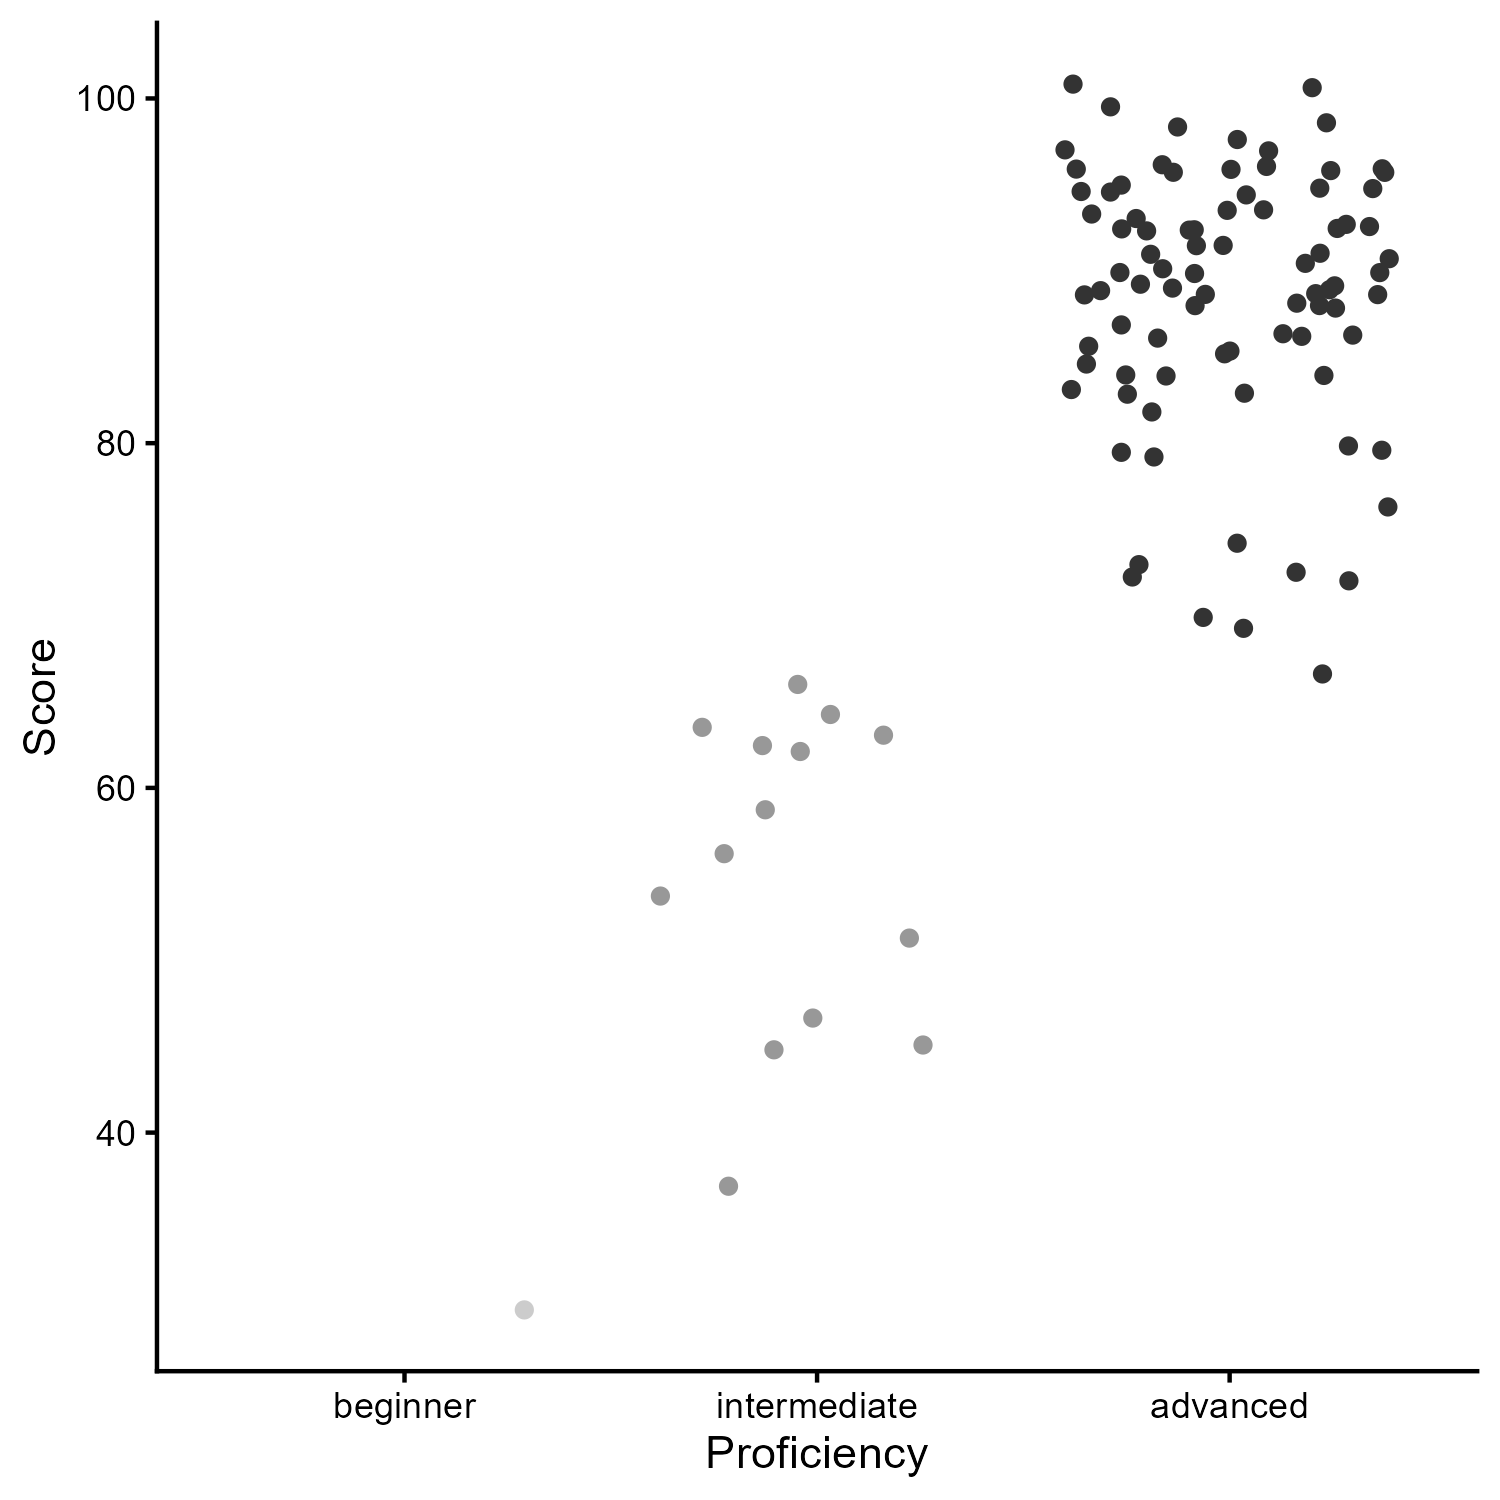
\includegraphics[width=2.60417in,height=\textheight,keepaspectratio]{2_Robustness_Check/Figures/Scores.png}

}

\caption{\label{fig-scores-german-extended}Placement score of each
speaker in the extended L2 German dataset, light gray: beginners
(\textless33), gray: intermediate (33\textgreater66), black: advanced
(\textgreater66).}

\end{figure}%

\newpage{}

\paragraph{Variable importance and Model accuracy of the extended German
L2 learners of Spanish
dataset}\label{variable-importance-and-model-accuracy-of-the-extended-german-l2-learners-of-spanish-dataset}

As neither the native speaker data nor the native speaker model was
changed in the robustness check, the native speaker variable importance
plot and model accuracy remain unchanged. I therefore report only the
variable importance of the final L1 German model. Despite the larger
dataset, the distribution of variable importance is very similar to that
obtained in the reproduction based on Kocher's original data.

\begin{figure}

\centering{

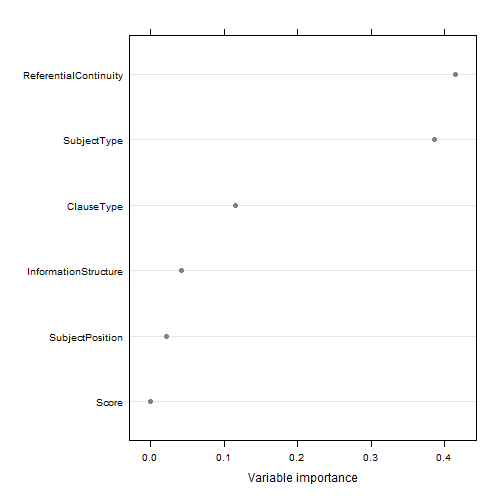
\includegraphics[width=3.125in,height=\textheight,keepaspectratio,alt={Dot plot showing the variable importance of six predictors in an L2 Spanish subject-realisation model. ReferentialContinuity has the highest variable importance, followed by SubjectType. As for less important variables follow ClauseType, InformationStructure, SubjectPosition, and Score. The x-axis represents variable importance.}]{2_Robustness_Check/Figures/varimp_l2.png}

}

\caption{\label{fig-varimp-germanl2-extended}Variable importance of the
random forest model of the \textsc{TargetLinkeness} of the L2 speakers.}

\end{figure}%

\newpage{}

The confusion matrix for the extended L2 German dataset is presented
below. As in the original analysis, the columns represent the observed
subject types in the L2 data, whereas the rows represent the subject
types predicted by the L1 model (see
\citeproc{ref-kocher_subject_2025}{Kocher, 2025}: 21).

\begin{longtable}[]{@{}lrr@{}}
\caption{Reproduced confusion matrix for the extended German L2 Spanish
learner data. Rows indicate predicted subject types, columns indicate
actual subject types}\tabularnewline
\toprule\noalign{}
& FALSE & TRUE \\
\midrule\noalign{}
\endfirsthead
\toprule\noalign{}
& FALSE & TRUE \\
\midrule\noalign{}
\endhead
\bottomrule\noalign{}
\endlastfoot
FALSE & 710 & 0 \\
TRUE & 14 & 1660 \\
\end{longtable}

The extended L2 German model achieves an accuracy of 99.4\%, which is
the same as the accuracy obtained with Kocher's original L2 dataset. In
total, 14 observations are classified incorrectly.

\paragraph{Surrogate Decision Tree}\label{sec-robustness-surro}

Figure~\ref{fig-robustness-surro} displays the surrogate tree of the
random forest model of the target-likeness of the L1 German learners of
Spanish based on the extended dataset. The surrogate model has an R² of
0.945, which, as in the original analysis, indicates a good fit to the
underlying random forest model.

\begin{figure}

\centering{

\pandocbounded{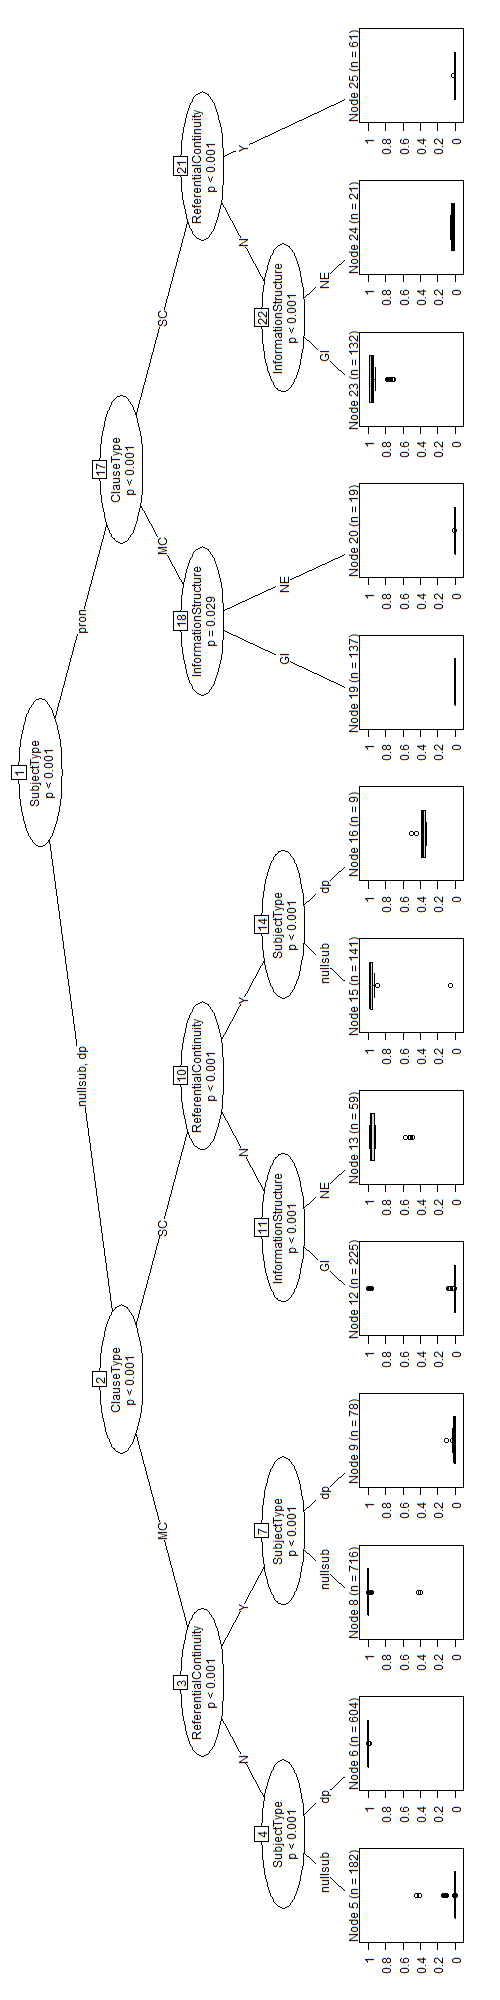
\includegraphics[keepaspectratio,alt={A recursive partitioning tree showing subject realisation in the Spanish native speaker data. The first split is by SubjectType, separating pronoun from nullsub, dp. Both branches are then divided by ClauseType into main clauses (MC) and subordinate clauses (SC). Subsequent splits involve ReferentialContinuity, InformationStructure, and, in several branches, SubjectType. The terminal nodes display distributions of the outcome variable, with sample sizes ranging from 9 to 604.}]{2_Robustness_Check/Figures/surro_landscape.png}}

}

\caption{\label{fig-robustness-surro}Reproduced surrogate tree of the
random forest model of the TargetLikeness of the L1 German learners of
Spanish based on the extended dataset.}

\end{figure}%

\newpage{}

The main difference between the surrogate tree obtained in the
reproduction and that obtained in the robustness check concerns the
branch starting at node 17 on the right-hand side of the tree, after the
initial split between pronoun use and the use of null subjects and DPs.
In the robustness-check tree, \textsc{ClauseType} interacts with
\textsc{InformationStructure} (nodes 19 and 20), rather than with the
(\textsc{Proficiency)Score} and \textsc{ReferentialContinuity,} as in
the reproduced tree (see Figure~\ref{fig-kocher-surro-repro}).

Despite this difference, the resulting pattern of pronoun use is
consistent with the findings of the reproduction. Nodes 19 and 20 show
that L1 German learners of L2 Spanish exhibit very low target-likeness
when using pronouns in MCs, regardless of their proficiency level (p =
0.029). Their only target-like use of pronouns occurs in SCs with
discontinuous but given subjects. These findings therefore support
Kocher's observation that pronouns constitute ``the biggest difficulty''
and that L1 German learners show ``the largest discrepancies'' in their
use (\citeproc{ref-kocher_subject_2025}{2025}: 25). In the extended
dataset, 33.3\% of pronoun uses match the behaviour of the Spanish
native speakers, compared with 34\% in Kocher's analysis.

The left branch of the surrogate tree, representing null subject and DP
use, again contains complex interactions between \textsc{ClauseType,
ReferentialContinuity, InformationStructure,} and \textsc{SubjectType,}
similar to those reported by Kocher
(\citeproc{ref-kocher_subject_2025}{2025}: 23). Most null subject uses
are target-like, with 75.1\% matching the behaviour of the Spanish
native speakers, compared with 75\% in Kocher's analysis. The overuse of
null subjects in MCs with discontinuous subjects identified by Kocher is
also present in the extended dataset (node 5). Following Kocher, this
pattern constitutes an ``innovation'', as ``{[}b{]}oth in German and
Spanish, the preferred subject type would be pronoun''
{[}(\citeproc{ref-kocher_subject_2025}{2025}): 23{]}.

The target-likeness of DP use is likewise consistent with Kocher's
findings, although the pattern is less uniform than for null subjects.
Overall, 77.3\% of DP uses in the extended dataset match Spanish native
speaker behaviour, compared with 77\% in Kocher's analysis. L1 German
learners use DPs target-like in MCs with discontinuous subjects (node
6), whereas their DP use in contexts with continuous subjects is less
target-like, with a slight overuse of DPs. In these continuous contexts,
Spanish native speakers predominantly use null subjects, whereas
pronouns are the preferred form in the corresponding English contexts
(see Table~\ref{tbl-InfluentialFactors}). Overall, the surrogate tree
obtained from the extended L1 German dataset reproduces the main
patterns identified by Kocher. In particular, the difficulties
associated with pronoun use, the high target-likeness of null subjects,
and the largely target-like use of DPs remain stable despite the
addition of further L1 German learners. The extended analysis therefore
supports the robustness of Kocher's findings.

\subsection{Close replication 1: Gender model on L1 German
data}\label{sec-close-repl1}

\subsubsection{Variable importance and accuracy in the extended
model}\label{variable-importance-and-accuracy-in-the-extended-model}

The descriptive statistics and demographic variables do not differ from
those presented in the robustness check above and are therefore not
repeated here.

A comparison of the accuracies of the four native speaker models shows
that they all provide moderate accuracy. The original model has an
accuracy of 64\%, compared with 63.8\% for the model including
\textsc{SpeakerGender} and 67.2\% for the model including
\textsc{SubjectGenus}. The model containing both gender-related
variables has a lower accuracy of 63.2\%. As the model containing
\textsc{SubjectGenus} alone achieves the highest accuracy, it was
selected as the final model for further analysis.

The variable importance plot of the selected model
(Figure~\ref{fig-varimp-natives-closerepl1}) shows that
\textsc{ReferentialContinuity} and \textsc{InformationStructure} remain
the most important variables. \textsc{SubjectGenus} is the third most
important predictor variable, followed by \textsc{ClauseType,} whereas
\textsc{SubjectPosition} has almost no importance.

\begin{figure}

\centering{

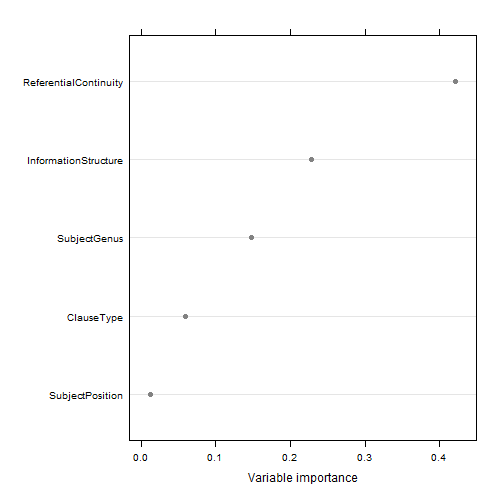
\includegraphics[width=3.125in,height=\textheight,keepaspectratio,alt={Dot plot showing the variable importance of five predictors in a Spanish native speaker subject realisation model. ReferentialContinuity has the highest variable importance, followed by InformationStructure, SubjectGenus, ClauseType, and SubjectPosition. The x-axis represents variable importance.}]{3_Extension1_GenderGenus/Figures/varimp_native_genus.png}

}

\caption{\label{fig-varimp-natives-closerepl1}Variable importance of the
Spanish native speaker model including \textsc{SubjectGenus}}

\end{figure}%

The variable importance of the L2 target-likeness model is shown in
Figure~\ref{fig-varimp-Germans-closerepl1}. The distribution is similar
to that of the original model, with \textsc{ReferentialContinuity} and
\textsc{SubjectType} by far the most influential variables, followed by
\textsc{ClauseType and SubjectPosition. SubjectGenus,
InformationStructure,} and \textsc{(Proficiency)Score} contribute little
to the model.

\begin{figure}

\centering{

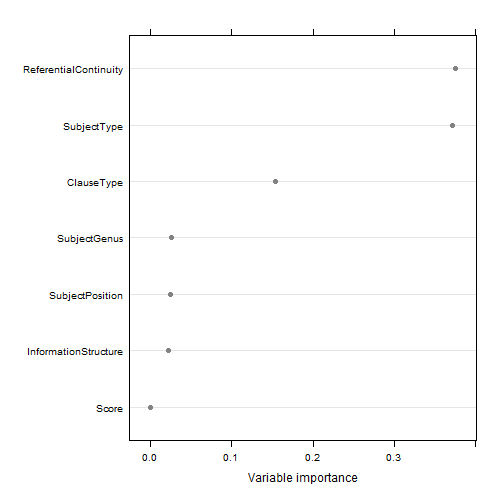
\includegraphics[width=3.125in,height=\textheight,keepaspectratio,alt={Dot plot showing the variable importance of seven predictors in an L2 Spanish subject realisation model. ReferentialContinuity has the highest variable importance, followed by SubjectType and ClauseType. SubjectGenus and SubjectPosition have lower and similar importance, followed by InformationStructure and Score. The x-axis represents variable importance.}]{3_Extension1_GenderGenus/Figures/varimp_l2.png}

}

\caption{\label{fig-varimp-Germans-closerepl1}Variable importance of the
random forest model of the TargetLinkeness of the L2 speakers.}

\end{figure}%

In total, 15 observations are classified incorrectly, compared with 11
in Kocher's original dataset:

\begin{longtable}[]{@{}lrr@{}}
\caption{Confusion matrix for the German L2 learners of Spanish data
including `SubjectGenus'. Rows indicate predicted subject types, columns
indicate actual subject types}\tabularnewline
\toprule\noalign{}
& FALSE & TRUE \\
\midrule\noalign{}
\endfirsthead
\toprule\noalign{}
& FALSE & TRUE \\
\midrule\noalign{}
\endhead
\bottomrule\noalign{}
\endlastfoot
FALSE & 875 & 1 \\
TRUE & 14 & 1973 \\
\end{longtable}

The final model for the extended L1 German learner dataset, including
\textsc{SubjectGenus}, achieves an accuracy of 99.5\%.

\subsubsection{Surrogate Decision Tree}\label{closerepli1_surro}

The proportion of correct predictions is higher for pronouns (40.7\%,
compared with 33.3\% in the robustness check without
\textsc{SubjectGenus}), while it is slightly lower for null subjects
(74.3\%, compared with 75.1\%) and DPs (72.9\%, compared with 77.3\%).
These differences are reflected in the surrogate tree shown in
Figure~\ref{fig-closerepl1-surro}.

\begin{figure}

\centering{

\pandocbounded{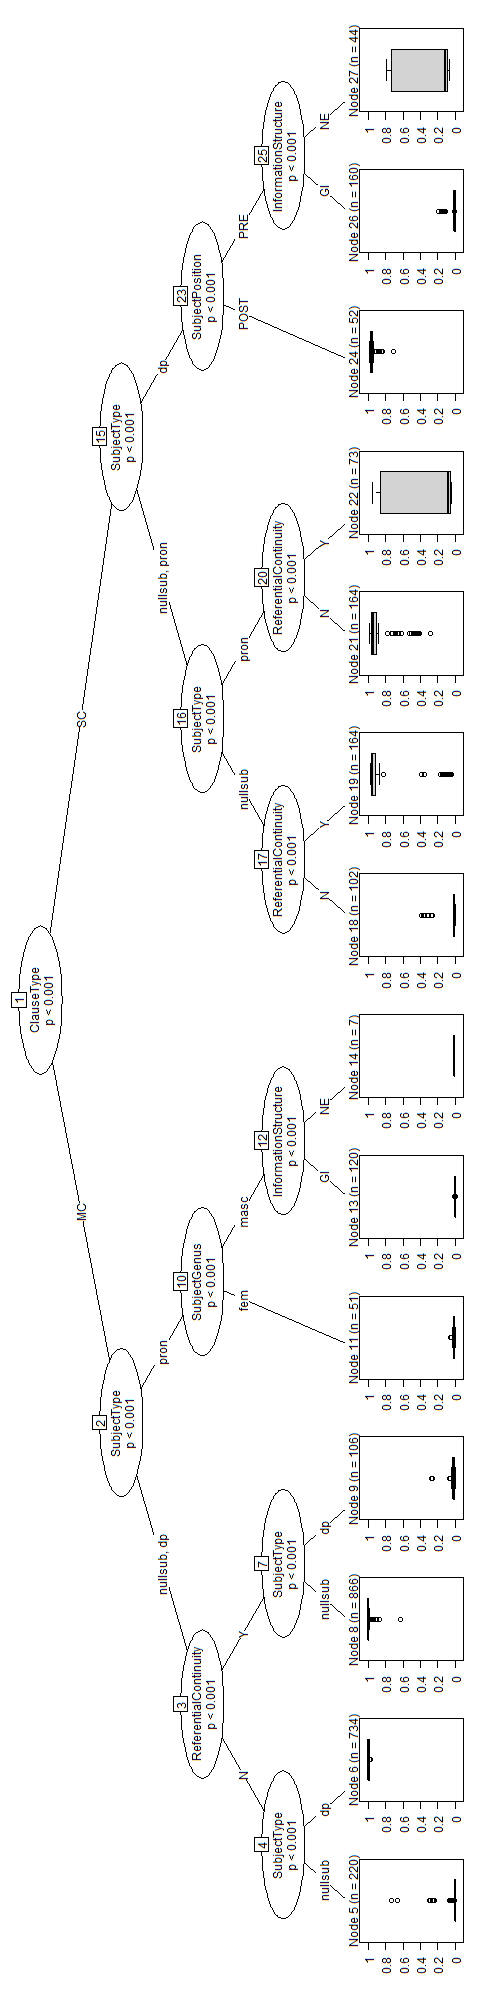
\includegraphics[keepaspectratio,alt={A recursive partitioning tree showing subject realisation among L1 German speakers. The first split is by ClauseType, separating main clauses (MC) from subordinate clauses (SC). The MC branch splits by SubjectType, followed by ReferentialContinuity and SubjectGenus for pronouns, and InformationStructure for null subjects. The SC branch splits by SubjectType into pronoun and nullsub, pron, with subsequent splits by SubjectPosition, InformationStructure, and ReferentialContinuity. Terminal nodes display distributions of the outcome variable, with sample sizes ranging from 1 to 866.}]{3_Extension1_GenderGenus/Figures/surro_l2german_landscape.png}}

}

\caption{\label{fig-closerepl1-surro}Surrogate tree of the random forest
model of the \textsc{TargetLikeness} of the L1 German learner of Spanish
(extended model including SubjectGnder).}

\end{figure}%

\newpage{}

The surrogate model has a high R² of 0.932, suggesting a good fit to the
data. On the left side of the tree, \textsc{ClauseType}, which separates
MCs from SCs, interacts with \textsc{SubjectType}. As in the previous
trees, null subjects and DPs are separated from pronouns. In MCs,
\textsc{ClauseType} and \textsc{SubjectType} interact with
\textsc{ReferentialContinuity, SubjectGenus,} and
\textsc{InformationStructure.} In SCs, they interact with
\textsc{SubjectPosition, InformationStructure,} and
\textsc{ReferentialContinuity}. In MCs, DPs are highly target-like when
used with discontinuous subjects (node 6), but are overused with
continuous subject referents (node 9). Conversely, null subjects are
highly target-like in continuous-subject contexts (node 8), as expected
given the prominence of continuity for null subject use. Null subjects
are, however, also overused in some discontinuous contexts (node 5). All
pronominal subjects used in MCs show low target-likeness, consistent
with the findings of the reproduction and robustness check. In the close
replication, pronouns interact with \textsc{SubjectGenus} (nodes 11-14)
and, for masculine referents, also with \textsc{InformationStructure}
(nodes 13-14).

In SCs, the tree separates null subjects and pronouns from DPs after
node 15, which differs from the previous trees, in which pronouns
behaved differently from the other two subject types. DPs in preverbal
position are generally used with low target-likeness, regardless of the
referent's \textsc{InformationStructure}. This is noteworthy given that
preverbal position is the default position for overt subjects. By
contrast, postverbal DPs are used with high target-likeness. Both null
subjects and pronouns in SCs interact with
\textsc{ReferentialContinuity}. Null subjects are highly target-like
with continuous subjects (node 19) but are overused with discontinuous
subjects. Pronouns, by contrast, are highly target-like with
discontinuous subjects (node 21) and slightly overused with continuous
subjects (node 22).

Overall, the L1 German model including \textsc{SubjectGenus} shows a
pattern similar to that observed in the previous surrogate trees, namely
that pronouns are generally overused, except in topic shift contexts in
SCs. At the same time, the interactions involving \textsc{SubjectGenus}
suggest that gender is relevant to the target-likeness of pronominal
subjects.

\subsection{Close replication 2: Gender inclusive model on L1 English
data}\label{close-replication-2-gender-inclusive-model-on-l1-english-data}

\subsubsection{Descriptive statistics of L1 English
data}\label{descriptive-statistics-of-l1-english-data}

In the L1 English speaker data, the distribution of subject types does
not differ significantly between speakers who know an additional NSL and
those who do not. This is also the case in Kocher's L1 German speaker
data.

\begin{longtable}[]{@{}
  >{\raggedright\arraybackslash}p{(\linewidth - 6\tabcolsep) * \real{0.5833}}
  >{\raggedright\arraybackslash}p{(\linewidth - 6\tabcolsep) * \real{0.1310}}
  >{\raggedright\arraybackslash}p{(\linewidth - 6\tabcolsep) * \real{0.1310}}
  >{\raggedright\arraybackslash}p{(\linewidth - 6\tabcolsep) * \real{0.1310}}@{}}
\caption{Proportion and frequency of subject type in the Spanish native
speaker and the L1 English learner of L2 Spanish
data.}\label{tbl-overview-frequencies-L2English}\tabularnewline
\toprule\noalign{}
\begin{minipage}[b]{\linewidth}\raggedright
\end{minipage} & \begin{minipage}[b]{\linewidth}\raggedright
dp
\end{minipage} & \begin{minipage}[b]{\linewidth}\raggedright
nullsub
\end{minipage} & \begin{minipage}[b]{\linewidth}\raggedright
pron
\end{minipage} \\
\midrule\noalign{}
\endfirsthead
\toprule\noalign{}
\begin{minipage}[b]{\linewidth}\raggedright
\end{minipage} & \begin{minipage}[b]{\linewidth}\raggedright
dp
\end{minipage} & \begin{minipage}[b]{\linewidth}\raggedright
nullsub
\end{minipage} & \begin{minipage}[b]{\linewidth}\raggedright
pron
\end{minipage} \\
\midrule\noalign{}
\endhead
\bottomrule\noalign{}
\endlastfoot
Spanish natives (L1), Kocher &
\begin{minipage}[t]{\linewidth}\raggedright
34.1\%\\
(178)\\
\strut
\end{minipage} & \begin{minipage}[t]{\linewidth}\raggedright
50\%\\
(261)\\
\strut
\end{minipage} & \begin{minipage}[t]{\linewidth}\raggedright
15.9\%\\
(83)\\
\strut
\end{minipage} \\
\begin{minipage}[t]{\linewidth}\raggedright
L1 German learners of\\
L2 Spanish (L2 German), extended Reproduction\strut
\end{minipage} & \begin{minipage}[t]{\linewidth}\raggedright
37.5\%\\
(1103)\\
\strut
\end{minipage} & \begin{minipage}[t]{\linewidth}\raggedright
47.2\%\\
(1389)\\
\strut
\end{minipage} & \begin{minipage}[t]{\linewidth}\raggedright
15.4\%\\
(453)\\
\strut
\end{minipage} \\
\begin{minipage}[t]{\linewidth}\raggedright
L1 English learners of\\
L2 Spanish (L2 English), extended Reproduction\strut
\end{minipage} & \begin{minipage}[t]{\linewidth}\raggedright
37.3\%\\
(470)\\
\strut
\end{minipage} & \begin{minipage}[t]{\linewidth}\raggedright
44.2\%\\
(557)\\
\strut
\end{minipage} & \begin{minipage}[t]{\linewidth}\raggedright
18.5\%\\
(233)\\
\strut
\end{minipage} \\
\end{longtable}

The overall distribution of DPs, null subjects, and pronouns does not
differ substantially from that of the Spanish native speaker and
extended L1 German learner datasets. In all three groups, null subjects
are the most frequent subject type, accounting for approximately half of
all subjects, while DPs account for around one third and pronouns are
used less frequently.

\begin{longtable}[]{@{}
  >{\raggedright\arraybackslash}p{(\linewidth - 12\tabcolsep) * \real{0.1757}}
  >{\centering\arraybackslash}p{(\linewidth - 12\tabcolsep) * \real{0.1216}}
  >{\centering\arraybackslash}p{(\linewidth - 12\tabcolsep) * \real{0.1216}}
  >{\centering\arraybackslash}p{(\linewidth - 12\tabcolsep) * \real{0.1351}}
  >{\centering\arraybackslash}p{(\linewidth - 12\tabcolsep) * \real{0.1351}}
  >{\centering\arraybackslash}p{(\linewidth - 12\tabcolsep) * \real{0.1216}}
  >{\centering\arraybackslash}p{(\linewidth - 12\tabcolsep) * \real{0.1216}}@{}}
\caption{Proportion and frequency of new versus given subjects by type
in the Spanish native speaker and the L1 English learner of L2 Spanish
data.}\label{tbl-info-structure-L2English}\tabularnewline
\toprule\noalign{}
\begin{minipage}[b]{\linewidth}\raggedright
\end{minipage} & \begin{minipage}[b]{\linewidth}\centering
dp
\end{minipage} & \begin{minipage}[b]{\linewidth}\centering
dp
\end{minipage} & \begin{minipage}[b]{\linewidth}\centering
nullsub
\end{minipage} & \begin{minipage}[b]{\linewidth}\centering
nullsub
\end{minipage} & \begin{minipage}[b]{\linewidth}\centering
pron
\end{minipage} & \begin{minipage}[b]{\linewidth}\centering
pron
\end{minipage} \\
\midrule\noalign{}
\endfirsthead
\toprule\noalign{}
\begin{minipage}[b]{\linewidth}\raggedright
\end{minipage} & \begin{minipage}[b]{\linewidth}\centering
dp
\end{minipage} & \begin{minipage}[b]{\linewidth}\centering
dp
\end{minipage} & \begin{minipage}[b]{\linewidth}\centering
nullsub
\end{minipage} & \begin{minipage}[b]{\linewidth}\centering
nullsub
\end{minipage} & \begin{minipage}[b]{\linewidth}\centering
pron
\end{minipage} & \begin{minipage}[b]{\linewidth}\centering
pron
\end{minipage} \\
\midrule\noalign{}
\endhead
\bottomrule\noalign{}
\endlastfoot
& Given & New & Given & New & Given & New \\
L1, Kocher & \begin{minipage}[t]{\linewidth}\centering
59.5\%\\
(106)\\
\strut
\end{minipage} & \begin{minipage}[t]{\linewidth}\centering
40.5\%\\
(72)\\
\strut
\end{minipage} & \begin{minipage}[t]{\linewidth}\centering
96.1\%\\
(248)\\
\strut
\end{minipage} & \begin{minipage}[t]{\linewidth}\centering
3.9\%\\
(10)\\
\strut
\end{minipage} & \begin{minipage}[t]{\linewidth}\centering
84.1\%\\
(69)\\
\strut
\end{minipage} & \begin{minipage}[t]{\linewidth}\centering
15.9\%\\
(13)\\
\strut
\end{minipage} \\
L2 German & \begin{minipage}[t]{\linewidth}\centering
72.3\%\\
(798)\\
\strut
\end{minipage} & \begin{minipage}[t]{\linewidth}\centering
27.6\%\\
(304)\\
\strut
\end{minipage} & \begin{minipage}[t]{\linewidth}\centering
97.2\%\\
(1350)\\
\strut
\end{minipage} & \begin{minipage}[t]{\linewidth}\centering
1.4\%\\
(20)\\
\strut
\end{minipage} & \begin{minipage}[t]{\linewidth}\centering
89.2\%\\
(404)\\
\strut
\end{minipage} & \begin{minipage}[t]{\linewidth}\centering
9.1\%\\
(41)\\
\strut
\end{minipage} \\
L2 English & \begin{minipage}[t]{\linewidth}\centering
77.9\%\\
(366)\strut
\end{minipage} & \begin{minipage}[t]{\linewidth}\centering
22.1\%\\
(104)\\
\strut
\end{minipage} & \begin{minipage}[t]{\linewidth}\centering
97.5\%\\
(543)\\
\strut
\end{minipage} & \begin{minipage}[t]{\linewidth}\centering
2.5\%\\
(14)\\
\strut
\end{minipage} & \begin{minipage}[t]{\linewidth}\centering
97.9\%\\
(228)\\
\strut
\end{minipage} & \begin{minipage}[t]{\linewidth}\centering
2.1\%\\
(5)\\
\strut
\end{minipage} \\
\end{longtable}

The distribution of new and given referents in the L1 English learner
data differs slightly from that observed in Kocher's data and the L1
German learner data (\citeproc{ref-kocher_subject_2025}{2025}: 16). L1
English learners realise DPs predominantly with given referents, even
more strongly than the L1 German learners and Spanish native speakers.
They also use pronouns more exclusively with given referents than the
other two groups. The association between \textsc{SubjectType} and
\textsc{InformationStructure} is statistically significant (X² = 130.15,
\emph{p} \textless{} 0.001).

\begin{longtable}[]{@{}
  >{\raggedright\arraybackslash}p{(\linewidth - 12\tabcolsep) * \real{0.1238}}
  >{\centering\arraybackslash}p{(\linewidth - 12\tabcolsep) * \real{0.1238}}
  >{\centering\arraybackslash}p{(\linewidth - 12\tabcolsep) * \real{0.1524}}
  >{\centering\arraybackslash}p{(\linewidth - 12\tabcolsep) * \real{0.1238}}
  >{\centering\arraybackslash}p{(\linewidth - 12\tabcolsep) * \real{0.1524}}
  >{\centering\arraybackslash}p{(\linewidth - 12\tabcolsep) * \real{0.1238}}
  >{\centering\arraybackslash}p{(\linewidth - 12\tabcolsep) * \real{0.1524}}@{}}
\caption{Proportion and frequency of (dis-)continuous referents by type
in the Spanish native speaker, the extended L1 German and L1 English
learner of L2 Spanish
data.}\label{tbl-referential-continuity-L2English}\tabularnewline
\toprule\noalign{}
\begin{minipage}[b]{\linewidth}\raggedright
\end{minipage} & \begin{minipage}[b]{\linewidth}\centering
dp
\end{minipage} & \begin{minipage}[b]{\linewidth}\centering
dp
\end{minipage} & \begin{minipage}[b]{\linewidth}\centering
nullsub
\end{minipage} & \begin{minipage}[b]{\linewidth}\centering
nullsub
\end{minipage} & \begin{minipage}[b]{\linewidth}\centering
pron
\end{minipage} & \begin{minipage}[b]{\linewidth}\centering
pron
\end{minipage} \\
\midrule\noalign{}
\endfirsthead
\toprule\noalign{}
\begin{minipage}[b]{\linewidth}\raggedright
\end{minipage} & \begin{minipage}[b]{\linewidth}\centering
dp
\end{minipage} & \begin{minipage}[b]{\linewidth}\centering
dp
\end{minipage} & \begin{minipage}[b]{\linewidth}\centering
nullsub
\end{minipage} & \begin{minipage}[b]{\linewidth}\centering
nullsub
\end{minipage} & \begin{minipage}[b]{\linewidth}\centering
pron
\end{minipage} & \begin{minipage}[b]{\linewidth}\centering
pron
\end{minipage} \\
\midrule\noalign{}
\endhead
\bottomrule\noalign{}
\endlastfoot
& Continuous & Discontinuous & Continuous & Discontinuous & Continuous &
Discontinuous \\
L1, Kocher & \begin{minipage}[t]{\linewidth}\centering
9\%\\
(16)\\
\strut
\end{minipage} & \begin{minipage}[t]{\linewidth}\centering
91\%\\
(162)\\
\strut
\end{minipage} & \begin{minipage}[t]{\linewidth}\centering
61.5\%\\
(158)\\
\strut
\end{minipage} & \begin{minipage}[t]{\linewidth}\centering
38.5\%\\
(99)\\
\strut
\end{minipage} & \begin{minipage}[t]{\linewidth}\centering
29\%\\
(24)\\
\strut
\end{minipage} & \begin{minipage}[t]{\linewidth}\centering
71\%\\
(59)\\
\strut
\end{minipage} \\
L2 German & \begin{minipage}[t]{\linewidth}\centering
11\%\\
(121)\\
\strut
\end{minipage} & \begin{minipage}[t]{\linewidth}\centering
89\%\\
(982)\\
\strut
\end{minipage} & \begin{minipage}[t]{\linewidth}\centering
75\%\\
(1042)\\
\strut
\end{minipage} & \begin{minipage}[t]{\linewidth}\centering
24.3\%\\
(337)\\
\strut
\end{minipage} & \begin{minipage}[t]{\linewidth}\centering
33.6\%\\
(152)\\
\strut
\end{minipage} & \begin{minipage}[t]{\linewidth}\centering
66.4\%\\
(301)\\
\strut
\end{minipage} \\
L2 English & \begin{minipage}[t]{\linewidth}\centering
18.3\%\\
(86)\\
\strut
\end{minipage} & \begin{minipage}[t]{\linewidth}\centering
81.7\%\\
(384)\\
\strut
\end{minipage} & \begin{minipage}[t]{\linewidth}\centering
74.5\%\\
(415)\\
\strut
\end{minipage} & \begin{minipage}[t]{\linewidth}\centering
25.5\%\\
(142)\\
\strut
\end{minipage} & \begin{minipage}[t]{\linewidth}\centering
35.2\%\\
(82)\\
\strut
\end{minipage} & \begin{minipage}[t]{\linewidth}\centering
64.8\%\\
(151)\\
\strut
\end{minipage} \\
\end{longtable}

The distribution of continuous and discontinuous referents likewise
differs only slightly from that of the Spanish native speaker and L1
German learner data. As in the other groups, DPs and pronouns are
predominantly used for discontinuous referents, whereas null subjects
are mainly used for continuous referents. However, the use of null
subjects and pronouns is more evenly distributed across continuous and
discontinuous contexts in the L1 English data than in the DP data. These
differences are statistically significant (X² = 338.05, \emph{p}
\textless{} 0.001).

\begin{longtable}[]{@{}
  >{\raggedright\arraybackslash}p{(\linewidth - 12\tabcolsep) * \real{0.1757}}
  >{\centering\arraybackslash}p{(\linewidth - 12\tabcolsep) * \real{0.1216}}
  >{\centering\arraybackslash}p{(\linewidth - 12\tabcolsep) * \real{0.1216}}
  >{\centering\arraybackslash}p{(\linewidth - 12\tabcolsep) * \real{0.1351}}
  >{\centering\arraybackslash}p{(\linewidth - 12\tabcolsep) * \real{0.1351}}
  >{\centering\arraybackslash}p{(\linewidth - 12\tabcolsep) * \real{0.1216}}
  >{\centering\arraybackslash}p{(\linewidth - 12\tabcolsep) * \real{0.1216}}@{}}
\caption{Proportion and frequency of MCs versus SCs by type in the
Spanish native speaker, the L1 German and L1 English learner of L2
Spanish data.}\label{tbl-clause-type-L2English}\tabularnewline
\toprule\noalign{}
\begin{minipage}[b]{\linewidth}\raggedright
\end{minipage} & \begin{minipage}[b]{\linewidth}\centering
dp
\end{minipage} & \begin{minipage}[b]{\linewidth}\centering
dp
\end{minipage} & \begin{minipage}[b]{\linewidth}\centering
nullsub
\end{minipage} & \begin{minipage}[b]{\linewidth}\centering
nullsub
\end{minipage} & \begin{minipage}[b]{\linewidth}\centering
pron
\end{minipage} & \begin{minipage}[b]{\linewidth}\centering
pron
\end{minipage} \\
\midrule\noalign{}
\endfirsthead
\toprule\noalign{}
\begin{minipage}[b]{\linewidth}\raggedright
\end{minipage} & \begin{minipage}[b]{\linewidth}\centering
dp
\end{minipage} & \begin{minipage}[b]{\linewidth}\centering
dp
\end{minipage} & \begin{minipage}[b]{\linewidth}\centering
nullsub
\end{minipage} & \begin{minipage}[b]{\linewidth}\centering
nullsub
\end{minipage} & \begin{minipage}[b]{\linewidth}\centering
pron
\end{minipage} & \begin{minipage}[b]{\linewidth}\centering
pron
\end{minipage} \\
\midrule\noalign{}
\endhead
\bottomrule\noalign{}
\endlastfoot
& MC & SC & MC & SC & MC & SC \\
L1, Kocher & \begin{minipage}[t]{\linewidth}\centering
75.8\%\\
(135)\\
\strut
\end{minipage} & \begin{minipage}[t]{\linewidth}\centering
24.2\%\\
(43)\\
\strut
\end{minipage} & \begin{minipage}[t]{\linewidth}\centering
72\%\\
(188)\\
\strut
\end{minipage} & \begin{minipage}[t]{\linewidth}\centering
28\%\\
(73)\\
\strut
\end{minipage} & \begin{minipage}[t]{\linewidth}\centering
26.5\%\\
(22)\\
\strut
\end{minipage} & \begin{minipage}[t]{\linewidth}\centering
73.5\%\\
(61)\\
\strut
\end{minipage} \\
L2 German & \begin{minipage}[t]{\linewidth}\centering
76.8\%\\
(847)\\
\strut
\end{minipage} & \begin{minipage}[t]{\linewidth}\centering
23.2\%\\
(256)\\
\strut
\end{minipage} & \begin{minipage}[t]{\linewidth}\centering
79.9\%\\
(1110)\\
\strut
\end{minipage} & \begin{minipage}[t]{\linewidth}\centering
20.1\%\\
(279)\\
\strut
\end{minipage} & \begin{minipage}[t]{\linewidth}\centering
42.8\%\\
(194)\\
\strut
\end{minipage} & \begin{minipage}[t]{\linewidth}\centering
57.2\%\\
(259)\\
\strut
\end{minipage} \\
L2 English & \begin{minipage}[t]{\linewidth}\centering
85.3\%\\
(401)\\
\strut
\end{minipage} & \begin{minipage}[t]{\linewidth}\centering
14.7\%\\
(69)\\
\strut
\end{minipage} & \begin{minipage}[t]{\linewidth}\centering
77\%\\
(429)\\
\strut
\end{minipage} & \begin{minipage}[t]{\linewidth}\centering
23\%\\
(128)\\
\strut
\end{minipage} & \begin{minipage}[t]{\linewidth}\centering
57.9\%\\
(135)\\
\strut
\end{minipage} & \begin{minipage}[t]{\linewidth}\centering
42.1\%\\
(98)\\
\strut
\end{minipage} \\
\end{longtable}

The distribution across MCs and SCs also differs between the L1 English
and L1 German learner data. The main difference concerns pronoun use.
Unlike the L1 German learners and Spanish native speakers, the L1
English learners use pronouns more evenly across MCs and SCs, although
pronouns still occur more frequently in MCs. DPs are predominantly
realised in MCs, whereas the distribution of null subjects is more
similar to that of the Spanish native speakers. The differences between
\textsc{SubjectType} and \textsc{ClauseType} are statistically
significant (X² = 251.21, \emph{p} \textless{} 0.001).

\begin{longtable}[]{@{}
  >{\raggedright\arraybackslash}p{(\linewidth - 8\tabcolsep) * \real{0.1806}}
  >{\centering\arraybackslash}p{(\linewidth - 8\tabcolsep) * \real{0.1667}}
  >{\centering\arraybackslash}p{(\linewidth - 8\tabcolsep) * \real{0.1806}}
  >{\centering\arraybackslash}p{(\linewidth - 8\tabcolsep) * \real{0.1667}}
  >{\centering\arraybackslash}p{(\linewidth - 8\tabcolsep) * \real{0.1806}}@{}}
\caption{Proportion and frequency of pre- and postverbal subjects by
type in the Spanish native speaker, the L1 German and L1 English learner
of L2 Spanish
data.}\label{tbl-subject-position-L2English}\tabularnewline
\toprule\noalign{}
\begin{minipage}[b]{\linewidth}\raggedright
\end{minipage} & \begin{minipage}[b]{\linewidth}\centering
dp
\end{minipage} & \begin{minipage}[b]{\linewidth}\centering
dp
\end{minipage} & \begin{minipage}[b]{\linewidth}\centering
pron
\end{minipage} & \begin{minipage}[b]{\linewidth}\centering
pron
\end{minipage} \\
\midrule\noalign{}
\endfirsthead
\toprule\noalign{}
\begin{minipage}[b]{\linewidth}\raggedright
\end{minipage} & \begin{minipage}[b]{\linewidth}\centering
dp
\end{minipage} & \begin{minipage}[b]{\linewidth}\centering
dp
\end{minipage} & \begin{minipage}[b]{\linewidth}\centering
pron
\end{minipage} & \begin{minipage}[b]{\linewidth}\centering
pron
\end{minipage} \\
\midrule\noalign{}
\endhead
\bottomrule\noalign{}
\endlastfoot
& Preverbal & Postverbal & Preverbal & Postverbal \\
L1, Kocher & \begin{minipage}[t]{\linewidth}\centering
77.5\%\\
(138)\\
\strut
\end{minipage} & \begin{minipage}[t]{\linewidth}\centering
22.5\%\\
(40)\\
\strut
\end{minipage} & \begin{minipage}[t]{\linewidth}\centering
95\%\\
(77)\\
\strut
\end{minipage} & \begin{minipage}[t]{\linewidth}\centering
5\%\\
(4)\\
\strut
\end{minipage} \\
L2 German & \begin{minipage}[t]{\linewidth}\centering
86.3\%\\
(934)\\
\strut
\end{minipage} & \begin{minipage}[t]{\linewidth}\centering
13.7\%\\
(148)\\
\strut
\end{minipage} & \begin{minipage}[t]{\linewidth}\centering
96.1\%\\
(423)\\
\strut
\end{minipage} & \begin{minipage}[t]{\linewidth}\centering
3.9\%\\
(17)\\
\strut
\end{minipage} \\
L2 English & \begin{minipage}[t]{\linewidth}\centering
96.4\%\\
(453)\\
\strut
\end{minipage} & \begin{minipage}[t]{\linewidth}\centering
3.6\%\\
(17)\\
\strut
\end{minipage} & \begin{minipage}[t]{\linewidth}\centering
99.1\%\\
(231)\\
\strut
\end{minipage} & \begin{minipage}[t]{\linewidth}\centering
0.9\%\\
(2)\\
\strut
\end{minipage} \\
\end{longtable}

The distribution of subject position is also similar to that of Kocher's
dataset, although the L1 English data show a clearer distinction between
preverbal and postverbal subjects. As preverbal position is the unmarked
position for subjects with most Spanish verbs, both subject types are
expected to occur predominantly in this position (see
\citeproc{ref-kocher_subject_2025}{2025}: 17). In contrast to the
Spanish native speaker and L1 German groups, the L1 English learners
realise pronouns exclusively preverbally. They also use DPs more
frequently in preverbal position than the other groups. However, these
differences are not statistically significant (X² = 3.5201, \emph{p}
\textgreater{} 0.05). As in the extended L2 German dataset, most
postverbal cases in the L1 English data occur with presentative
\emph{ser} and unaccusative verbs such as \emph{venir, aparecer, pasar,
caer,} and \emph{estar} (compare
\citeproc{ref-kocher_subject_2025}{Kocher, 2025}: 18).

\begin{longtable}[]{@{}
  >{\raggedright\arraybackslash}p{(\linewidth - 18\tabcolsep) * \real{0.1000}}
  >{\raggedright\arraybackslash}p{(\linewidth - 18\tabcolsep) * \real{0.1000}}
  >{\raggedright\arraybackslash}p{(\linewidth - 18\tabcolsep) * \real{0.1000}}
  >{\raggedright\arraybackslash}p{(\linewidth - 18\tabcolsep) * \real{0.1000}}
  >{\raggedright\arraybackslash}p{(\linewidth - 18\tabcolsep) * \real{0.1000}}
  >{\raggedright\arraybackslash}p{(\linewidth - 18\tabcolsep) * \real{0.1000}}
  >{\raggedright\arraybackslash}p{(\linewidth - 18\tabcolsep) * \real{0.1000}}
  >{\raggedright\arraybackslash}p{(\linewidth - 18\tabcolsep) * \real{0.1000}}
  >{\raggedright\arraybackslash}p{(\linewidth - 18\tabcolsep) * \real{0.1000}}
  >{\raggedright\arraybackslash}p{(\linewidth - 18\tabcolsep) * \real{0.1000}}@{}}
\caption{Proportion and frequency of masculine and feminine subjects by
type in the Spanish native speaker, the L1 English and L1 German learner
of L2 Spanish data.}\label{tbl-genus-L1English}\tabularnewline
\toprule\noalign{}
\begin{minipage}[b]{\linewidth}\raggedright
\end{minipage} & \begin{minipage}[b]{\linewidth}\raggedright
masc
\end{minipage} & \begin{minipage}[b]{\linewidth}\raggedright
masc
\end{minipage} & \begin{minipage}[b]{\linewidth}\raggedright
masc
\end{minipage} & \begin{minipage}[b]{\linewidth}\raggedright
fem
\end{minipage} & \begin{minipage}[b]{\linewidth}\raggedright
fem
\end{minipage} & \begin{minipage}[b]{\linewidth}\raggedright
fem
\end{minipage} & \begin{minipage}[b]{\linewidth}\raggedright
un-known
\end{minipage} & \begin{minipage}[b]{\linewidth}\raggedright
un-known
\end{minipage} & \begin{minipage}[b]{\linewidth}\raggedright
un-known
\end{minipage} \\
\midrule\noalign{}
\endfirsthead
\toprule\noalign{}
\begin{minipage}[b]{\linewidth}\raggedright
\end{minipage} & \begin{minipage}[b]{\linewidth}\raggedright
masc
\end{minipage} & \begin{minipage}[b]{\linewidth}\raggedright
masc
\end{minipage} & \begin{minipage}[b]{\linewidth}\raggedright
masc
\end{minipage} & \begin{minipage}[b]{\linewidth}\raggedright
fem
\end{minipage} & \begin{minipage}[b]{\linewidth}\raggedright
fem
\end{minipage} & \begin{minipage}[b]{\linewidth}\raggedright
fem
\end{minipage} & \begin{minipage}[b]{\linewidth}\raggedright
un-known
\end{minipage} & \begin{minipage}[b]{\linewidth}\raggedright
un-known
\end{minipage} & \begin{minipage}[b]{\linewidth}\raggedright
un-known
\end{minipage} \\
\midrule\noalign{}
\endhead
\bottomrule\noalign{}
\endlastfoot
& dp & nullsub & pron & dp & nullsub & pron & dp & nullsub & pron \\
L1 & 71.8\% (127) & 86.4\% (223) & 59\% (49) & 27.1\% (48) & 10.5\
& 28.9\% (24) & 1.1\% (2) & 3.1\% (8) & 12\% (10) \\
L2 German & 74.8\% (822) & 85.2\% (1167) & 61.4\% (278) & 24.9\% (274) &
13.5\% (185) & 30.2\% (137) & 0.3\% (3) & 1.3\% (18) & 8.4\% (38) \\
L2 English & 76.4\% (359) & 88.5\% (493) & 67.4\% (157) & 23.6\% (111) &
11.5\% (64) & 32.6\% (76) & 0\% (0) & 0\% (0) & 0\% (0) \\
\end{longtable}

The overall comparison shows that subjects are masculine in 77.0\% of
the L1 Spanish data, 77.6\% of the L1 German data, and 80\% of the L1
English data. The distribution of masculine and feminine referents
across subject types in the L1 English data is similar to that observed
in the other two groups (see Table~\ref{tbl-genus-L1English}). Between
85.2\% and 88.5\% of masculine subjects are realised as null subjects,
whereas approximately half of feminine referents are realised as DPs. In
both learner datasets, subjects whose referents cannot be identified are
preferably realised as pronouns, but also occur as null subjects. The
association between \textsc{SubjectGenus} and \textsc{SubjectType} is
statistically significant in the L1 English data (X² = 52.39, \emph{p}
\textless{} 0.001).

\begin{longtable}[]{@{}
  >{\raggedright\arraybackslash}p{(\linewidth - 12\tabcolsep) * \real{0.1733}}
  >{\centering\arraybackslash}p{(\linewidth - 12\tabcolsep) * \real{0.1200}}
  >{\centering\arraybackslash}p{(\linewidth - 12\tabcolsep) * \real{0.1200}}
  >{\centering\arraybackslash}p{(\linewidth - 12\tabcolsep) * \real{0.1333}}
  >{\centering\arraybackslash}p{(\linewidth - 12\tabcolsep) * \real{0.1333}}
  >{\centering\arraybackslash}p{(\linewidth - 12\tabcolsep) * \real{0.1200}}
  >{\centering\arraybackslash}p{(\linewidth - 12\tabcolsep) * \real{0.1333}}@{}}
\caption{Proportion and frequency of masculine and feminine subjects by
the speaker's gender in the Spanish native speaker and the L1 German
learner of L2 Spanish
data.}\label{tbl-SpeakerGender-L1Engl}\tabularnewline
\toprule\noalign{}
\begin{minipage}[b]{\linewidth}\raggedright
\end{minipage} & \begin{minipage}[b]{\linewidth}\centering
Male
\end{minipage} & \begin{minipage}[b]{\linewidth}\centering
Male
\end{minipage} & \begin{minipage}[b]{\linewidth}\centering
Male
\end{minipage} & \begin{minipage}[b]{\linewidth}\centering
Female
\end{minipage} & \begin{minipage}[b]{\linewidth}\centering
Female
\end{minipage} & \begin{minipage}[b]{\linewidth}\centering
Female
\end{minipage} \\
\midrule\noalign{}
\endfirsthead
\toprule\noalign{}
\begin{minipage}[b]{\linewidth}\raggedright
\end{minipage} & \begin{minipage}[b]{\linewidth}\centering
Male
\end{minipage} & \begin{minipage}[b]{\linewidth}\centering
Male
\end{minipage} & \begin{minipage}[b]{\linewidth}\centering
Male
\end{minipage} & \begin{minipage}[b]{\linewidth}\centering
Female
\end{minipage} & \begin{minipage}[b]{\linewidth}\centering
Female
\end{minipage} & \begin{minipage}[b]{\linewidth}\centering
Female
\end{minipage} \\
\midrule\noalign{}
\endhead
\bottomrule\noalign{}
\endlastfoot
& masc & fem & unknown & masc & fem & unknown \\
L1 & \begin{minipage}[t]{\linewidth}\centering
77\%\\
(154)\\
\strut
\end{minipage} & \begin{minipage}[t]{\linewidth}\centering
19.5\%\\
(39)\\
\strut
\end{minipage} & \begin{minipage}[t]{\linewidth}\centering
3.5\%\\
(7)\\
\strut
\end{minipage} & \begin{minipage}[t]{\linewidth}\centering
77\%\\
(245)\\
\strut
\end{minipage} & \begin{minipage}[t]{\linewidth}\centering
18.9\%\\
(60)\\
\strut
\end{minipage} & \begin{minipage}[t]{\linewidth}\centering
4.1\%\\
(13)\\
\strut
\end{minipage} \\
L2 German & \begin{minipage}[t]{\linewidth}\centering
80\%\\
(411)\\
\strut
\end{minipage} & \begin{minipage}[t]{\linewidth}\centering
19.3\%\\
(99)\\
\strut
\end{minipage} & \begin{minipage}[t]{\linewidth}\centering
0.8\%\\
(4)\\
\strut
\end{minipage} & \begin{minipage}[t]{\linewidth}\centering
77.1\%\\
(1856)\\
\strut
\end{minipage} & \begin{minipage}[t]{\linewidth}\centering
20.6\%\\
(497)\\
\strut
\end{minipage} & \begin{minipage}[t]{\linewidth}\centering
2.3\%\\
(55)\\
\strut
\end{minipage} \\
L2 English & \begin{minipage}[t]{\linewidth}\centering
80.2\%\\
(280)\\
\strut
\end{minipage} & \begin{minipage}[t]{\linewidth}\centering
19.8\%\\
(69)\\
\strut
\end{minipage} & \begin{minipage}[t]{\linewidth}\centering
0\%\\
(0)\\
\strut
\end{minipage} & \begin{minipage}[t]{\linewidth}\centering
80\%\\
(729)\\
\strut
\end{minipage} & \begin{minipage}[t]{\linewidth}\centering
20\%\\
(182)\\
\strut
\end{minipage} & \begin{minipage}[t]{\linewidth}\centering
0\%\\
(0)\\
\strut
\end{minipage} \\
\end{longtable}

The distribution of subject genus by speaker gender in the L1 English
learner data likewise supports the male gender bias reported by Da Cunha
for both male and female speakers (\citeproc{ref-dacunha2024}{2024}:
189). As in the Spanish native speaker and L1 German data, female
speakers do not show a ``biais nul'' but use masculine subjects as
frequently as male speakers (see \citeproc{ref-dacunha2024}{2024}: 194).
The differences are not statistically significant (X² = 1.316e-05,
\emph{p} \textgreater{} 0.05). The (Proficiency)Scores of each L1
English learners of L2 Spanish from the corpus are displayed below:

\begin{figure}[H]

{\centering 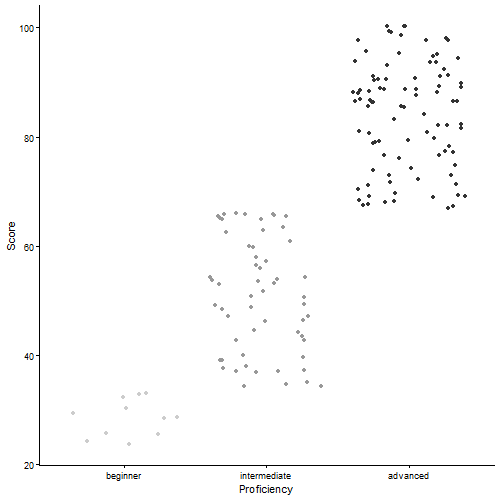
\includegraphics[width=2.60417in,height=\textheight,keepaspectratio]{4_Extension2_EnglishGenus/Figures/Scores.png}

}

\caption{Placement score of each English speaker of L2 Spanish, light
gray: beginners (\textless33), gray: intermediate (33\textgreater66),
black: advanced (\textgreater66).}

\end{figure}%

There are more beginner-level participants among the L1 English learners
(\emph{N} = 11) than in the L1 German dataset (see
Figure~\ref{fig-scores-german-extended}). However, the L1 English
dataset is likewise right-skewed towards intermediate (\emph{N} = 57)
and advanced learners (\emph{N} = 92).

\subsubsection{Variable importance and model accuracy of the L1 English
speaker
data}\label{variable-importance-and-model-accuracy-of-the-l1-english-speaker-data}

The L1 English learners show a distribution of correct predictions
similar to that of the L1 German learners in the first close
replication. While 67.8\% of null subjects are predicted correctly
(65.6\% in the extended L1 German dataset), the corresponding figure for
DPs is 72.1\% (75.8\% in the L1 German dataset). Pronouns appear to be
the most problematic subject type, with only 22.2\% predicted correctly,
compared with 50.6\% in the L1 German dataset from the first close
replication. The variable importance of the \textsc{target-likeness}
model for the L1 English learners of L2 Spanish is shown in
Figure~\ref{fig-varimp-l2English} below.

\begin{figure}

\centering{

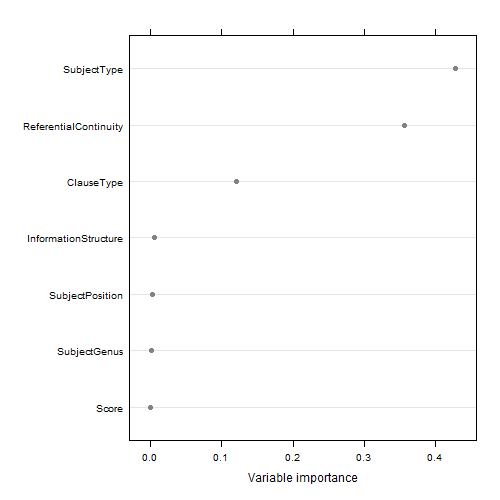
\includegraphics[width=3.125in,height=\textheight,keepaspectratio,alt={Dot plot showing the variable importance of seven predictors in an L1 English subject realisation model. SubjectType has the highest variable importance, followed by ReferentialContinuity and ClauseType. InformationStructure and SubjectPosition have lower importance, while SubjectGenus and Score have very low importance. The x-axis represents variable importance.}]{4_Extension2_EnglishGenus/Figures/varimp_EnglishL1.png}

}

\caption{\label{fig-varimp-l2English}Variable importance of the random
forest model of the \textsc{TargetLinkeness} of the L1 English learners
of L2 Spanish.}

\end{figure}%

The variable importance plot shows a distribution similar to that of the
L1 German model, with \textsc{SubjectType} and
\textsc{ReferentialContinuity} by far the most influential variables,
followed by \textsc{ClauseType. InformationStructure, SubjectGenus,
(Proficiency)Score,} and \textsc{SubjectPosition} contribute little to
the model. The confusion matrix of the L1 English learner model is
presented below.

{

\begin{longtable}[]{@{}lrr@{}}

\caption{\label{tbl-model-accuracy-closerepl2}Reproduced confusion
matrix for the L1 English learner of Spanish. Rows indicate predicted
subject types, columns indicate actual subject types}

\tabularnewline

\toprule\noalign{}
& FALSE & TRUE \\
\midrule\noalign{}
\endhead
\bottomrule\noalign{}
\endlastfoot
FALSE & 422 & 10 \\
TRUE & 8 & 820 \\

\end{longtable}

}

The L1 English learner model achieves an accuracy of 98.6\%, which is
similarly high to that of the L1 German learner model. In total, 18
observations are classified incorrectly.

\subsubsection{Surrogate Decision Tree}\label{surrogate-decision-tree}

The proportion of correct predictions is lowest for pronouns (41\%),
similar to the L1 German learners taken from the first close replication
(40.7\%). Target-likeness is highest for null subjects (73.6\%, compared
with 74.3\% for the L1 German learners), followed by DPs (72.1\%,
compared with 72.9\% for the L1 German learners). These patterns are
reflected in the surrogate tree for the L1 English learners (see
Figure~\ref{fig-surro-closerepl2}).

\begin{figure}

\centering{

\pandocbounded{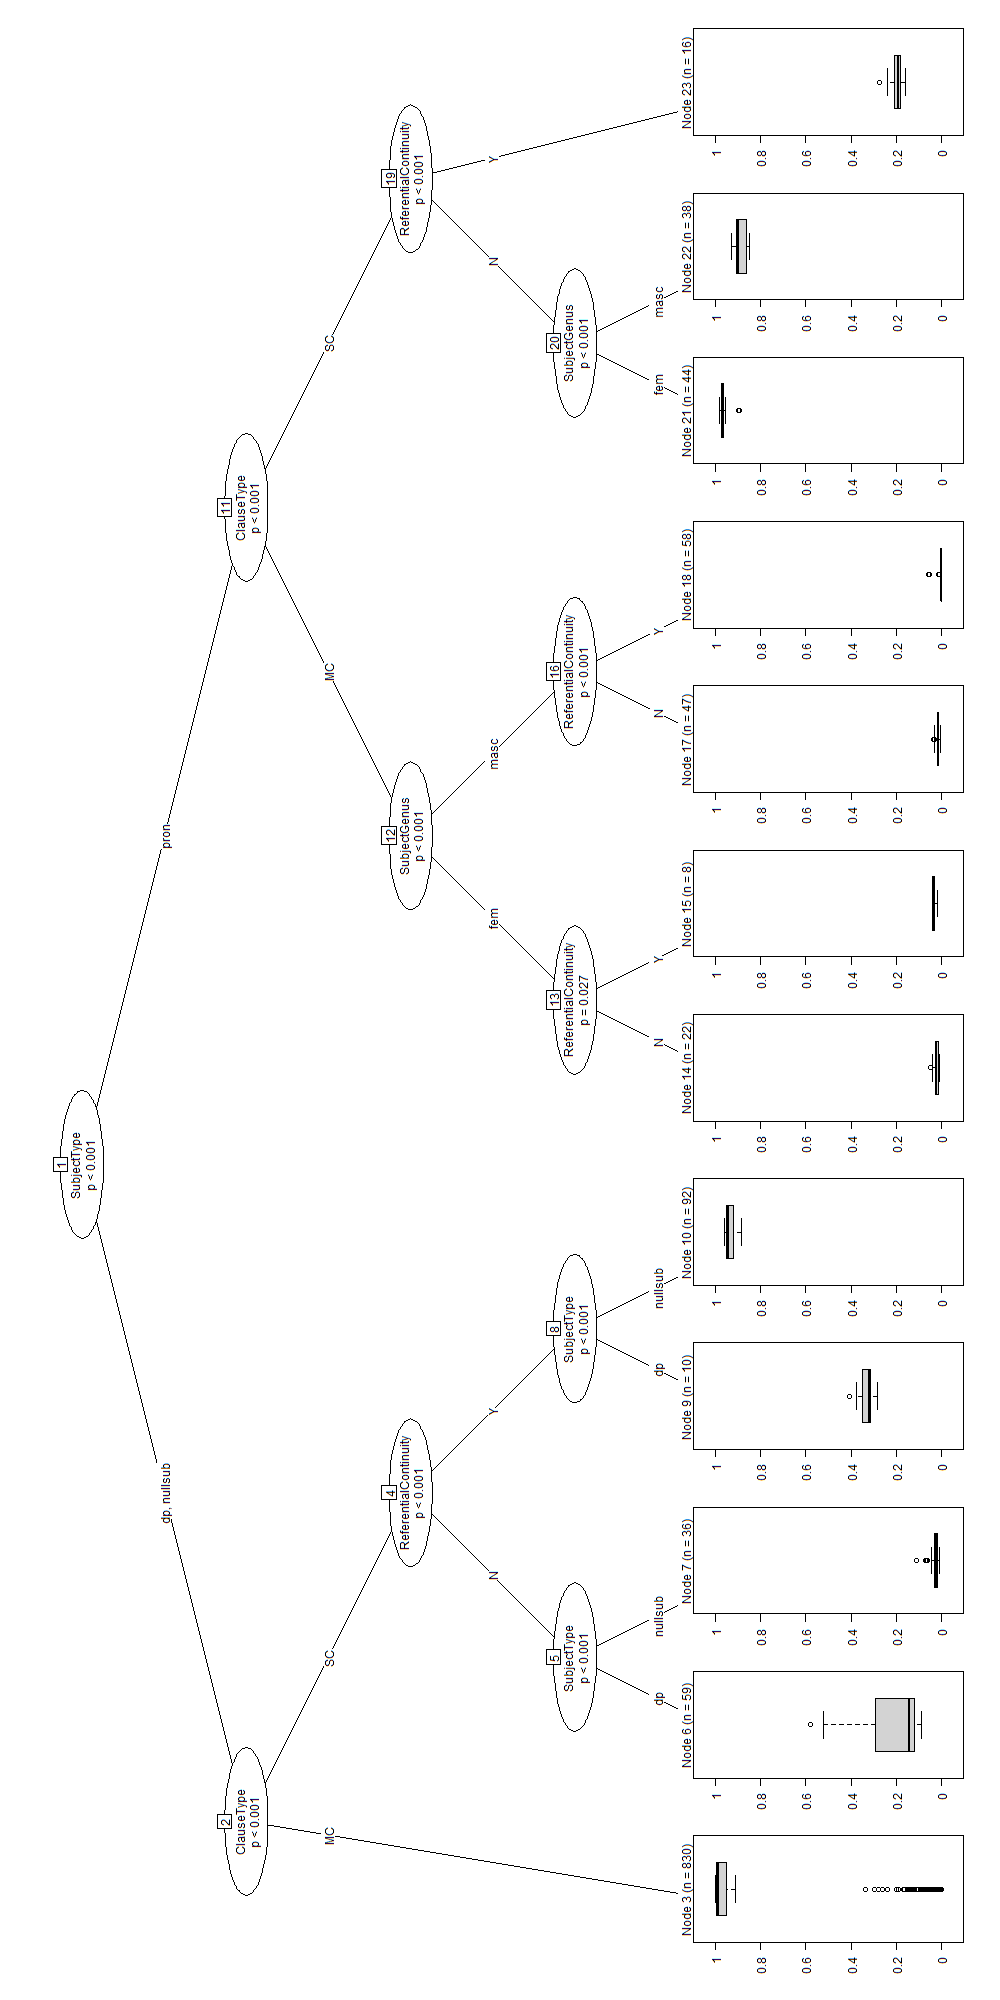
\includegraphics[keepaspectratio,alt={A recursive partitioning tree showing subject realisation in the L2 English speaker data. The first split is by SubjectType, separating pronoun from dp, nullsub. The pronoun branch is then split by ClauseType into main clauses (MC) and subordinate clauses (SC). In the MC branch, SubjectGenus and ReferentialContinuity further divide the data; in the SC branch, ReferentialContinuity is followed by SubjectGenus. The dp, nullsub branch is split by ClauseType; its SC branch is further divided by ReferentialContinuity and SubjectType. Terminal nodes display distributions of the outcome variable, with sample sizes ranging from 8 to 830.}]{4_Extension2_EnglishGenus/Figures/surro_l2English_landscape.png}}

}

\caption{\label{fig-surro-closerepl2}Surrogate tree of the random forest
model of the TargetLikeness of the L1 English learner of Spanish
(extended model including SubjectGender).}

\end{figure}%

\newpage{}

The L1 English surrogate tree has an R² of 0.467, suggesting a moderate
fit to the model. It shows that \textsc{SubjectType} and
\textsc{ClauseType} enter into complex interactions with
\textsc{ReferentialContinuity} for null subjects and DPs, while
\textsc{SubjectGenus} also enters into the interaction for pronominal
subjects. Specifically, L1 English learners of L2 Spanish show
target-like use of null subjects and DPs in MCs (node 3), whereas in SCs
this is only the case for continuous null subjects (node 10). The
learners show difficulties with DP use in SCs, reflected in their low
target-likeness with both continuous and discontinuous subjects (nodes 6
and 9). This overuse occurs with both continuous and discontinuous
referents (nodes 6 and 9). It is also associated with the overuse of
null subjects with discontinuous referents (node 7), a context in which
Spanish native speakers likewise do not tend to use null subjects.

After the first right-hand branch splits pronouns from null subjects and
DPs (node 11), \textsc{SubjectType} and \textsc{ClauseType} interact
with \textsc{SubjectGenus and ReferentialContinuity}. The only
target-like use of pronouns occurs in SCs with discontinuous referents,
regardless of \textsc{SubjectGenus} (nodes 21 and 22). This pattern is
related to the previously described overuse of null subjects and DPs in
SCs (nodes 6 and 7). L1 English learners overuse pronouns in contexts in
which they are not used by L1 Spanish native speakers, while they partly
fail to use them in contexts in which the Spanish native speaker model
predicts them. This finding indicates that, like the L1 German learners,
L1 English learners experience difficulties with pronouns in MCs, where
Spanish native speakers generally use DPs or null subjects. Pronouns
therefore generally show low target-likeness, given that they are used
relatively infrequently in Spanish, particularly in MCs.

\section{Discussion}\label{sec-Discussion}

\subsection{RQ1: Reproducibility, robustness and FAIRness of Kocher
(2025)}\label{sec-evaluation-FAIRness}

As Kocher provided the scripts used for the analysis, as well as most of
the required data, the majority of the necessary materials were findable
and enabled me to reproduce most of the descriptive and demographic
results. However, applying another author's annotation scheme and
rerunning their analysis scripts presented several challenges. Although
the data are assigned globally unique and persistent identifiers, they
are not accompanied by sufficiently rich metadata. For instance, the
purpose and use of the code in individual lines are not explained.
Furthermore, no scripts documenting the preprocessing of the
\textsc{NSLhome} and \textsc{NSLadditional} variables are available. Nor
is it explained how individual clauses were annotated, which unit was
considered a clause, or how particular cases were assigned to
categories, such as the categories used for the verbs in the
\textsc{VerbConstruction} column. Similarly, the weight choices for
neither the native speaker nor the final L2 model in the MuPDARF
procedure are provided. Finally, when inspecting the pronouns in
\texttt{mupdarfanalysis\_TI.R} (lines 138-148), an error and
\texttt{"\textless{}table\ of\ extent\ 0\textgreater{}"} are returned
because the column \textsc{SubjectTypeOld} does not exist, preventing
this line of code from being executed (see Appendix A).

However, the data and code were published in the authors'
\href{https://osf.io/zr9wh/overview}{OSF} repository and accompanied by
a \texttt{README.md} file containing metadata (see
Section~\ref{sec-data-selection-prerocessing}). They are therefore
openly accessible and available for reuse. The study can also be
considered interoperable, as Kocher uses ``a formal, accessible, shared,
and broadly applicable language for knowledge representation'' and
includes a variety of vocabulary and ``qualified references to other
data'' (\citeproc{ref-wilkinson2016}{{Wilkinson et al.}, 2016}: 4). This
includes references to related studies on L2 subject realisation, on the
one hand, and to the MuPDARF procedure and the interpretation of
decision trees, on the other.

The datasets are generally reusable, given the individual ID assigned to
each clause and the open accessibility of the CEDEL2 corpus.
Consequently, a separate data usage licence for the corpus data is not
necessary. Kocher also cites some of the packages used for the analyses,
but does not specify their versions. In addition, some clauses that
Kocher states were excluded prior to annotation are still included in
the annotated data (see Section~\ref{sec-data-annotation}). The code
used to generate the descriptive statistics reported in Kocher
(\citeproc{ref-kocher_subject_2025}{2025}: 16) was not provided, nor is
it explained which other demographic variables were initially considered
and subsequently excluded when they did not improve the model's R²
(\citeproc{ref-kocher_subject_2025}{2025}: 15).

These findings illustrate that reproducing learner corpus research can
be considerably more difficult when only part of the underlying code,
annotation decisions, and metadata is available.\footnote{For explicit
  comments regarding the missing codes for preprocessing steps and the
  missing information on the data exclusion criteria, see
  \texttt{0\_Preprocessing.qmd} file.} Nevertheless, the robustness
analysis indicates that Kocher's main findings remain stable when the
dataset is extended. The surrogate trees contain the same nodes and
splits, with the only recurring difference being the additional split
into nodes 20-22. As discussed in Section~\ref{sec-robustness-surro},
these additional nodes show the same general pattern: pronouns have low
target-likeness overall, irrespective of the speakers (Proficiency)
Score. The additional splits therefore do not alter the substantive
interpretation of the surrogate tree based on the original dataset.
Given that the extended dataset contains only a moderate increase in the
number of clauses, the largely stable results are consistent with the
expectation that the original findings would remain robust.

\subsection{RQ2: Comparison L1 German versus L1
English}\label{rq2-comparison-l1-german-versus-l1-english}

\subsubsection{Hypothesis interplay}\label{hypothesis-interplay}

The data used for the comparison between L1 German and L1 English are
those from the close replication studies, using the extended L1 German
dataset and the model including \textsc{SubjectGenus}. As in Kocher's
study, the variables that contribute to subject realisation in the
native speaker data also influence the target-likeness of L2 subject
realisation, although their effects differ across contexts. In both the
L1 German and L1 English final models, \textsc{SubjectType, ClauseType,}
and \textsc{ReferentialContinuity} are among the most important
variables. This is consistent with Kocher's findings
(\citeproc{ref-kocher_subject_2025}{2025}) and with previous research
identifying these variables as relevant to subject realisation (see
\citeproc{ref-lozano2009}{Lozano, 2009};
\citeproc{ref-clements_reexamining_2016}{Clements and Domínguez, 2016};
\citeproc{ref-quesada2020}{T. Quesada and Lozano, 2020}).

When overt subjects are considered separately, Kocher's results clearly
distinguish between the target-likeness of DPs and pronouns, with DPs
being more target-like overall than pronouns. This finding led Kocher to
argue that the \emph{Interface Hypothesis} cannot account for all of the
observed patterns, since the hypothesis predicts that both overt subject
types should be similarly complex to acquire
(\citeproc{ref-kocher_subject_2025}{2025}: 25). The extended L1 German
data support this interpretation. In MCs, pronouns clearly behave
differently not only from null subjects but also from DPs.

Even in SCs, where null subjects and pronouns are separated at a later
stage of the surrogate tree, both forms show overuse and low
target-likeness in some contexts. Pronouns in particular remain low in
target-likeness overall. This pronoun behaviour suggests that the
complexity associated with the interface cannot by itself account for
the differences between DPs and pronouns, as both overt subject types
would be expected to pose similar difficulties under the \emph{Interface
Hypothesis}. The \emph{Feature-Reassembly Hypothesis} therefore also
needs to be taken into account. From a feature-reassembly perspective,
learners may have acquired the individual subject forms but may not yet
have fully mastered the form-meaning mappings governing their
distribution. \textsc{ClauseType} itself is therefore unlikely to
provide a sufficient explanation, as previous research suggests that its
influence on subject realisation is largely mediated by variables such
as \textsc{ReferentialContinuity} and \textsc{InformationStructure}.

For the L1 English data, the interplay between the two hypotheses is
less clear, as the clear distinction between pronoun usage complexity is
mostly apparent in MCs, but not in SCs: On the one hand, DPs are used in
a target-like manner in MCs, whereas pronouns are not. This would
support that the overt subjects are different in complexity. In SCs,
however, DPs show low target-likeness regardless of referential
(dis)continuity, whereas pronouns are used in a target-like manner with
discontinuous referents, meaning that both seem to be similarly complex
for L1 English learners. Thus, although they are differently
distributed, DPs and pronouns display similar levels of target-likeness
in the L1 English data. Although previous research suggests that
interface complexity and feature reassembly both contribute to the
acquisition of overt subject forms, the results for L1 English do not
clearly demonstrate the respective contributions of these two hypotheses
in the same way as the results for L1 German.

The use of null subjects provides a further point of comparison between
the two learner groups. In the L1 English data, null subjects are
predominantly used in a highly target-like manner, apart from their
overuse in topic shift contexts in SCs. In MCs, by contrast, L1 German
learners appear to experience greater difficulties with null subjects
and DPs than L1 English learners, as they overuse both more frequently.
This difference may indicate that the reassembly of a feature expressed
only contextually in the L1 is more difficult for the L1 German learners
than for the L1 English learners. One possible explanation is that
English permits subject omission in a somewhat wider range of discourse
contexts than German, even though English is not classified as a null
subject language like Spanish (see \citeproc{ref-quesada2020}{T. Quesada
and Lozano, 2020}: 960). The L1 English learners may therefore have more
experience with contexts in which subjects are omitted. However, this
interpretation remains tentative, as the present study does not directly
test the influence of the learners' L1 subject omission patterns. The
following sections discuss the different instances of DP, null subject,
and pronoun overuse in the two learner groups using examples from the
corpus.

\subsubsection{DP overuse}\label{dp-overuse}

The L1 German learners use DPs less target-like than expected, given
that even the less advanced learners in Kocher's analysis showed almost
target-like use of DPs (see \citeproc{ref-kocher_subject_2025}{Kocher,
2025}: 25). This finding is consistent with Rothman and Iverson
(\citeproc{ref-rothman2007}{2007}) and Rothman
(\citeproc{ref-rothman_pragmatic_2009}{2009}) for L1 English learners of
L2 Spanish, but contrasts with Kocher's findings for L1 German learners.

For the L1 German learners, it is particularly noteworthy that DPs in SC
contexts split from null subjects and pronouns at one of the first tree
splits. This constitutes a novel finding, as DPs and null subjects had
previously shown more similar patterns than pronouns. The only
target-like use of DPs in SCs occurs with postverbal subjects (node 24
in Figure~\ref{fig-closerepl1-surro}). Conversely, DPs in preverbal
position show low target-likeness. This pattern is unexpected because
preverbal position is the unmarked subject position and is therefore
considerably more frequent than postverbal position. The reason for the
low target-likeness of preverbal DPs in SCs (nodes 26 and 27), compared
with the small number of postverbal DP subjects (node 25), therefore
remains unclear (see Table~\ref{tbl-InfluentialFactors}).

The overuse of DPs in MCs with continuous referents (node 8) is also
noteworthy. In these contexts, neither Spanish nor German would be
expected to favour a DP: Spanish typically uses a null subject, whereas
German favours a pronoun. Previous research has consistently shown that
L1 English learners tend to overuse overt subjects in contexts of
referential continuity, even when a null subject would be pragmatically
more appropriate (see overview in
\citeproc{ref-casteele_exploratory_2020}{Casteele and Palomares Ortiz,
2020}; \citeproc{ref-kocher_subject_2025}{Kocher, 2025}: 25;
\citeproc{ref-lozano2009}{Lozano, 2009}). Although referents are
classified as continuous or discontinuous, they may already have been
introduced in the preceding MC and are therefore sufficiently accessible
to permit the use of a null subject or pronoun. Repeatedly expressing
such referents with a DP consequently results in redundant referential
expression. This pattern is illustrated by the following corpus
extraction (example 42c):

\begin{quote}
\begin{enumerate}
\def\labelenumi{\arabic{enumi}.}
\setcounter{enumi}{41}
\item
  a. \emph{Por eso \ul{Chaplin}}\textsubscript{i}
  \ul{\emph{lo}}\textsubscript{j} \emph{toma en
  \ul{sus}}\textsubscript{i} \emph{brazos y}\\
  `That's why \ul{Chaplin}\textsubscript{i} takes
  \ul{him}\textsubscript{j} in \ul{his}\textsubscript{i} arms and'

  b. \ul{\emph{Ø}}\textsubscript{\emph{i}} \emph{quiere
  buscar\ul{la}}\textsubscript{k}\emph{.\\
  '}\ul{Ø}\textsubscript{i} wants to find \ul{her}\textsubscript{k}.'

  c. \emph{Muy presto \ul{Chaplin}\textsubscript{i} ve \ul{una
  mujer}}\textsubscript{k} {[}\ldots{]}\\
  `Very soon, \ul{Chaplin}\textsubscript{i} sees \ul{a
  woman}\textsubscript{k} {[}\ldots{]}'

  d. \ul{\emph{che}}\textsubscript{k} \emph{tiene \ul{un
  hijo}}\textsubscript{l}\\
  `\ul{who}\textsubscript{k} has \ul{a son}\textsubscript{l}'

  e. \emph{y por eso \ul{Ø}}\textsubscript{i} \emph{piensa}\\
  `and that is why \ul{\emph{Ø}}\textsubscript{i} thinks'

  f. \emph{que \ul{ella}}\textsubscript{k} \emph{pueda ser \ul{la
  madre}}\textsubscript{k/m.}\\
  `that \ul{she}\textsubscript{k} might be \ul{the
  mother}\textsubscript{k/m}.'
\end{enumerate}

(extracted from DE\_WR\_39\_24\_4\_14\_VIP, ReferenceLike\_L1German.csv)
\end{quote}

Example 42c illustrates the overuse of a DP in an MC with a continuous
referent. In (42a), \emph{Chaplin} is already given and constitutes the
current discourse topic, which remains the case in (42b), although
\emph{la mujer} (the potential mother) is introduced as an object
referent. Reintroducing \emph{Chaplin} with a DP in (42c) is therefore
redundant, as he continues to function as the discourse topic while the
woman has so far only been activated as an object referent. The use of
\emph{una mujer} as a feminine referent further increases the potential
for ambiguity with the male protagonist \emph{Chaplin}. A null subject,
typically be used by Spanish native speakers, could maintain the
reference to \emph{Chaplin} while distinguishing him from the subsequent
events involving the woman in (42d). A target-like use of a null subject
in a topic shift context can be observed in (42e). Thus, repeating the
DP \emph{Chaplin} in two consecutive sentences results in redundant
reference.

In the L1 English learner data, the highly target-like use of DPs in MCs
and the overuse of discontinuous DP subjects in SCs are largely
consistent with the predictions of the Spanish native speaker model.
Spanish native speakers mainly use DPs in MCs, whereas in SCs with a
topic shift they tend to use pronouns to reactivate an already given
referent in the discourse. The overuse of overt subjects in
discontinuous contexts is also consistent with previous findings for L1
English learners (\citeproc{ref-rothman_pragmatic_2009}{Rothman, 2009};
\citeproc{ref-rothman2007}{Rothman and Iverson, 2007}). The Spanish
native speaker model predicted pronouns for all topic shift cases. The
overuse of DPs is illustrated by the following example of a
discontinuous DP subject in an SC (example 43c).

\begin{quote}
\begin{enumerate}
\def\labelenumi{\arabic{enumi}.}
\setcounter{enumi}{42}
\item
  a. \ul{\emph{El}}\textsubscript{i} \emph{tomó \ul{el
  niño}}\textsubscript{j}\\
  `\ul{He}\textsubscript{i} took \ul{the child}\textsubscript{j}'

  b. \emph{porque \ul{un policia}}\textsubscript{k} \emph{era cerca.}\\
  `because \ul{a police officer}\textsubscript{k} was nearby.'

  c. \emph{Cuando \ul{Chaplin}}\textsubscript{i}
  \ul{\emph{se}}\textsubscript{i} \emph{sentó por el lado de calle,}\\
  `When \ul{Chaplin}\textsubscript{i} sat down on the side of the
  street,'

  d. \ul{\emph{él}}\textsubscript{i} \emph{descubrió \ul{un
  carta}}\textsubscript{l} {[}\ldots{]}\emph{.}\\
  `\ul{he}\textsubscript{i} discovered \ul{a letter}\textsubscript{l}
  {[}\ldots{]}.'

  (extracted from EN\_WR\_34\_20\_8\_14\_ER,
  ReferenceLike\_L1English.csv)
\end{enumerate}
\end{quote}

In this sequence, the topic shifts from Chaplin (\emph{El}) `he' in
(43a) to \emph{un policía} `a policeman' in (43b) and then back to
\emph{Chaplin} in (43c) and (43d). Unlike the L1 German example
discussed above, L1 English learners often used DPs in fronted SCs or in
SCs involving multiple referents. In both cases, the contexts involve
{[}+ Topic Shift{]} and {[}+ Focus{]}. Moreover, in ambiguous contexts,
a pronoun could potentially be interpreted as referring to the most
recently mentioned referent {[}see example 14; Keating et al.
(\citeproc{ref-keating2011}{2011}): 197{]}. The use of a DP is therefore
less redundant than in the L1 German example discussed above, as it
serves to disambiguate the intended referent. Nevertheless, because the
referent is recoverable from the discourse context, the DP does not
correspond to the target-like use predicted by the Spanish native
speaker model. Overall, DP use in the L1 German and L1 English data is
strongly influenced by \textsc{ClauseType}and
\textsc{ReferentialContinuity}, while \textsc{SubjectPosition}
additionally contributes to the target-likeness of DP use in the L1
German data.

\subsubsection{Pronoun overuse}\label{pronoun-overuse}

As pronouns are rarely used in MCs in the Spanish native speaker data,
their overall low target-likeness in MCs in both the L1 German and L1
English data is expected (see Table~\ref{tbl-InfluentialFactors}). Their
relatively high target-likeness in SCs with discontinuous referents is
likewise expected, as pronouns are used in these contexts by both L1
German and L1 English learners.

It is noteworthy that pronouns were classified as slightly overused in
SCs with continuous referents, where the native model predicted null
subjects. Similar patterns have previously been reported by Rothman and
Iverson (\citeproc{ref-rothman2007}{2007}), Rothman
(\citeproc{ref-rothman_pragmatic_2009}{2009}), and Keating et al.
(\citeproc{ref-keating2011}{2011}), who found a strong preference among
L2 learners for interpreting both null and overt subjects as continuous.
The corpus data further reveal that the most common instances of low
target-like pronoun use involve SCs introduced with a relative pronoun.
Example 44 illustrates an SC that has been introduced with a relative
pronoun.

\begin{quote}
\begin{enumerate}
\def\labelenumi{\arabic{enumi}.}
\setcounter{enumi}{43}
\tightlist
\item
  {[}\ldots{]} \ul{\emph{que}}\textsubscript{i} \emph{encontró \ul{el
  bebé}}\textsubscript{j} \emph{en el suelo,\\
  '}{[}\ldots{]} \ul{who}\textsubscript{i} found \ul{the
  baby}\textsubscript{j} on the floor.'\\
  (exemplo ID 59\_26, DE\_WR\_40\_20\_9\_14\_SK,
  ReferenceLike\_L1German.csv)
\end{enumerate}
\end{quote}

In all of these contexts, the native model predicted null subjects. This
prediction reflects the assumption that the referent can be sufficiently
disambiguated from contextual knowledge and the preceding discourse.
Thus, although most pronoun use in SCs is relatively target-like, the
instances of pronoun overuse in contexts of topic continuity cannot be
fully explained by the present analysis.

In the L1 English data, pronouns likewise show low target-likeness
overall in MCs, as Spanish native speakers predominantly use DPs or null
subjects in these contexts. In both learner groups, target-likeness is
also low for pronouns in SCs with continuous referents. In the L1
English data, the only target-like use of pronouns in SCs occurs in
topic shift contexts, regardless of the \textsc{SubjectGenus} (nodes 21
and 22). In contexts of topic continuity, pronoun use is non-target-like
because the native speaker model predicts a null subject.

Approximately half of these cases are SCs introduced with a relative
pronoun, whereas the other half involve redundant use of personal
pronouns. The latter pattern is illustrated in example 46c:

\begin{quote}
\begin{enumerate}
\def\labelenumi{\arabic{enumi}.}
\setcounter{enumi}{45}
\item
  a. \emph{Cuando \ul{el hombre}}\textsubscript{i} \emph{vea \ul{la
  policia}}\textsubscript{j}\\
  `When \ul{the man}\textsubscript{i} sees \ul{the
  police}\textsubscript{j}'

  b. \ul{\emph{el}}\textsubscript{\emph{i}} \emph{corre}\\
  `\ul{he}\textsubscript{i} runs'

  c. \emph{porque \ul{el}}\textsubscript{i} \emph{no quiere problema con
  \ul{udstedes}}\textsubscript{j}\emph{.}\\
  `because \ul{he}\textsubscript{i} does not want any trouble with
  \ul{him/them}\textsubscript{j}.'

  d. \emph{Cuando \ul{el}}\textsubscript{i} \emph{vea \ul{la
  mujier}}\textsubscript{k}\\
  `When \ul{he}\textsubscript{i} sees \ul{the woman}\textsubscript{k}'

  e. \ul{\emph{el}}\textsubscript{i} \emph{quiere}\\
  `\ul{he}\textsubscript{i} wants'

  f. \ul{\emph{ella}}\textsubscript{k} \emph{tomar \ul{le
  bebé}}\textsubscript{l}\emph{.}\\
  `(that) she takes \ul{the baby}\textsubscript{l}.'\\
  (extracted from EN\_WR\_15\_19\_1\_14\_YD,
  ReferenceLike\_L1English.csv)
\end{enumerate}
\end{quote}

Since \emph{el hombre} is already the discourse topic in (46a) and
remains so in (46b), referring to it again with a pronoun in (46c) is
redundant. The same pattern recurs in (46e), where \emph{Chaplin} is
again referred to with a personal pronoun after having already been the
discourse topic in (46d). If two masculine referents were competing
instead of one masculine and one feminine referent, the use of a pronoun
could even have a counterproductive effect, as the pronoun might be
interpreted as referring to the more recently mentioned referent
(\emph{the police} or \emph{the woman} in this example; see example 14).
The slight overuse of pronouns in topic-continuity contexts is
consistent with previous research showing that L2 Spanish learners tend
to interpret overt subjects as continuous subjects more frequently than
native speakers do (see
\citeproc{ref-casteele_exploratory_2020}{Casteele and Palomares Ortiz,
2020}: 444; \citeproc{ref-lozano2009}{Lozano, 2009}: 157).

The low overall target-likeness of pronouns in both the L1 German and L1
English data suggests that intermediate and advanced learners have
acquired target-like use of pronouns to some extent, but still have
difficulty with feature reassembly and interface complexity. This is
evident in their transfer of aspects of L1 pronoun use to L2 Spanish. In
particular, the overuse of pronouns in MCs reflects difficulties with
the distribution of overt pronouns, which are rarely predicted in these
contexts by the Spanish native speaker model. This is consistent with
Kocher (\citeproc{ref-kocher_subject_2025}{2025}: 25) and Domínguez and
Arche (\citeproc{ref-dominguez_early_2022}{2022}: 219), who argue that
the target-like use of pronouns remains complex and requires the
reassembly of form-meaning mappings.

\subsubsection{Null subject overuse}\label{null-subject-overuse}

In the L1 German data, the use of null subjects with continuous
referents in both MCs and SCs is predominantly highly target-like (nodes
6 and 19), supporting Kocher's findings
(\citeproc{ref-kocher_subject_2025}{Kocher, 2025}: 25). In both the L1
German and L1 English data, null subjects are also used more frequently
in MCs than in SCs, which differs from the pattern reported by Liceras
and Díaz (\citeproc{ref-liceras_topic-drop_1999}{1999}: 32).

In the L1 German data, the only clear overuse of null subjects in MCs
occurs with discontinuous referents (node 5), a pattern also identified
by Kocher. This finding provides further support for Kocher's
interpretation that L1 German learners may establish a form-meaning
correspondence between German pronouns and Spanish null subjects that
requires relatively little feature reassembly. As Kocher argues, German
L1 speakers may recognise a functional overlap between the two forms and
consequently use Spanish null subjects in contexts in which German would
require a pronoun (\citeproc{ref-kocher_subject_2025}{Kocher, 2025}:
26). Therefore, the present data reproduce the overuse of null subjects
reported in Kocher's study. In the L1 German data, this overuse occurs
predominantly when the discourse topic shifts in an SC and the previous
discourse topic is reactivated in the following MC. This pattern is
illustrated in example 47c:

\begin{quote}
\begin{enumerate}
\def\labelenumi{\arabic{enumi}.}
\setcounter{enumi}{46}
\item
  a. \emph{De pronto, \ul{el hombre del bastón}}\textsubscript{i}
  \emph{ve el carrito de \ul{la mujer}}\textsubscript{j}\\
  `Suddenly, \ul{the man with the walking stick}\textsubscript{i} spots
  \ul{the woman}\textsubscript{j}'s trolley'

  b. \emph{donde \ul{el protagonista}}\textsubscript{k} \emph{había
  dejado \ul{el bebé}}\textsubscript{l} \emph{antes.\\
  `\emph{where the protagonist had left the baby earlier.}'}

  c. \emph{Delante de una tienda de zapatos,}
  \ul{\emph{Ø}}\textsubscript{i} \emph{deja \ul{el
  bebé}}\textsubscript{l} \emph{en el carrito y \ul{Ø}}\textsubscript{i}
  \emph{se va.\\
  `\emph{Outside a shoe shop, \ul{Ø}\textsubscript{i} leaves \ul{the
  baby}\textsubscript{l} in the pram and walks away.}'}\\
  (extracted from DE\_WR\_41\_44\_30\_14\_AD,
  ReferenceLike\_L1German.csv)
\end{enumerate}
\end{quote}

Here, the discourse topic shifts towards \emph{el protagonista} `the
protagonist' in (47b), before the main referent, \emph{el hombre del
bastón} `the man with the walking stick', is reintroduced with a null
subject in (47c), despite competition from the other two referents, `the
protagonist'and 'the woman'. Therefore, the Spanish native speaker model
predicts an overt DP to disambiguate the subject. The use of a null
subject in this context is consistent with Clements and Domínguez's
observation that learners tend to ``over-accept null subjects and find
it difficult to reject them when an overt pronoun is preferred by the
controls'' (\citeproc{ref-clements_reexamining_2016}{2016}: 1).

As discussed above, null subjects in the L1 English data are
predominantly highly target-like in both MCs and SCs with continuous
referents. This is consistent with the strong association between null
subjects and referential continuity in Spanish (see
\citeproc{ref-lozano2023}{Lozano et al., 2023}: 3;
\citeproc{ref-casteele_exploratory_2020}{Casteele and Palomares Ortiz,
2020}: 444). By contrast, null subjects in MC contexts involving
discontinuous referents show markedly lower target-likeness. In both
learner groups, some null subjects are nevertheless overused in SCs with
discontinuous referents, where the Spanish native speaker model
predominantly predicts overt subjects. This pattern is consistent with
the broader tendency of L2 learners to underproduce overt subjects in
topic shift contexts (see \citeproc{ref-lozano2009}{Lozano, 2009}: 157;
\citeproc{ref-clements_reexamining_2016}{Clements and Domínguez, 2016}:
1).

In the L1 English data, these cases mainly involve contexts in which
pronouns were predicted by the Spanish native speaker model. This
underproduction of overt subjects is also reported by Lozano
(\citeproc{ref-lozano2009}{2009}: 157) and Clements and Domínguez
(\citeproc{ref-clements_reexamining_2016}{2016}: 1), whose data show
overuse of null subjects in topic shift contexts. Some cases, however,
involve an infinitive that does not require an overt subject, as in
example 48. Other cases represent clearer instances of null subject
overuse, such as example 49d:

\begin{quote}
\begin{enumerate}
\def\labelenumi{\arabic{enumi}.}
\setcounter{enumi}{47}
\item
  \emph{Para \ul{Ø}}\textsubscript{i} \emph{calmar
  \ul{sus}}\textsubscript{i} \emph{nervios, {[}\ldots{]}}\\
  `To \ul{\emph{Ø}}\textsubscript{i} calm \ul{his}\textsubscript{i}
  nerves, {[}\ldots{]}'\\
  (example ID 144\_6, EN\_WR\_40\_29\_\_14\_CAJ,
  ReferenceLike\_L1English.csv)
\item
  a. \emph{{[}\ldots{]} \ul{ella}}\textsubscript{i} \emph{lo ha visto}\\
  `she saw'

  b. \emph{que \ul{el bebé}}\textsubscript{j} \emph{era con
  \ul{su}}\textsubscript{i} \ul{\emph{hijo}}\textsubscript{k}\\
  `that the baby was with her son'

  c. \emph{cuando \ul{Charlie}}\textsubscript{l} \emph{caminaba a
  \ul{su}}\textsubscript{i} \emph{lado.}\\
  `when Charlie was walking beside her.'

  d. \emph{Cuando \ul{Ø}}\textsubscript{i} \emph{le dio cuenta}
  {[}\ldots{]}\\
  `When she realised'

  e. \emph{que \ul{el bebé}}\textsubscript{j} \emph{era \ul{lo
  mismo}}\textsubscript{j} \emph{que \ul{Ø}}\textsubscript{i} \emph{se
  vio antes}\\
  `that the baby was the same one she had seen before'

  f. \ul{\emph{Ø}}\textsubscript{i} \emph{fue a pegar
  \ul{Charlie}}\textsubscript{l} \emph{y \ul{Ø}}\textsubscript{i}
  \emph{dár\ul{se}}\textsubscript{l}\ul{\emph{lo}}\emph{dár\ul{se}}\textsubscript{l}\ul{\emph{lo}}\textsubscript{j}\emph{.}\\
  `she went over to pick up Charlie and hand him over.'\\
  (extraction from EN\_WR\_41\_21\_2\_14\_HT,
  ReferenceLike\_L1English.csv)
\end{enumerate}
\end{quote}

The main discourse topic, `the woman', is shifted towards \emph{el bebé}
`the baby' in the relative clause in (49b), while the woman remains
activated through the possessive pronoun \emph{su} `her'. The discourse
then shifts towards \emph{Charlie} in (49c). When the woman is
reactivated in the following SC in (49d), she is subsequently referred
to exclusively with null subjects in (49e) and (49f). Although
contextual knowledge makes it possible to identify the intended
referent, this use is not target-like because the Spanish native speaker
model predicts an overt pronoun to reactivate and disambiguate the
referent. This pattern is consistent with the findings of Rothman and
Iverson (\citeproc{ref-rothman2007}{2007}) as well as Rothman
(\citeproc{ref-rothman_pragmatic_2009}{2009}), who report that null
subjects are predominantly interpreted as continuous referents and are
therefore less appropriate in topic shift contexts. It also corresponds
to the over-acceptance of null subjects in contexts in which Spanish
native speakers prefer overt pronouns reported by Clements and Domínguez
(\citeproc{ref-clements_reexamining_2016}{2016}: 1).

Overall, the two learner groups show a similar pattern in which null
subjects are highly target-like when they refer to continuous topics but
are occasionally overused in contexts involving topic shifts. The L1
German data additionally reproduce Kocher's finding that null subjects
are overused in MCs with discontinuous referents, suggesting that German
learners may transfer the functional distribution of their L1 pronouns
to Spanish null subjects. The L1 English data show a similar
underproduction of overt subjects in topic shift contexts. These
findings support the view that null subjects are comparatively less
difficult to acquire than overt pronouns, while also showing that their
discourse distribution remains problematic in contexts requiring a topic
shift.

\subsection{RQ3: The role of the speaker's gender and subject
genus}\label{sec-GenderGenus}

This thesis examined the influence of the variables
\textsc{SubjectGenus} and \textsc{SpeakerGender} on subject realisation
in L2 Spanish. \textsc{SubjectGenus} was annotated for each clause,
while the speakers' gender was extracted from the corpus metadata.
\textsc{SpeakerGender} did not emerge as a relevant variable in either
the L1 Spanish reference model or the L2 Spanish learner groups, and the
differences between male and female speakers were not statistically
significant. In contrast, \textsc{SubjectGenus} contributed to the
classification of subject realisation, although its relevance differed
across the three speaker groups. In the L1 Spanish reference model, the
variable importance analysis identifies \textsc{SubjectGenus} as the
third most important variable (see
Figure~\ref{fig-varimp-natives-closerepl1}). In both the L1 German and
L1 English models, it ranks fourth, although its relative importance
approaches zero (see Figure~\ref{fig-varimp-Germans-closerepl1} and
Figure~\ref{fig-varimp-l2English}).

The overall distribution of subject genus was highly similar across the
three groups. Masculine subjects accounted for 77.0\% of the L1 Spanish
data, 77.6\% of the L1 German data, and 80.0\% of the L1 English data.
Thus, all three groups showed a clear predominance of masculine
subjects, broadly corresponding to the distribution reported by Da Cunha
(\citeproc{ref-dacunha2024}{2024}: 155). Regarding subject realisation,
masculine subjects were predominantly realised as null subjects in the
L1 Spanish and both L2 Spanish datasets. Feminine subjects, by contrast,
showed a more balanced distribution across the three subject types,
although DPs were still the most frequent realisation, closely followed
by pronouns. This pattern only partly supports RQ3, as feminine
subjects, rather than masculine subjects, displayed the more balanced
distribution across DPs, pronouns, and null subjects.

This distribution differs in some respects from Da Cunha's
(\citeproc{ref-dacunha2024}{2024}) findings. In their data, both
feminine and masculine human subjects were predominantly realised as DPs
(\citeproc{ref-dacunha2024}{2024}: 155, 173), whereas in the present
study this pattern was only observed for feminine subjects in the two L2
datasets. Da Cunha additionally reports a more balanced distribution for
inanimate referents (\citeproc{ref-dacunha2024}{2024}: 160). Since
Kocher's and my annotation scheme does not distinguish between human and
inanimate referents, the distributions cannot be directly compared.
Nevertheless, the overall pattern observed here is broadly comparable to
Da Cunha's findings, while the absence of a human-inanimate distinction
limits the extent to which the two datasets can be aligned.

Da Cunha (\citeproc{ref-dacunha2024}{2024}) also reports no significant
evidence for an interaction between \textsc{SubjectGenus} and
\textsc{SubjectType}. In the present study, however,
\textsc{SubjectGenus} was involved in interactions in specific branches
of both L2 models. In the L1 German model, \textsc{SubjectGenus} enters
into an interaction at nodes 11-14, where masculine and feminine
pronouns are used as subjects in MCs. This genus split does not exhibit
a generally target-like pattern, as pronouns in these MC contexts remain
low in target-likeness overall. In the L1 English model, by contrast,
\textsc{SubjectGenus} is particularly relevant in SC contexts, where it
interacts with \textsc{ReferentialContinuity}. Although
\textsc{SubjectGenus} also enters into an interaction in MC contexts, it
does not substantially affect target-likeness there, given the generally
low use of pronouns in MCs (nodes 14-18). The genus split in the L1
English surrogate tree therefore does not alter the underlying pattern,
but rather further differentiates subject realisation in SC contexts,
where subject realisation is already relatively target-like in topic
shift contexts.

Overall, the results do not point to a consistent gender effect across
subject types or speaker groups. Instead, \textsc{SubjectGenus} is
selected only within specific branches and in interaction with other
predictors. Consequently, differences in target-likeness between the
masculine and feminine groups need to be interpreted in relation to the
specific discourse and subject realisation contexts in which
\textsc{SubjectGenus} is selected. Overall, the pronouns differentiated
by \textsc{SubjectGenus} in MCs remain relatively low in target-like for
L1 German learners. For L1 English learners, in contrast, the
discontinuous pronouns differentiated by \textsc{SubjectGenus} in SCs
are highly target-like. Thus, the analysis suggests that subject genus
does not exert a generalisable effect on subject realisation, but rather
contributes to the differentiation of discourse specific patterns in L2
Spanish.

\section{Limitations}\label{sec-Limitations}

Potential limitations concern the operationalisation of the variables,
as it is not always explained how individual clauses were assigned to
the respective categories within each variable (see
Section~\ref{sec-evaluation-FAIRness}). In addition, the distribution of
language proficiency levels in the dataset is uneven, with the sample
being skewed towards intermediate and advanced learners. Consequently, a
direct comparison of the L2 German and L1 English datasets may be
problematic if the two groups differ substantially in the number of
learners represented at each proficiency level. Although the
difficulties with overt subject use are observed across all language
proficiency, the observed differences between the two groups may partly
reflect given divergent proficiency composition rather than differences
associated only with the learners' L1s.

Finally, CEDEL2 is well suited to cross-linguistic comparative studies,
as learners of different L1 backgrounds completed the same task as the
Spanish native speakers, thereby providing a comparatively controlled
basis for comparison through many linguistic and paralinguistic
variables. Nevertheless, the findings cannot be readily generalised
beyond the corpus, as they are based on learner performance in specific
elicitation tasks and are therefore restricted to written learner
language in these particular task contexts.

\section{Conclusion and Outlook}\label{sec-Conclusion}

The study investigates subject realisation in L2 Spanish using the
MuPDARF procedure and builds on Kocher's (2025) study of L1 German
learners. It consists of four steps: first, reproducing the main results
using Kocher's L1 German corpus data from the open-access CEDEL2 corpus;
second, conducting a robustness check of the annotation and results by
adding additional L1 German data; third, conducting a close replication
with the extended dataset and the variables \textsc{SubjectGenus} and
\textsc{SpeakerGender}; and fourth, conducting a second close
replication using an annotated L1 English learner dataset.

Kocher's findings proved largely reproducible and robust, with the
replicated surrogate trees showing the same main nodes and splits apart
from one additional split that did not alter the overall interpretation
(RQ1). However, incomplete metadata, missing preprocessing and
annotation information, unavailable model specifications, and errors in
the provided code limited full reproducibility and highlighted
shortcomings in the FAIRness of the study.

Regarding RQ2, the comparison of the L1 German and L1 English learner
groups reveals both similarities and differences in the acquisition of
Spanish subject realisation. In both groups, \textsc{SubjectType,
ClauseType,} and \textsc{ReferentialContinuity} were important variables
of target-likeness, while pronouns were particularly problematic in
contexts where Spanish favours null subjects. DPs also showed different
patterns across the learner groups. L1 German learners showed lower
target-likeness, including unexpected low target-likeness of preverbal
DPs in SCs, whereas L1 English learners used DPs highly target-like in
MCs but overused them in discontinuous SCs. Null subjects were generally
highly target-like with continuous referents but were overused in some
topic shift contexts. L1 German learners additionally overused null
subjects with discontinuous referents in MCs, whereas L1 English
learners showed more consistently target-like null subject use. The main
overuses are displayed in Table~\ref{tbl-conclusion_overuses} below.

\begin{longtable}[]{@{}
  >{\raggedright\arraybackslash}p{(\linewidth - 4\tabcolsep) * \real{0.1798}}
  >{\raggedright\arraybackslash}p{(\linewidth - 4\tabcolsep) * \real{0.4045}}
  >{\raggedright\arraybackslash}p{(\linewidth - 4\tabcolsep) * \real{0.4045}}@{}}
\caption{Overview listing the overuses of DPs, null subjects and
pronouns in the contexts they
occur.}\label{tbl-conclusion_overuses}\tabularnewline
\toprule\noalign{}
\begin{minipage}[b]{\linewidth}\raggedright
\end{minipage} & \begin{minipage}[b]{\linewidth}\raggedright
L1 German
\end{minipage} & \begin{minipage}[b]{\linewidth}\raggedright
L1 English
\end{minipage} \\
\midrule\noalign{}
\endfirsthead
\toprule\noalign{}
\begin{minipage}[b]{\linewidth}\raggedright
\end{minipage} & \begin{minipage}[b]{\linewidth}\raggedright
L1 German
\end{minipage} & \begin{minipage}[b]{\linewidth}\raggedright
L1 English
\end{minipage} \\
\midrule\noalign{}
\endhead
\bottomrule\noalign{}
\endlastfoot
DPs & \begin{minipage}[t]{\linewidth}\raggedright
\begin{itemize}
\item
  in MCs with continuous refs.
\item
  in SCs with preverbal refs.\\
\end{itemize}\strut
\end{minipage} & \begin{minipage}[t]{\linewidth}\raggedright
\begin{itemize}
\tightlist
\item
  in SCs with discontinuous refs.
\end{itemize}
\end{minipage} \\
null subjects & \begin{minipage}[t]{\linewidth}\raggedright
\begin{itemize}
\item
  in MCs with discontinuous refs.
\item
  in SCs with discontinuous refs.
\end{itemize}
\end{minipage} & \begin{minipage}[t]{\linewidth}\raggedright
\begin{itemize}
\tightlist
\item
  in SCs with discontinuous refs.
\end{itemize}
\end{minipage} \\
pronouns & \begin{minipage}[t]{\linewidth}\raggedright
\begin{itemize}
\item
  generally low in MCs
\item
  in SCs with\\
  continuous refs.
\end{itemize}\strut
\end{minipage} & \begin{minipage}[t]{\linewidth}\raggedright
\begin{itemize}
\item
  generally in MCs\\
\item
  in SCs with continuous refs.
\end{itemize}\strut
\end{minipage} \\
\end{longtable}

The results further suggest that interface complexity alone cannot
account for the observed patterns, as DPs and pronouns did not
consistently show comparable levels of target-likeness. The findings
therefore support an interplay between the \emph{Interface Hypothesis}
and the \emph{Feature-Reassembly Hypothesis}, particularly for the L1
German learners. For L1 English learners, however, the contribution of
the two hypotheses was less clearly distinguishable.

Regarding RQ3, \textsc{SpeakerGender} did not significantly influence
subject realisation in either the L1 Spanish reference model or the L2
learner groups. \textsc{SubjectGenus}, by contrast, contributed to the
classification of subject realisation, but its importance was limited
and varied across groups. While masculine subjects predominated in all
three datasets and were predominantly realised as null subjects,
feminine subjects showed a more balanced distribution across DPs,
pronouns, and null subjects. \textsc{SubjectGenus} was selected only in
specific branches and in interaction with other predictors, particularly
with \textsc{ReferentialContinuity} and \textsc{InformationStructure}.
Overall, the findings therefore do not support a generalisable effect of
the subject's genus on subject realisation. Rather,
\textsc{SubjectGenus} appears to contribute to the differentiation of
discourse specific patterns in L2 Spanish.

Overall, the findings contribute to a deeper understanding of subject
realisation among L2 Spanish speakers whose L1 is German or English,
particularly regarding the acquisition of null subjects and overt
pronouns. The findings also have potential implications for didactic
research, which could explore how curricula for L1 German and L1 English
learners can be adapted to facilitate the acquisition of subject
realisation. At the same time, the study contributes to Open Science
practices by making the reproduction and replication of the analyses
possible for other researchers and thereby supporting further research
on L2 subject realisation. Thereby I would like to animate fellow
reserachs to reproduce or even replicate this study. Several directions
for future research emerge from the present study. First, the annotation
of the \textsc{SubjectGenus} variable could be extended to
systematically account for third-person singular and plural subjects, as
well as additional subject forms that were excluded from the present
analysis, such as first-person singular and plural subjects. This would
provide a more comprehensive and fine-grained picture of subject
realisation across different grammatical persons. Second, while
target-likeness in the present study is assessed predominantly on the
basis of intermediate and advanced L2 learners, incorporating a larger
proportion of beginner-level data into future robustness checks of
Kocher's findings could provide additional insights. This would not only
broaden the cross-linguistic comparison but also allow proficiency to be
examined more systematically as a potential variable influencing subject
realisation in L2 Spanish. Finally, in order to further investigate the
variable \textsc{SubjectGenus}, an additional classification of subjects
as either human or inanimate referents would be sensible.

\newpage{}

\section{Bibliograhy}\label{bibliograhy}

\subsection{Literature}\label{literature}

\protect\phantomsection\label{refs}
\begin{CSLReferences}{1}{0}
\bibitem[\citeproctext]{ref-alonso-ovalle2002}
Alonso-Ovalle, L., Fernández-Solera, S., and Frazier, L. (2002). Null
vs. Overt pronouns and the topic-focus articulation in spanish.
\emph{Rivista Di Linguistica}, \emph{14}(2), 150--169.

\bibitem[\citeproctext]{ref-ariel1994}
Ariel, M. (1994). Interpreting anaphoric expressions: A cognitive versus
a pragmatic approach. \emph{Journal of Linguistics}, \emph{30}(1),
3--42. \url{https://doi.org/10.1017/S0022226700016170}

\bibitem[\citeproctext]{ref-ayoun2003}
Ayoun, D. (2003). \emph{Parameter setting in language acquisition}.
Continuum.

\bibitem[\citeproctext]{ref-barba2018}
Barba, L. (2018). \emph{Terminologies for reproducible research}.
\url{https://doi.org/10.48550/arXiv.1802.03311}

\bibitem[\citeproctext]{ref-bosch_demonstrative_2003}
Bosch, P., Rozario, T., and Zhao, Y. (2003). Demonstrative {Pronouns}
and {Personal} {Pronouns}: {German} der vs er. \emph{Proceedings of the
2003 {EACL} {Workshop} on {The} {Computational} {Treatment} of
{Anaphora}}. \url{https://aclanthology.org/W03-2609/}

\bibitem[\citeproctext]{ref-bosch2007}
Bosch, P., and Umbach, C. (2007). Reference determination for
demonstrative pronouns. \emph{ZAS Papers in Linguistics}, \emph{48},
39--51. \url{https://doi.org/10.21248/zaspil.48.2007.353}

\bibitem[\citeproctext]{ref-brucart_elision_1987}
Brucart, J. M. (1987). \emph{La elisión sintáctica en español}.
Bellaterra : Publicacions de la Universitat Autònoma de Barcelona.
\url{http://archive.org/details/laelisionsintact0000bruc}

\bibitem[\citeproctext]{ref-bruscato2022}
Bruscato, A., and Baptista, J. (2022). The resolution of ambiguous
anaphora in english, spanish, and portuguese. \emph{DELTA: Documentação
de Estudos Em Lingüística Teórica e Aplicada}, \emph{38}.
\url{https://doi.org/10.1590/1678-460x202238251581}

\bibitem[\citeproctext]{ref-buchholz2024}
{Buchholz, T., and von Heusinger, K.} (2024). German demonstrative
pronouns differ in their sensitivity to discourse and sentence topics.
\emph{Frontiers in Communication}, \emph{9}.
\url{https://doi.org/10.3389/fcomm.2024.1369290}

\bibitem[\citeproctext]{ref-cameron1992}
Cameron, R. (1992). \emph{Pronominal and null subject variation in
spanish: Constraints, dialects, and functional compensation}.

\bibitem[\citeproctext]{ref-carminati2002}
Carminati, M. N. (2002). \emph{The processing of italian subject
pronouns} {[}PhD thesis{]}.

\bibitem[\citeproctext]{ref-casteele_exploratory_2020}
Casteele, A., and Palomares Ortiz, A. (2020). An exploratory study on
pro-drop in a written description task in {L2} {Spanish}.
\emph{International Review of Applied Linguistics in Language Teaching},
\emph{60}. \url{https://doi.org/10.1515/iral-2018-0355}

\bibitem[\citeproctext]{ref-cho2014}
Cho, J., and Slabakova, R. (2014). Interpreting definiteness in a second
language without articles: The case of L2 russian. \emph{Second Language
Research}, \emph{30}(2), 159--190.
\url{https://doi.org/10.1177/0267658313509647}

\bibitem[\citeproctext]{ref-chomsky1993}
Chomsky, N. (1993). \emph{Lectures on government and binding: The pisa
lectures} (7th edition). De Gruyter.
\url{https://doi.org/10.1515/9783110884166}

\bibitem[\citeproctext]{ref-clements_reexamining_2016}
Clements, M., and Domínguez, L. (2016). Reexamining the acquisition of
null subject pronouns in a second language: {Focus} on referential and
pragmatic constraints. \emph{Linguistic Approaches to Bilingualism},
\emph{7}. \url{https://doi.org/10.1075/lab.14012.cle}

\bibitem[\citeproctext]{ref-comajoan2006}
Comajoan, Ll. (2006). \emph{Continuity and episodic structure in Spanish
subject reference} (J. Yoon and J. C. Clements, Eds.; p. 5379). Palgrave
Macmillan.

\bibitem[\citeproctext]{ref-dacunha2024}
Da Cunha, Y. (2024). \emph{Le genre comme trait de proéminence en
syntaxe}.

\bibitem[\citeproctext]{ref-diessel1999}
Diessel, H. (1999). \emph{Demonstratives: Form, function and
grammaticalization} (Vol. 42). John Benjamins Publishing Company.
\url{https://doi.org/10.1075/tsl.42}

\bibitem[\citeproctext]{ref-dominguez_early_2022}
Domínguez, L., and Arche, M. J. (2022). Early use of null and overt
subjects in {L2} {Spanish}: {Evidence} from two oral tasks. \emph{How
Special Are Early Birds?}, 189--224.
\url{https://doi.org/10.5281/zenodo.6811472}

\bibitem[\citeproctext]{ref-ellert2013}
Ellert, M. (2013). Information structure affects the resolution of the
subject pronouns er and der in spoken german discourse. \emph{Discours.
Revue de Linguistique, Psycholinguistique Et Informatique. A Journal of
Linguistics, Psycholinguistics and Computational Linguistics},
\emph{12}. \url{https://doi.org/10.4000/discours.8756}

\bibitem[\citeproctext]{ref-ellert2012}
Ellert, M., Jank, H., and Holler, A. (2012). The influence of animacy on
the choice of referring expressions in german. \emph{Linguistic
Proceedings Series}, \emph{5}, 45--48.
\url{https://doi.org/10.36505/ExLing-2012/05/0012/000218}

\bibitem[\citeproctext]{ref-etxebarriazuluaga2022}
Etxebarria Zuluaga, E. (2022). \emph{Development of pronominal
expression in school-age children: Basque-Spanish contact} {[}PhD
thesis{]}. \url{https://hdl.handle.net/2142/115536}

\bibitem[\citeproctext]{ref-garcuxeda-guerrero2026}
García-Guerrero, E., and Lozano, C. (2026). Is planning time beneficial
for anaphora resolution? A corpus-based study of L1
spanish{\textendash}L2 english learners. \emph{Language Teaching},
\emph{59}(3), 359--383. \url{https://doi.org/10.1017/S0261444825000011}

\bibitem[\citeproctext]{ref-givuxf3n1983}
Givón, T. (1983). \emph{Topic continuity in discourse}.
\url{https://doi.org/10.1075/tsl.3.01giv}

\bibitem[\citeproctext]{ref-goodman2016}
Goodman, S., Fanelli, D., and Ioannidis, J. (2016). What does research
reproducibility mean? \emph{Science Translational Medicine},
\emph{8}(341), 1--6. \url{https://doi.org/10.1126/scitranslmed.aaf5027}

\bibitem[\citeproctext]{ref-granger2015}
Granger, S. (2015). Contrastive interlanguage analysis: A reappraisal.
\emph{International Journal of Learner Corpus Research}, \emph{1},
7--24. \url{https://doi.org/10.1075/ijlcr.1.1.01gra}

\bibitem[\citeproctext]{ref-gries_classification_2019}
Gries, S. (2019). On classification trees and random forests in corpus
linguistics: {Some} words of caution and suggestions for improvement.
\emph{Corpus Linguistics and Lingustic Theory}, \emph{16}.
\url{https://doi.org/10.1515/cllt-2018-0078}

\bibitem[\citeproctext]{ref-flach_mupdar_2022}
Gries, S. (2022). {MuPDAR} for corpus-based learner and variety studies:
{Two} (more) suggestions for improvement. In S. Flach and M. Hilpert
(Eds.), \emph{Studies in {Corpus} {Linguistics}} (Vol. 105, pp.
257--283). John Benjamins Publishing Company.
\url{https://doi.org/10.1075/scl.105.09gri}

\bibitem[\citeproctext]{ref-gries_theres_2020}
Gries, S., Barbara, S., Liebig, J., and Deshors, S. C. (2020). There's
more to alternations than the main diagonal of a 2×2 confusion matrix:
{Improvements} of {MuPDAR} and other classificatory alternation studies.
\emph{ICAME Journal}, \emph{44}(1), 69--96.
\url{https://doi.org/10.2478/icame-2020-0003}

\bibitem[\citeproctext]{ref-griesdeshors2014}
Gries, S., and Deshors, S. (2014). Using regressions to explore
deviations between interlanguage and native language: Two suggestions.
Corpora 9(1): 109-136. \emph{Corpora}, \emph{9}, 109--136.
\url{https://doi.org/10.3366/cor.2014.0053}

\bibitem[\citeproctext]{ref-grimshaw1998}
Grimshaw, J., and Samek-Lodovici, V. (1998). \emph{Optimal subjects and
subject universals} (P. Barbosa, D. Fox, P. Hagstrom, M. McGinnis, and
D. Pesetsky, Eds.; p. 193219). MA: MIT Press.

\bibitem[\citeproctext]{ref-gundel1993}
Gundel, J. K., Hedberg, N., and Zacharski, R. (1993). \emph{Cognitive
status and the form of referring expressions in discourse}.
\emph{69}(2), 274--307. \url{https://doi.org/10.2307/416535}

\bibitem[\citeproctext]{ref-hemforth2010}
{Hemforth, B., Konieczny, L., Scheepers, C., Colonna, S., Schimke, S.,
Baumann, P., and Pynte, and}. (2010, August 11). \emph{Language specific
preferences in anaphor resolution: Exposure or gricean maxims?}

\bibitem[\citeproctext]{ref-hothorn2005}
Hothorn, T., Hornik, K., Strobl, C., and Zeileis, A. (2005).
\emph{Party: A laboratory for recursive partytioning}.
\url{https://doi.org/10.32614/CRAN.package.party}

\bibitem[\citeproctext]{ref-hothorn2026}
Hothorn, T., Seibold, H., and Zeileis, A. (2026). \emph{Partykit: A
toolkit for recursive partytioning}.
\url{https://cran.rstudio.com/web/packages/partykit/}

\bibitem[\citeproctext]{ref-hothorn2015}
Hothorn, T., and Zeileis, A. (2015). Partykit: A modular toolkit for
recursive partytioning in r. \emph{Journal of Machine Learning
Research}, \emph{16}(118), 3905--3909.
\url{http://jmlr.org/papers/v16/hothorn15a.html}

\bibitem[\citeproctext]{ref-jegerski2011}
Jegerski, J., Vanpatten, B., and Keating, G. (2011). Cross-linguistic
variation and the acquisition of pronominal reference in L2 spanish.
\emph{Second Language Research}, \emph{27}, 481--507.
\url{https://doi.org/10.1177/0267658311406033}

\bibitem[\citeproctext]{ref-keating2011}
Keating, G. D., VanPatten, B., and Jegerski, J. (2011). WHO WAS WALKING
ON THE BEACH?: Anaphora resolution in spanish heritage speakers and
adult second language learners. \emph{Studies in Second Language
Acquisition}, \emph{33}(2), 193--221.
\url{https://doi.org/10.1017/S0272263110000732}

\bibitem[\citeproctext]{ref-kocher_subject_2025}
Kocher, A. (2025). The subject realization in {L2} {Spanish} by {German}
{L1} speakers: {A} corpus study. \emph{Isogloss. Open Journal of Romance
Linguistics}, \emph{11}(2), 1--34.
\url{https://doi.org/10.5565/rev/isogloss.437}

\bibitem[\citeproctext]{ref-landiskoch1977}
Landis, J. R., and Koch, G. G. (1977). The measurement of observer
agreement for categorical data. \emph{Biometrics}, \emph{33}(1),
159--174. \url{https://doi.org/10.2307/2529310}

\bibitem[\citeproctext]{ref-liceras_feature-assembly_2008}
Lardiere, D. (2008). Feature-{Assembly} in second language acquisition.
In J. M. Liceras, H. Zobl, and H. Goodluck (Eds.), \emph{The {Role} of
{Formal} {Features} in {Second} {Language} {Acquisition}} (1st ed., pp.
106--140). Lawrence Erlbaum Associates.
\url{https://doi.org/10.4324/9781315085340-5}

\bibitem[\citeproctext]{ref-lastramartin2015}
Lastra, Y., and Martín Butragueño, P. (2015). \emph{Subject pronoun
expression in oral mexican spanish} (A. M. Carvalho, R. Orozco, and N.
Lapidus Shin, Eds.; pp. 39--57). Georgetown University Press.
\url{https://www.academia.edu/3599529/_Subject_pronoun_expression_in_oral_Mexican_Spanish_Yolanda_Lastra_and_Pedro_Mart\%C3\%ADn_Butrague\%C3\%B1o_in_Subject_pronoun_expression_in_Spanish_A_Cross_Dialectal_Perspective_Ed_Ana_M_Carvalho_Rafael_Orozco_and_Naomi_Lapidus_Shin_Washington_DC_Georgetown_University_Press_2015_pp_39_57}

\bibitem[\citeproctext]{ref-laufer_what_1993}
Laufer, B., and Eliasson, S. (1993). What {Causes} {Avoidance} in {L2}
{Learning}. \emph{Studies in Second Language Acquisition}, \emph{15},
35--48. \url{https://doi.org/10.1017/S0272263100011657}

\bibitem[\citeproctext]{ref-lefoll2026}
Le Foll, E. (2026). \emph{Data analysis for the language sciences. A
very gentle introduction to statistics and data visualisation in r}.

\bibitem[\citeproctext]{ref-gass_properties_1989}
Liceras, J. M. (1989). On some properties of the {``pro-drop''}
parameter: Looking for missing subjects in non-native {Spanish}. In S.
M. Gass and J. Schachter (Eds.), \emph{Linguistic {Perspectives} on
{Second} {Language} {Acquisition}} (1st ed., pp. 109--133). Cambridge
University Press. \url{https://doi.org/10.1017/CBO9781139524544.009}

\bibitem[\citeproctext]{ref-liceras_topic-drop_1999}
Liceras, J. M., and Díaz, L. (1999). Topic-drop versus pro-drop: Null
subjects and pronominal subjects in the {Spanish} {L2} of {Chinese},
{English}, {French}, {German} and {Japanese} speakers. \emph{Second
Language Research}, \emph{15}(1), 1--40.
\url{https://doi.org/10.1191/026765899678128123}

\bibitem[\citeproctext]{ref-lindstrom2017}
Lindstrom, A. M. (2017). \emph{Didn't see that coming: An analysis of
unexpressed subjects in english discourse} {[}PhD thesis{]}.
\url{https://digitalrepository.unm.edu/ling_etds/50/?utm_source=chatgpt.com}

\bibitem[\citeproctext]{ref-lozano2009}
Lozano, C. (2009). \emph{Selective deficits at the syntax-discourse
interface: Evidence from the CEDEL2 corpus}.
\url{https://research.ebsco.com/linkprocessor/plink?id=67fb215f-9e9e-37d2-976b-d304c90c71fe}

\bibitem[\citeproctext]{ref-lozano_cedel2_2022}
Lozano, C. (2022). {CEDEL2}: {Design}, compilation and web interface of
an online corpus for {L2} {Spanish} acquisition research. \emph{Second
Language Research}, \emph{38}(4), 965--983.
\url{https://doi.org/10.1177/02676583211050522}

\bibitem[\citeproctext]{ref-lozano2010}
Lozano, C., and Mendikoetxea, A. (2010). Interface conditions on
postverbal subjects: A corpus study of L2 english. \emph{Bilingualism:
Language and Cognition}, \emph{13}(4), 475--497.
\url{https://doi.org/10.1017/S1366728909990538}

\bibitem[\citeproctext]{ref-lozano2023}
Lozano, C., Quesada, T., Papadopoulou, D., and Charatzidis, A. (2023).
What do corpus data reveal about anaphora resolution? Spanish vs. Greek
and the Type of Topic Hypothesis. \emph{Glossa: a journal of general
linguistics}, \emph{8}(1). \url{https://doi.org/10.16995/glossa.9883}

\bibitem[\citeproctext]{ref-mayol_contrastive_2010}
Mayol, L. (2010). Contrastive pronouns in null-subject {Romance}
languages. \emph{Lingua}, \emph{120}(10), 2497--2514.
\url{https://doi.org/10.1016/j.lingua.2010.04.009}

\bibitem[\citeproctext]{ref-mcmanus2024}
McManus, K. (2024). Replication studies in second language acquisition
research: {\emph{Definitions, issues, resources, and future
directions}}: Introduction to the special issue. \emph{Studies in Second
Language Acquisition}, \emph{46}(5), 1299--1319.
\url{https://doi.org/10.1017/S0272263124000652}

\bibitem[\citeproctext]{ref-molnar_interpretable_2019}
Molnar, C. (2019). \emph{Interpretable {Machine} {Learning}. {A} {Guide}
for {Making} {Black} {Box} {Models} {Explainable}.}

\bibitem[\citeproctext]{ref-montrul2004}
Montrul, S. (2004). \emph{The acquisition of spanish: Morphosyntactic
development in monolingual and bilingual L1 acquisition and adult L2
acquisition}. John Benjamins Publishing Company.
\url{https://doi.org/10.1075/lald.37}

\bibitem[\citeproctext]{ref-otheguy2007}
Otheguy, R., Zentella, A. C., and Livert, D. (2007). Language and
dialect contact in spanish in new york: Toward the formation of a speech
community. \emph{Language}, \emph{83}(4), 770--802.
\url{https://doi.org/10.1353/lan.2008.0019}

\bibitem[\citeproctext]{ref-perez-leroux_null_1999}
Pérez-Leroux, A. T., and Glass, W. R. (1999). Null anaphora in {Spanish}
second language acquisition: Probabilistic versus generative approaches.
\emph{Second Language Research}, \emph{15}(2), 220--249.
\url{https://doi.org/10.1191/026765899676722648}

\bibitem[\citeproctext]{ref-phinney_pro-drop_1987}
Phinney, M. (1987). The {Pro}-{Drop} {Parameter} in {Second} {Language}
{Acquisition}. In T. Roeper and E. Williams (Eds.), \emph{Parameter
{Setting}} (pp. 221--238). Springer Netherlands.
\url{https://doi.org/10.1007/978-94-009-3727-7_10}

\bibitem[\citeproctext]{ref-posio2013}
Posio, P. (2013). The expression of first-person-singular subjects in
spoken peninsular spanish and european portuguese: Semantic roles and
formulaic sequences. \emph{Folia Linguistica}, \emph{47}(1), 253--292.
\url{https://doi.org/10.1515/flin.2013.010}

\bibitem[\citeproctext]{ref-quesada_l2_2015}
Quesada, M. (2015). \emph{The {L2} {Acquisition} of {Spanish}
{Subjects}: {Multiple} {Perspectives}}. DE GRUYTER.
\url{https://doi.org/10.1515/9781614514367}

\bibitem[\citeproctext]{ref-quesada2020}
Quesada, T., and Lozano, C. (2020). Which factors determine the choice
of referential expressions in L2 english discourse? A multifactorial
study from the COREFL corpus. \emph{Studies in Second Language
Acquisition}, \emph{42}(5), 959--986.
\url{https://doi.org/10.1017/S0272263120000224}

\bibitem[\citeproctext]{ref-reiter2025}
Reiter, N. (2025). \emph{Reproducibility when working with large
language models: A hallucination?}

\bibitem[\citeproctext]{ref-robette2025}
Robette, N. (2025). \emph{moreparty. Tools for conditional inference
trees and random forests}.
\url{https://nicolas-robette.frama.io/moreparty/}

\bibitem[\citeproctext]{ref-ruxf6seler2025}
Röseler, L., Wallrich, L., Hartmann, H., Altegoer, L., Boyce, V., Field,
S. M., Goltermann, J., Hüffmeier, J., Pennington, C. R., Pittelkow,
M.-M., Silverstein, P., Ravenzwaaij, D. van, and Azevedo, F. (2025).
\emph{Handbook for reproduction and replication studies}.
\url{https://forrt.org/replication-handbook/}

\bibitem[\citeproctext]{ref-rothman_pragmatic_2009}
Rothman, J. (2009). Pragmatic deficits with syntactic consequences?:
{L2} pronominal subjects and the syntax--pragmatics interface.
\emph{Journal of Pragmatics}, \emph{41}(5), 951--973.
\url{https://doi.org/10.1016/j.pragma.2008.07.007}

\bibitem[\citeproctext]{ref-rothman2007}
Rothman, J., and Iverson, M. (2007). On parameter clustering and
resetting the null-subject parameter in L2 spanish: Implications and
observations. \emph{Hispania}, \emph{90}(2), 28--341.
\url{https://www.jstor.org/stable/20063519}

\bibitem[\citeproctext]{ref-schmitz_null_2016}
Schmitz, K., Di Venanzio, L., and Scherger, A.-L. (2016). Null and overt
subjects in {Italian} and {Spanish} heritage speakers in {Germany}.
\emph{Lingua}, \emph{180}, 101--123.
\url{https://doi.org/10.1016/j.lingua.2016.04.004}

\bibitem[\citeproctext]{ref-schmitz_null-subject_2012}
Schmitz, K., Patuto, M., and Müller, N. (2012). The null-subject
parameter at the interface between syntax and pragmatics: {Evidence}
from bilingual {German}--{Italian}, {German}--{French} and
{Italian}--{French} children. \emph{First Language}, \emph{32}(1-2),
205--238. \url{https://doi.org/10.1177/0142723711403880}

\bibitem[\citeproctext]{ref-schuxf6ch2023}
Schöch, C. (2023). Repetitive research: A conceptual space and
terminology of replication, reproduction, revision, reanalysis,
reinvestigation and reuse in digital humanities. \emph{International
Journal of Digital Humanities}, \emph{5}(2), 373--403.
\url{https://doi.org/10.1007/s42803-023-00073-y}

\bibitem[\citeproctext]{ref-schumacher2015}
Schumacher, P. B., Backhaus, J., and Dangl, M. (2015). Backward- and
forward-looking potential of anaphors. \emph{Frontiers in Psychology},
\emph{6}. \url{https://doi.org/10.3389/fpsyg.2015.01746}

\bibitem[\citeproctext]{ref-schumacher2016}
Schumacher, P. B., Dangl, M., and Uzun, E. (2016). \emph{Thematic role
as prominence cue during pronoun resolution in german} (A. Holler and K.
Suckow, Eds.; pp. 213--240). De Gruyter.
\url{https://doi.org/10.1515/9783110464108-011}

\bibitem[\citeproctext]{ref-scott2013}
Scott, K. (2013). Pragmatically motivated null subjects in english: A
relevance theory perspective. \emph{Journal of Pragmatics}, \emph{53},
68--83. \url{https://doi.org/10.1016/j.pragma.2013.04.001}

\bibitem[\citeproctext]{ref-serrano2010}
Serrano, M. J., and Oliva, M. Á. A. (2010). La posición variable del
sujeto pronominal en relación con la cortesía interactiva.
\emph{Pragmalingüística}, \emph{18}, 170--204.
\url{https://doi.org/10.25267/Pragmalinguistica.2010.i18.08}

\bibitem[\citeproctext]{ref-sorace_pinning_2011}
Sorace, A. (2011). Pinning down the concept of {``interface''} in
bilinguals. \emph{Linguistic Approaches to Bilingualism}, \emph{1},
1--33. \url{https://doi.org/10.1075/lab.1.1.01sor}

\bibitem[\citeproctext]{ref-soracefiliaci2006}
Sorace, A., and Filiaci, F. (2006). Anaphora resolution in near-native
speakers of italian. \emph{Second Language Research}, \emph{22}(3),
339--368. \url{https://doi.org/10.1191/0267658306sr271oa}

\bibitem[\citeproctext]{ref-stodden2014}
Stodden, V. (2014). \emph{What scientific idea is ready for retirement?
reproducibility}. \url{https://www.edge.org/response-detail/25340}

\bibitem[\citeproctext]{ref-rcoreteam2026}
{Team, R. C., and worldwide, contributors}. (2026). \emph{The r stats
package}.
\url{https://cran.r-project.org/doc/manuals/r-release/packages/stats/refman/stats.html\#stats-package}

\bibitem[\citeproctext]{ref-theturingwaycommunity2025}
The Turing Way Community. (2025). \emph{The turing way: A handbook for
reproducible, ethical and collaborative research} (11th ed.).
\url{https://doi.org/10.5281/zenodo.3233853}

\bibitem[\citeproctext]{ref-toribio2000}
Toribio, A. J. (2000). Setting parametric limits on dialectal variation
in spanish. \emph{Lingua}, \emph{110}(5), 315--341.
\url{https://doi.org/10.1016/S0024-3841(99)00044-3}

\bibitem[\citeproctext]{ref-torres_cacoullos_variationist_2019}
Torres Cacoullos, R., and Travis, C. E. (2019). Variationist typology:
{Shared} probabilistic constraints across (non-)null subject languages.
\emph{Linguistics}, \emph{57}(3), 653--692.
\url{https://doi.org/10.1515/ling-2019-0011}

\bibitem[\citeproctext]{ref-trutkowski_topic_2016}
Trutkowski, E. (2016). Topic {Drop} and {Null} {Subjects} in {German}.
In \emph{Topic {Drop} and {Null} {Subjects} in {German}}. De Gruyter.
\url{https://doi.org/10.1515/9783110446173}

\bibitem[\citeproctext]{ref-tsimplisorace2006}
Tsimpli, I.-M., and Sorace, A. (2006). Differentiating Interfaces: L2
Performance in Syntax-Semantics and Syntax-Discourse Phenomena.
\emph{Proceedings of the 30th annual
{\textbraceleft}Boston{\textbraceright}
{\textbraceleft}University{\textbraceright}
{\textbraceleft}Conference{\textbraceright} on
{\textbraceleft}Language{\textbraceright} {\textbraceleft}Development
{\textbraceleft}BUCLD{\textbraceright} 30}.
\url{https://ikee.lib.auth.gr/record/239712}

\bibitem[\citeproctext]{ref-voelkl2025}
Voelkl, B., Heyard, R., Fanelli, D., Wever, K., Held, L., Maniadis, Z.,
McCann, S., Zellers, S., and Würbel, H. (2025). \emph{Defining
reproducibility}. \url{https://osf.io/br9sp/overview}

\bibitem[\citeproctext]{ref-vonheusingerschumacher2019}
{von Heusinger, K., and Schumacher, P. B.} (2019). Discourse prominence:
Definition and application. \emph{Journal of Pragmatics}, \emph{154},
117--127. \url{https://doi.org/10.1016/j.pragma.2019.07.025}

\bibitem[\citeproctext]{ref-wilkinson2016}
{Wilkinson, M. D., Dumontier, M., Aalbersberg, Ij. J., Appleton, G.,
Axton, M., Baak, A., Blomberg, N., Boiten, J.-W., Silva Santos, L. B.
da, Bourne, P. E., Bouwman, J., Brookes, A. J., Clark, T., Crosas, M.,
Dillo, I., Dumon, O., Edmunds, S., Evelo, C. T., Finkers, R., \ldots{}
Mons, B.} (2016). The FAIR guiding principles for scientific data
management and stewardship. \emph{Scientific Data}, \emph{3}(1), 160018.
\url{https://doi.org/10.1038/sdata.2016.18}

\bibitem[\citeproctext]{ref-wilson2009}
Wilson, F. (2009). \emph{Processing at the syntax-discourse interface in
second language acquisition}. \url{http://hdl.handle.net/1842/4298}

\end{CSLReferences}

\subsection{Packages Used}\label{sec-packages-used}

\begin{verbatim}
R version 4.6.0 (2026-04-24 ucrt)
Platform: x86_64-w64-mingw32/x64
Running under: Windows 11 x64 (build 26200)

Matrix products: default
  LAPACK version 3.12.1

locale:
[1] LC_COLLATE=German_Germany.utf8  LC_CTYPE=German_Germany.utf8   
[3] LC_MONETARY=German_Germany.utf8 LC_NUMERIC=C                   
[5] LC_TIME=German_Germany.utf8    

time zone: Europe/Berlin
tzcode source: internal

attached base packages:
[1] stats     graphics  grDevices utils     datasets  methods   base     

other attached packages:
 [1] irr_0.84.1      lpSolve_5.6.23  lubridate_1.9.5 forcats_1.0.1  
 [5] stringr_1.6.0   dplyr_1.2.1     purrr_1.2.2     readr_2.2.0    
 [9] tidyr_1.3.2     tibble_3.3.1    ggplot2_4.0.3   tidyverse_2.0.0
[13] here_1.0.2      knitr_1.51     

loaded via a namespace (and not attached):
 [1] gtable_0.3.6       jsonlite_2.0.0     compiler_4.6.0     tidyselect_1.2.1  
 [5] tinytex_0.60       scales_1.4.0       fastmap_1.2.0      R6_2.6.1          
 [9] generics_0.1.4     rprojroot_2.1.1    tzdb_0.5.0         pillar_1.11.1     
[13] RColorBrewer_1.1-3 rlang_1.2.0        utf8_1.2.6         stringi_1.8.7     
[17] xfun_0.57          S7_0.2.2           otel_0.2.0         timechange_0.4.0  
[21] cli_3.6.6          withr_3.0.2        magrittr_2.0.5     digest_0.6.39     
[25] grid_4.6.0         rstudioapi_0.18.0  hms_1.1.4          lifecycle_1.0.5   
[29] vctrs_0.7.3        evaluate_1.0.5     glue_1.8.1         farver_2.1.2      
[33] rmarkdown_2.31     tools_4.6.0        pkgconfig_2.0.3    htmltools_0.5.9   
\end{verbatim}

\subsection{Package References}\label{sec-packages-references}

{[}1{]} M. Berkelaar. \emph{lpSolve: Interface to Lp\_solve v. 5.5 to
Solve Linear/Integer Programs}. R package version 5.6.23. 2024.
\url{https://github.com/gaborcsardi/lpSolve}.

{[}2{]} M. Gamer, J. Lemon, and I. F. P. S.
\href{mailto:puspendra.pusp22@gmail.com}{\nolinkurl{puspendra.pusp22@gmail.com}}.
\emph{irr: Various Coefficients of Interrater Reliability and
Agreement}. R package version 0.84.1. 2019.
\url{https://www.r-project.org}.

{[}3{]} G. Grolemund and H. Wickham. ``Dates and Times Made Easy with
lubridate''. In: \emph{Journal of Statistical Software} 40.3 (2011), pp.
1-25. \url{https://www.jstatsoft.org/v40/i03/}.

{[}4{]} K. Müller. \emph{here: A Simpler Way to Find Your Files}. R
package version 1.0.2. 2025. \url{https://here.r-lib.org/}.

{[}5{]} K. Müller and H. Wickham. \emph{tibble: Simple Data Frames}. R
package version 3.3.1. 2026. \url{https://tibble.tidyverse.org/}.

{[}6{]} R Core Team. \emph{R: A Language and Environment for Statistical
Computing}. R Foundation for Statistical Computing. Vienna, Austria,
2026. DOI: 10.32614/R.manuals. \url{https://www.R-project.org/}.

{[}7{]} V. Spinu, G. Grolemund, and H. Wickham. \emph{lubridate: Make
Dealing with Dates a Little Easier}. R package version 1.9.5. 2026.
\url{https://lubridate.tidyverse.org}.

{[}8{]} H. Wickham. \emph{forcats: Tools for Working with Categorical
Variables (Factors)}. R package version 1.0.1. 2025.
\url{https://forcats.tidyverse.org/}.

{[}9{]} H. Wickham. \emph{ggplot2: Elegant Graphics for Data Analysis}.
Springer-Verlag New York, 2016. ISBN: 978-3-319-24277-4.
\url{https://ggplot2.tidyverse.org}.

{[}10{]} H. Wickham. \emph{stringr: Simple, Consistent Wrappers for
Common String Operations}. R package version 1.6.0. 2025.
\url{https://stringr.tidyverse.org}.

{[}11{]} H. Wickham. \emph{tidyverse: Easily Install and Load the
Tidyverse}. R package version 2.0.0. 2023.
\url{https://tidyverse.tidyverse.org}.

{[}12{]} H. Wickham, M. Averick, J. Bryan, et al.~``Welcome to the
tidyverse''. In: \emph{Journal of Open Source Software} 4.43 (2019),
p.~1686. DOI: 10.21105/joss.01686.

{[}13{]} H. Wickham, W. Chang, L. Henry, et al.~\emph{ggplot2: Create
Elegant Data Visualisations Using the Grammar of Graphics}. R package
version 4.0.3. 2026. \url{https://ggplot2.tidyverse.org}.

{[}14{]} H. Wickham, R. François, L. Henry, et al.~\emph{dplyr: A
Grammar of Data Manipulation}. R package version 1.2.1. 2026.
\url{https://dplyr.tidyverse.org}.

{[}15{]} H. Wickham and L. Henry. \emph{purrr: Functional Programming
Tools}. R package version 1.2.2. 2026.
\url{https://purrr.tidyverse.org/}.

{[}16{]} H. Wickham, J. Hester, and J. Bryan. \emph{readr: Read
Rectangular Text Data}. R package version 2.2.0. 2026.
\url{https://readr.tidyverse.org}.

{[}17{]} H. Wickham, D. Vaughan, and M. Girlich. \emph{tidyr: Tidy Messy
Data}. R package version 1.3.2. 2025. \url{https://tidyr.tidyverse.org}.

{[}18{]} Y. Xie. \emph{Dynamic Documents with R and knitr}. 2nd. ISBN
978-1498716963. Boca Raton, Florida: Chapman and Hall/CRC, 2015.
\url{https://yihui.org/knitr/}.

{[}19{]} Y. Xie. ``knitr: A Comprehensive Tool for Reproducible Research
in R''. In: \emph{Implementing Reproducible Computational Research}. Ed.
by V. Stodden, F. Leisch and R. D. Peng. ISBN 978-1466561595. Chapman
and Hall/CRC, 2014.

{[}20{]} Y. Xie. \emph{knitr: A General-Purpose Package for Dynamic
Report Generation in R}. R package version 1.51. 2025.
\url{https://yihui.org/knitr/}.

\newpage{}

\section*{Appendix A: Code}\label{appendix-a-code}
\addcontentsline{toc}{section}{Appendix A: Code}

The complete codes used for the analyses in this thesis are contained
within the Quarto (\texttt{.qmd}) files, which is accessible in my
GitHub repository:
\url{https://github.com/TizianaIlie/Github_thesis_TizianaIlie}.




\end{document}
